\appendix
%====================================================
\section{Appendix: Sample Problem Layout Evolution}
%====================================================
%----------------------------------------
\subsection{Layout Evolution Across Generations}
%----------------------------------------

\begin{figure}[H]
    \centering

    \begin{subfigure}[b]{0.45\linewidth}
        \centering
        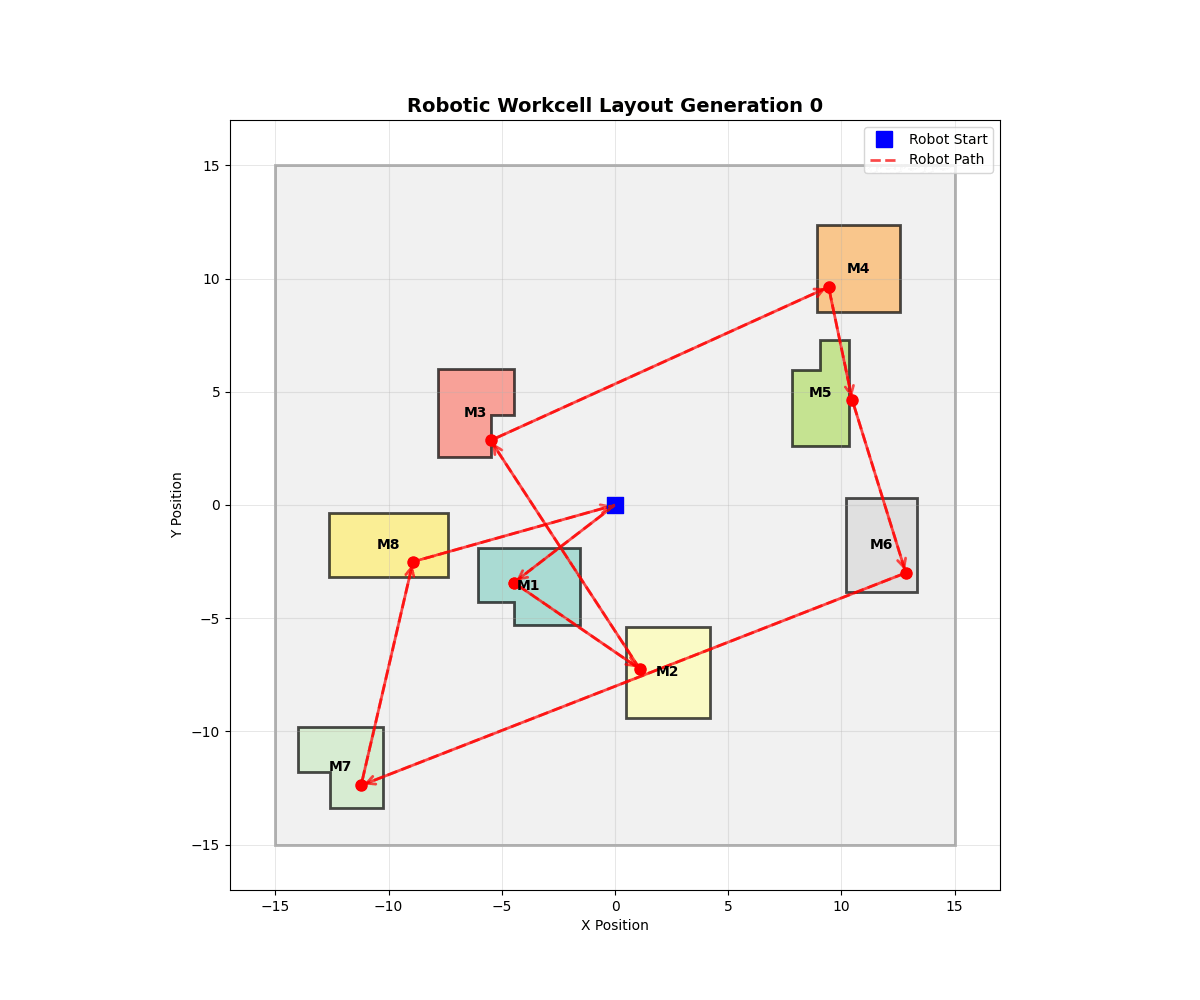
\includegraphics[width=\linewidth]{results_pure_ga_evolution/gen0.png}
        \caption{Generation 0}
    \end{subfigure}
    \hfill
    \begin{subfigure}[b]{0.45\linewidth}
        \centering
        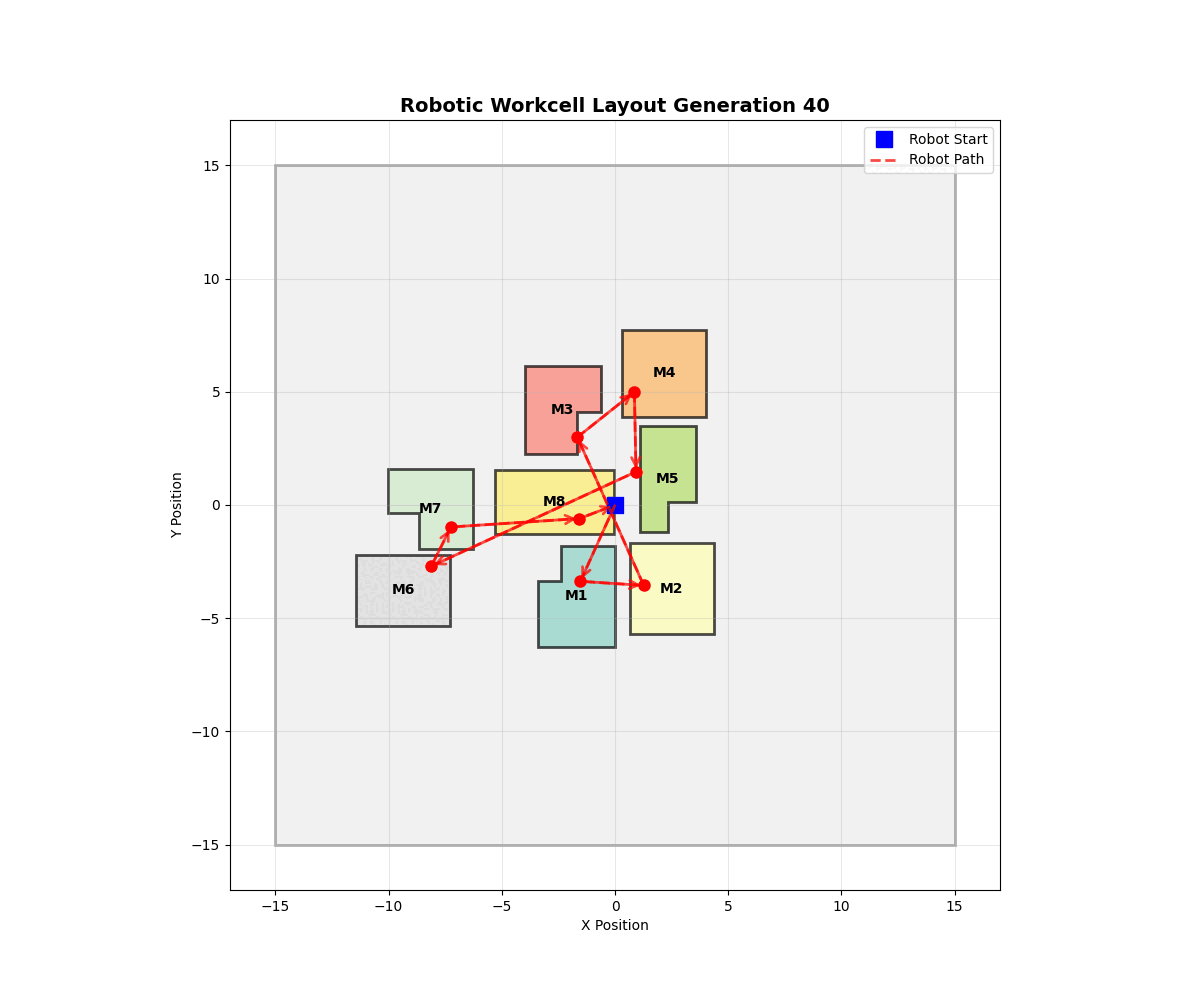
\includegraphics[width=\linewidth]{results_pure_ga_evolution/gen40.png}
        \caption{Generation 40}
    \end{subfigure}

    \vspace{0.5cm}

    \begin{subfigure}[b]{0.45\linewidth}
        \centering
        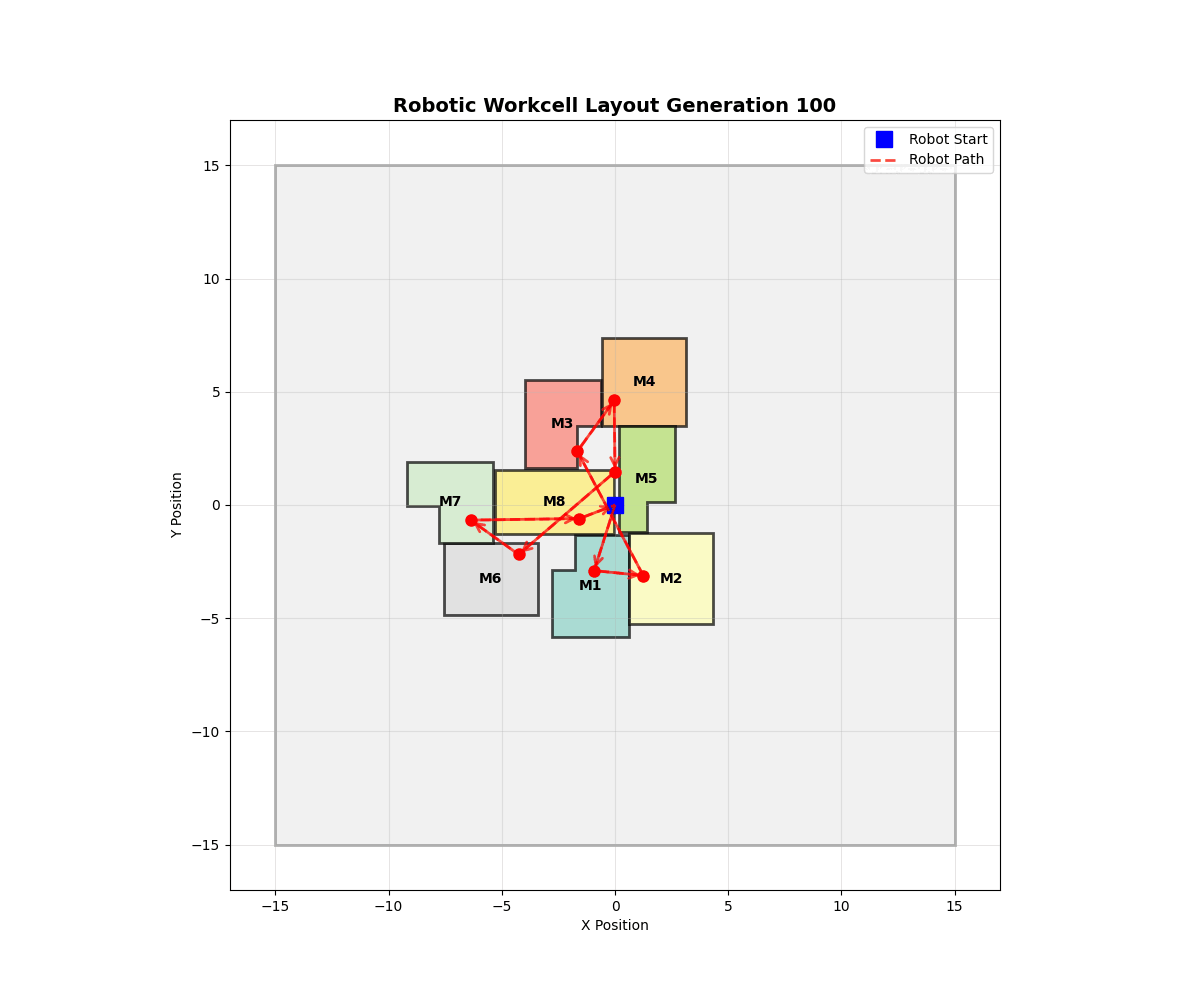
\includegraphics[width=\linewidth]{results_pure_ga_evolution/gen100.png}
        \caption{Generation 100}
    \end{subfigure}
    \hfill
    \begin{subfigure}[b]{0.45\linewidth}
        \centering
        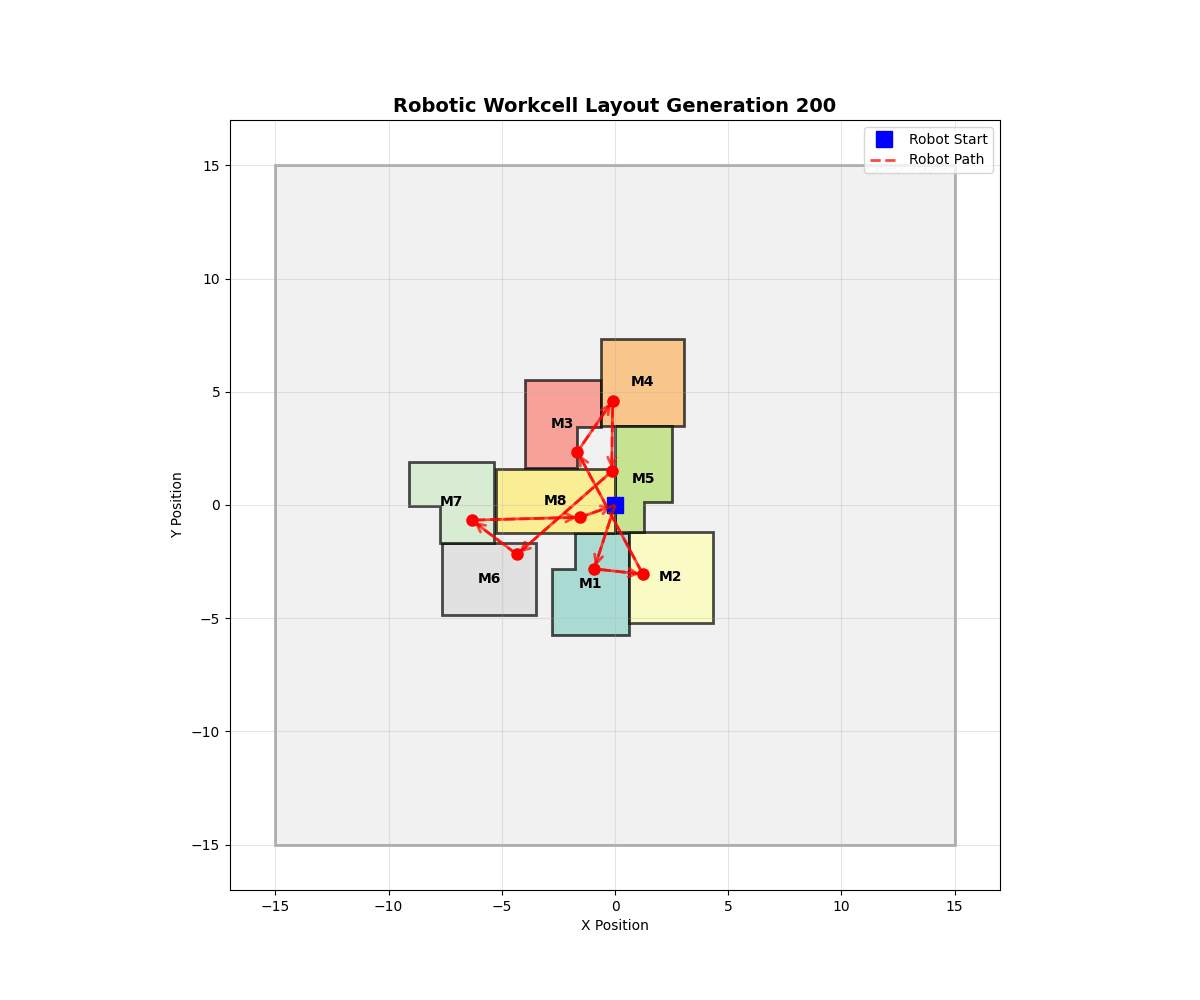
\includegraphics[width=\linewidth]{results_pure_ga_evolution/gen200.png}
        \caption{Generation 200}
    \end{subfigure}

    \caption{Evolution of the robotic workcell layout at selected generations.}
\end{figure}

%----------------------------------------
\subsection{Initial vs Final Comparison}
%----------------------------------------

\begin{figure}[H]
    \centering
    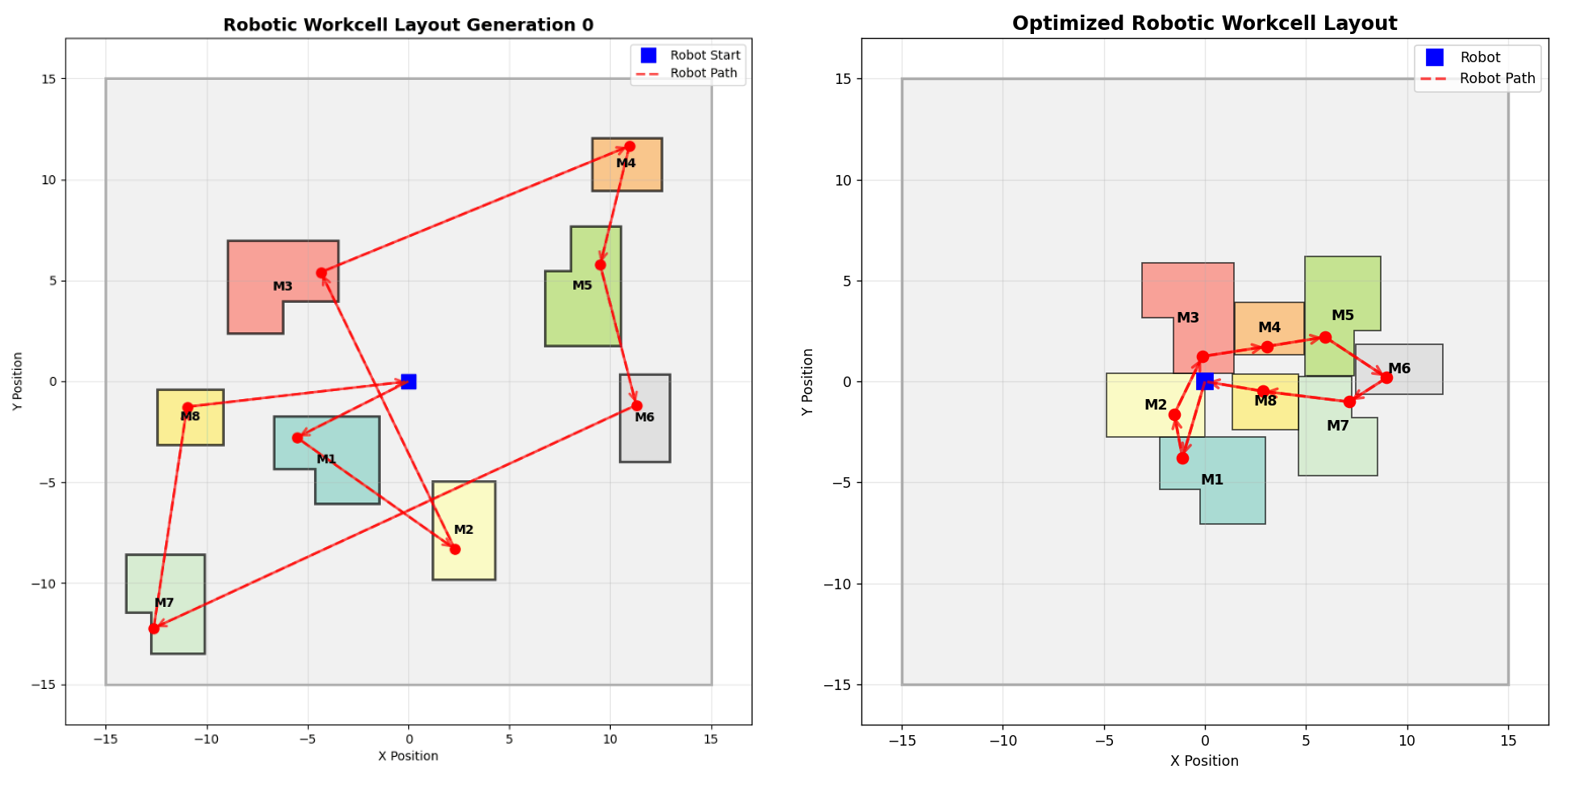
\includegraphics[width=0.8\linewidth]{results_pure_ga_evolution/comparison.png}
    \caption{Comparison between initial and final optimized layouts.}
\end{figure}

\section{Appendix: GA Grid Search Figures}
%====================================================
\subsection{Population Size = 100}
%====================================================

\subsubsection{Generations = 100}
\begin{figure}[H]
    \centering
    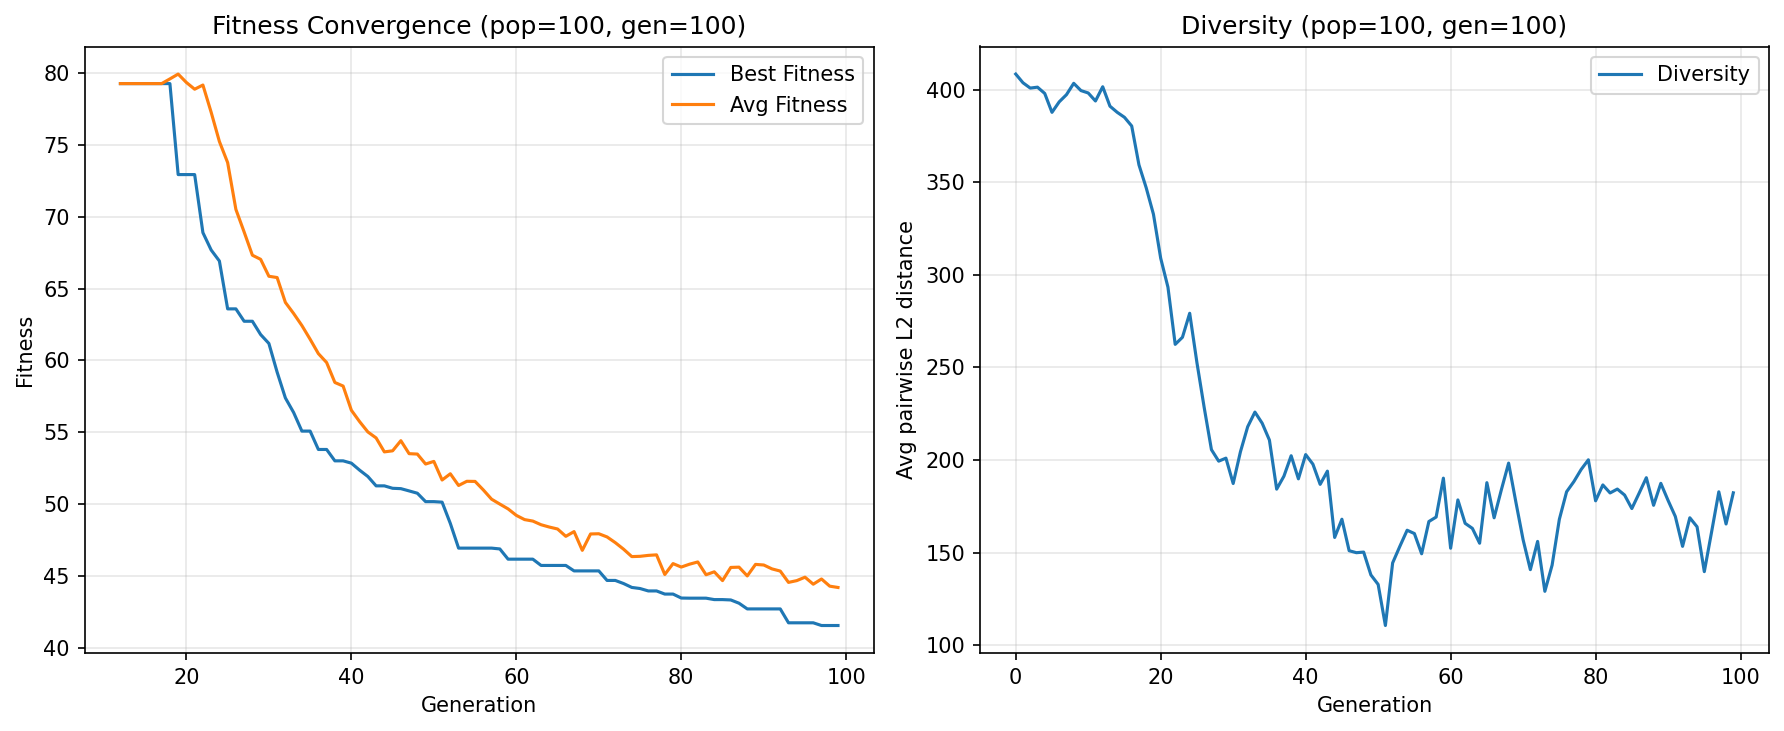
\includegraphics[width=0.9\linewidth]{ga_grid_results_incremental/pop_100/pop_100_gen_100.png}
    \caption{Fitness convergence and diversity plot for population size 100 and 100 generations.}
\end{figure}

\begin{figure}[H]
    \centering
    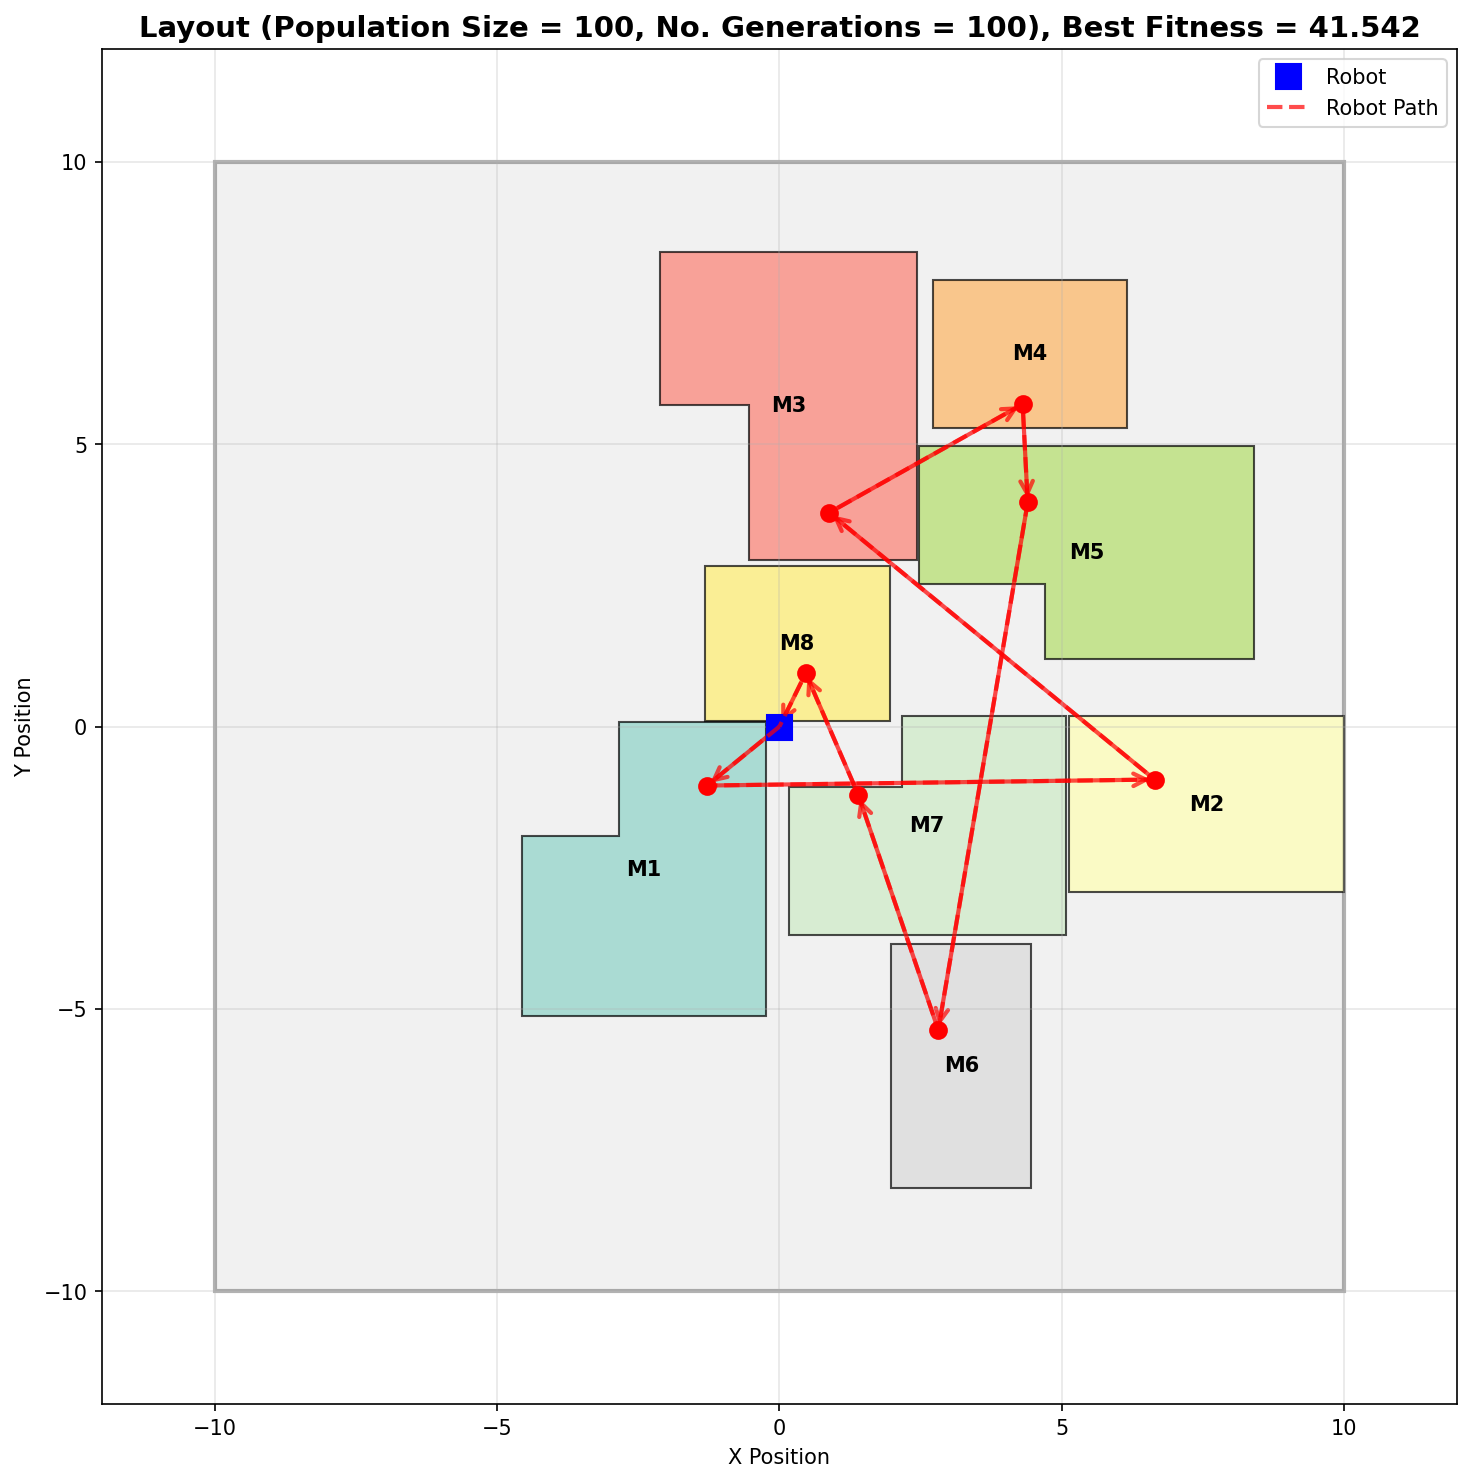
\includegraphics[width=0.7\linewidth]{ga_grid_results_incremental/pop_100/layout_pop_100_gen_100.png}
    \caption{Final optimized layout for population size 100 and 100 generations.}
\end{figure}

\clearpage

\subsubsection{Generations = 200}
\begin{figure}[H]
    \centering
    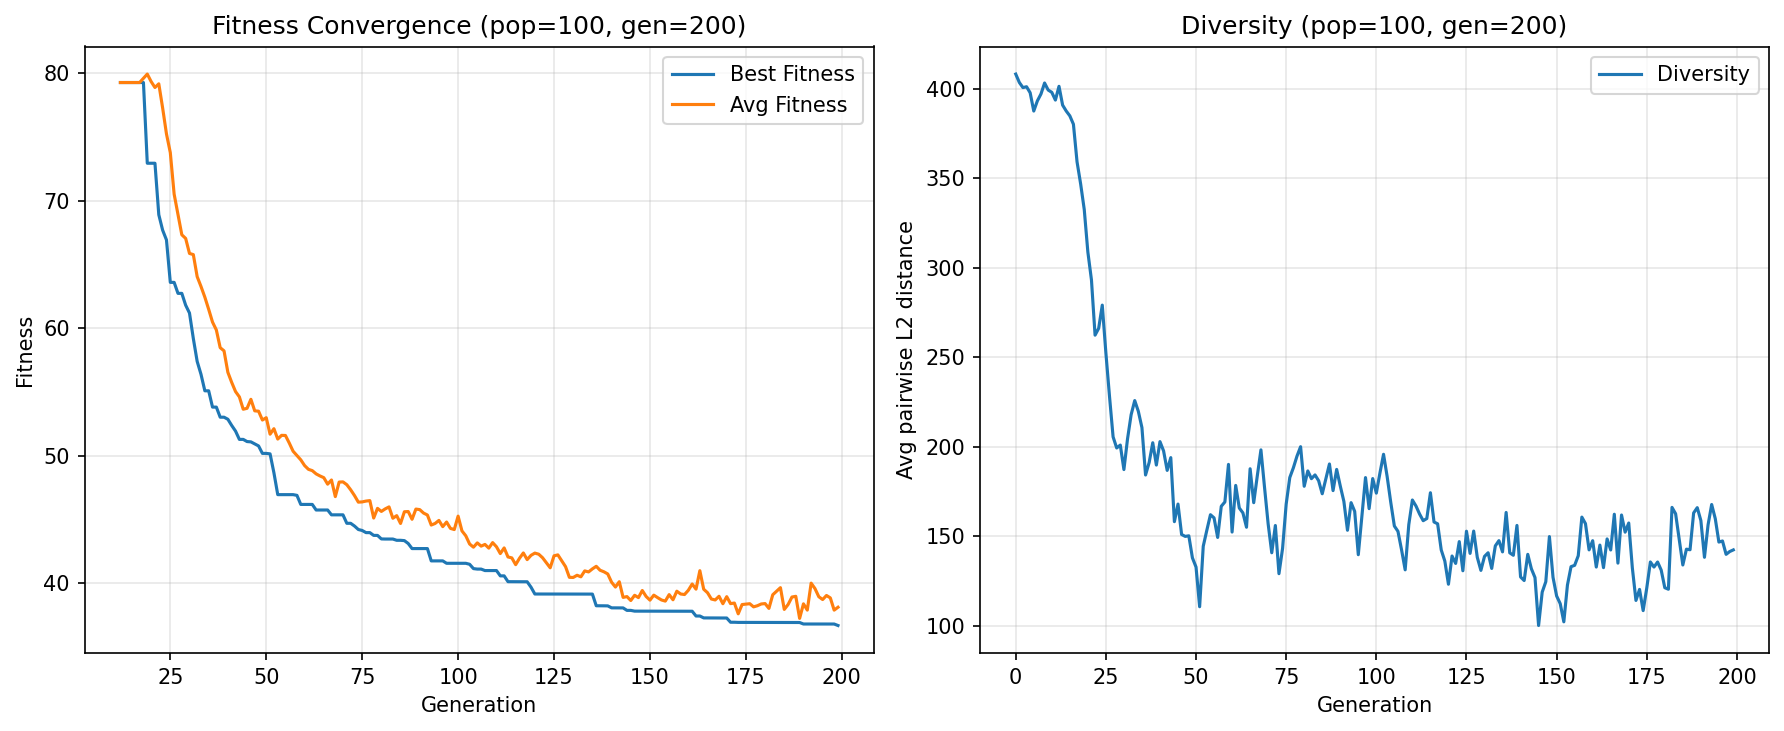
\includegraphics[width=0.9\linewidth]{ga_grid_results_incremental/pop_100/pop_100_gen_200.png}
    \caption{Fitness convergence and diversity plot for population size 100 and 200 generations.}
\end{figure}

\begin{figure}[H]
    \centering
    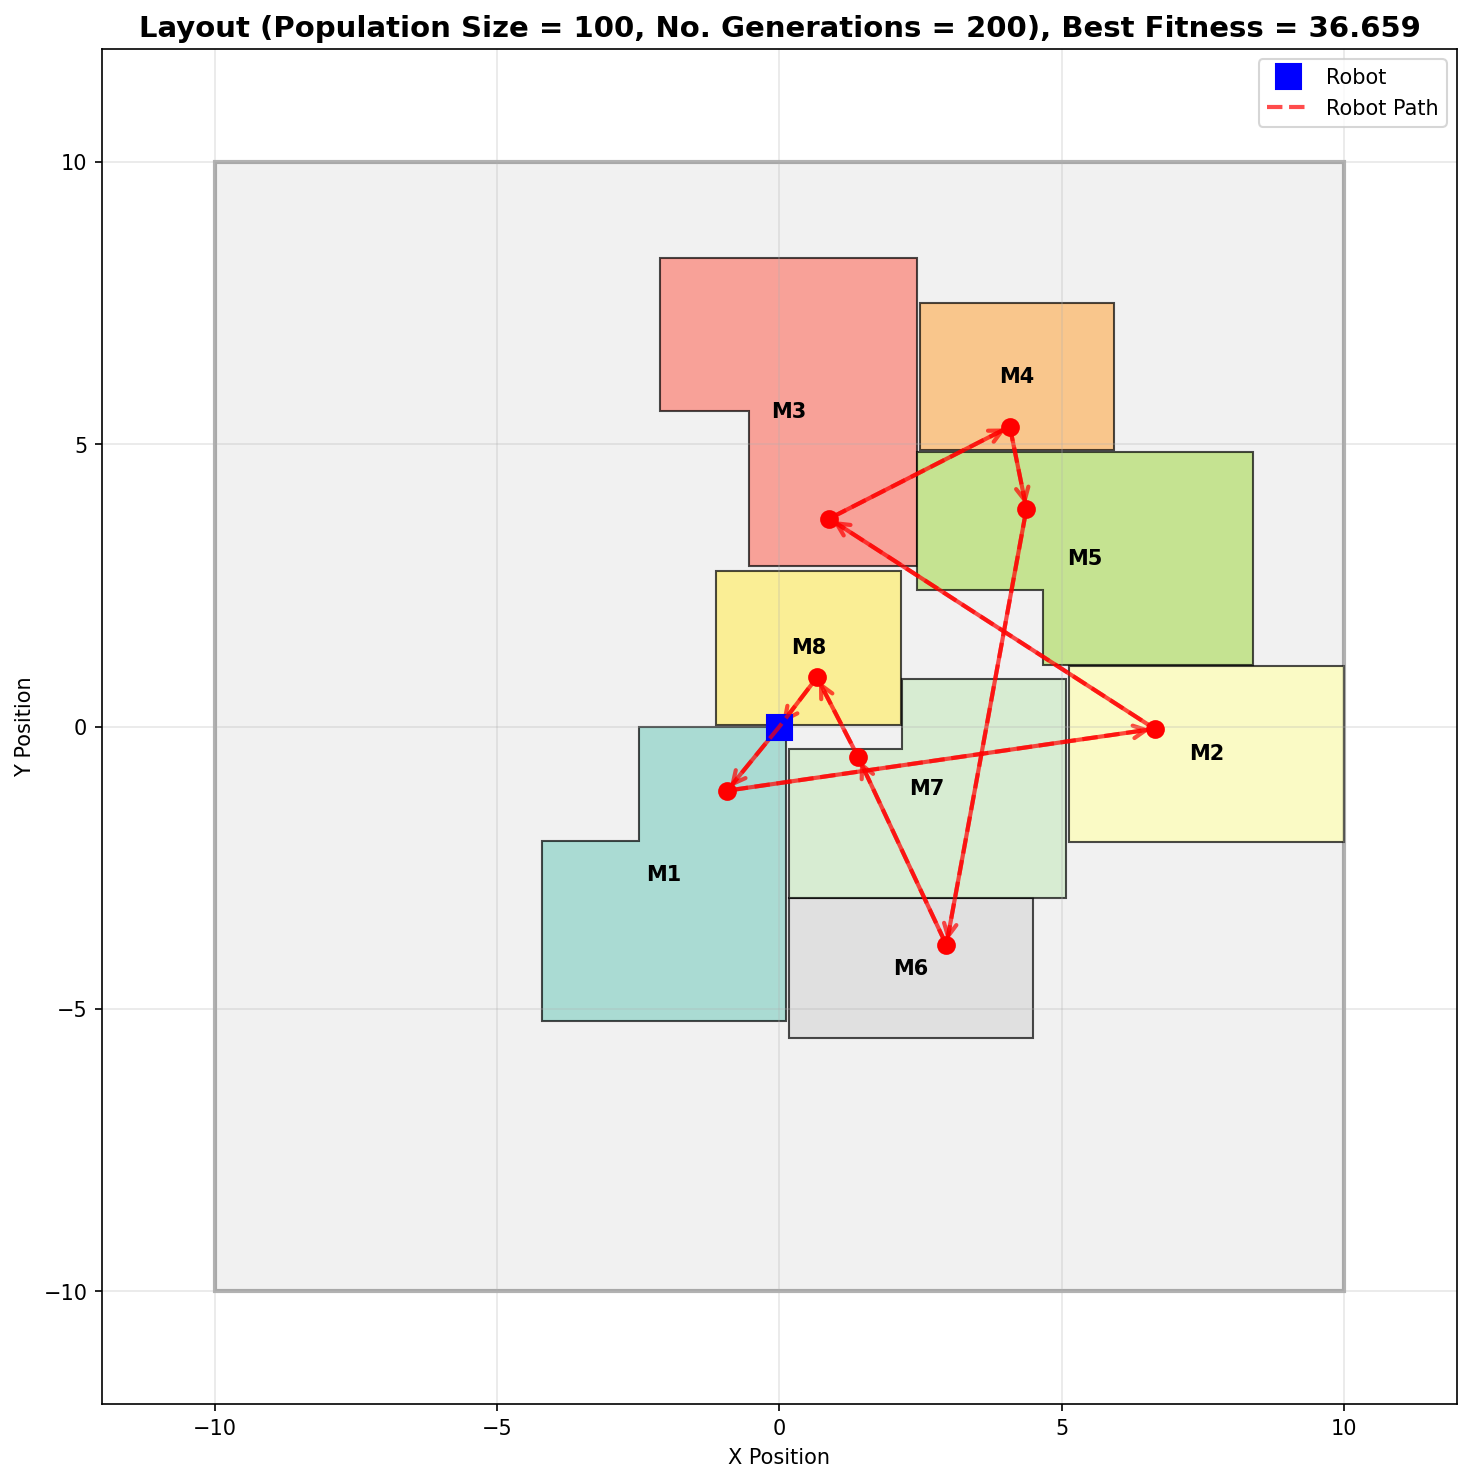
\includegraphics[width=0.7\linewidth]{ga_grid_results_incremental/pop_100/layout_pop_100_gen_200.png}
    \caption{Final optimized layout for population size 100 and 200 generations.}
\end{figure}

\clearpage

\subsubsection{Generations = 500}
\begin{figure}[H]
    \centering
    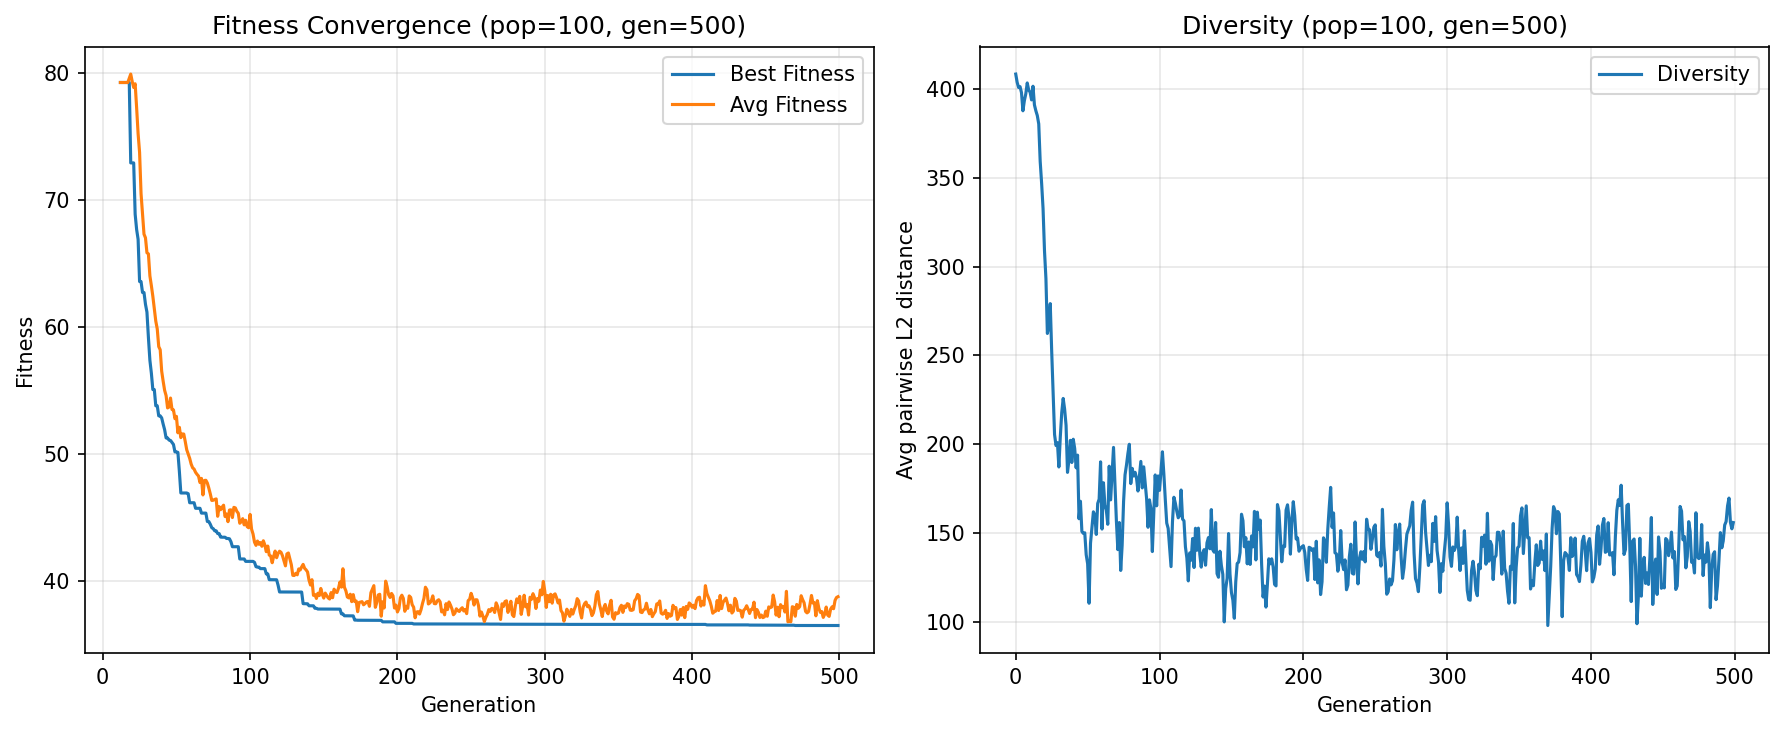
\includegraphics[width=0.9\linewidth]{ga_grid_results_incremental/pop_100/pop_100_gen_500.png}
    \caption{Fitness convergence and diversity plot for population size 100 and 500 generations.}
\end{figure}

\begin{figure}[H]
    \centering
    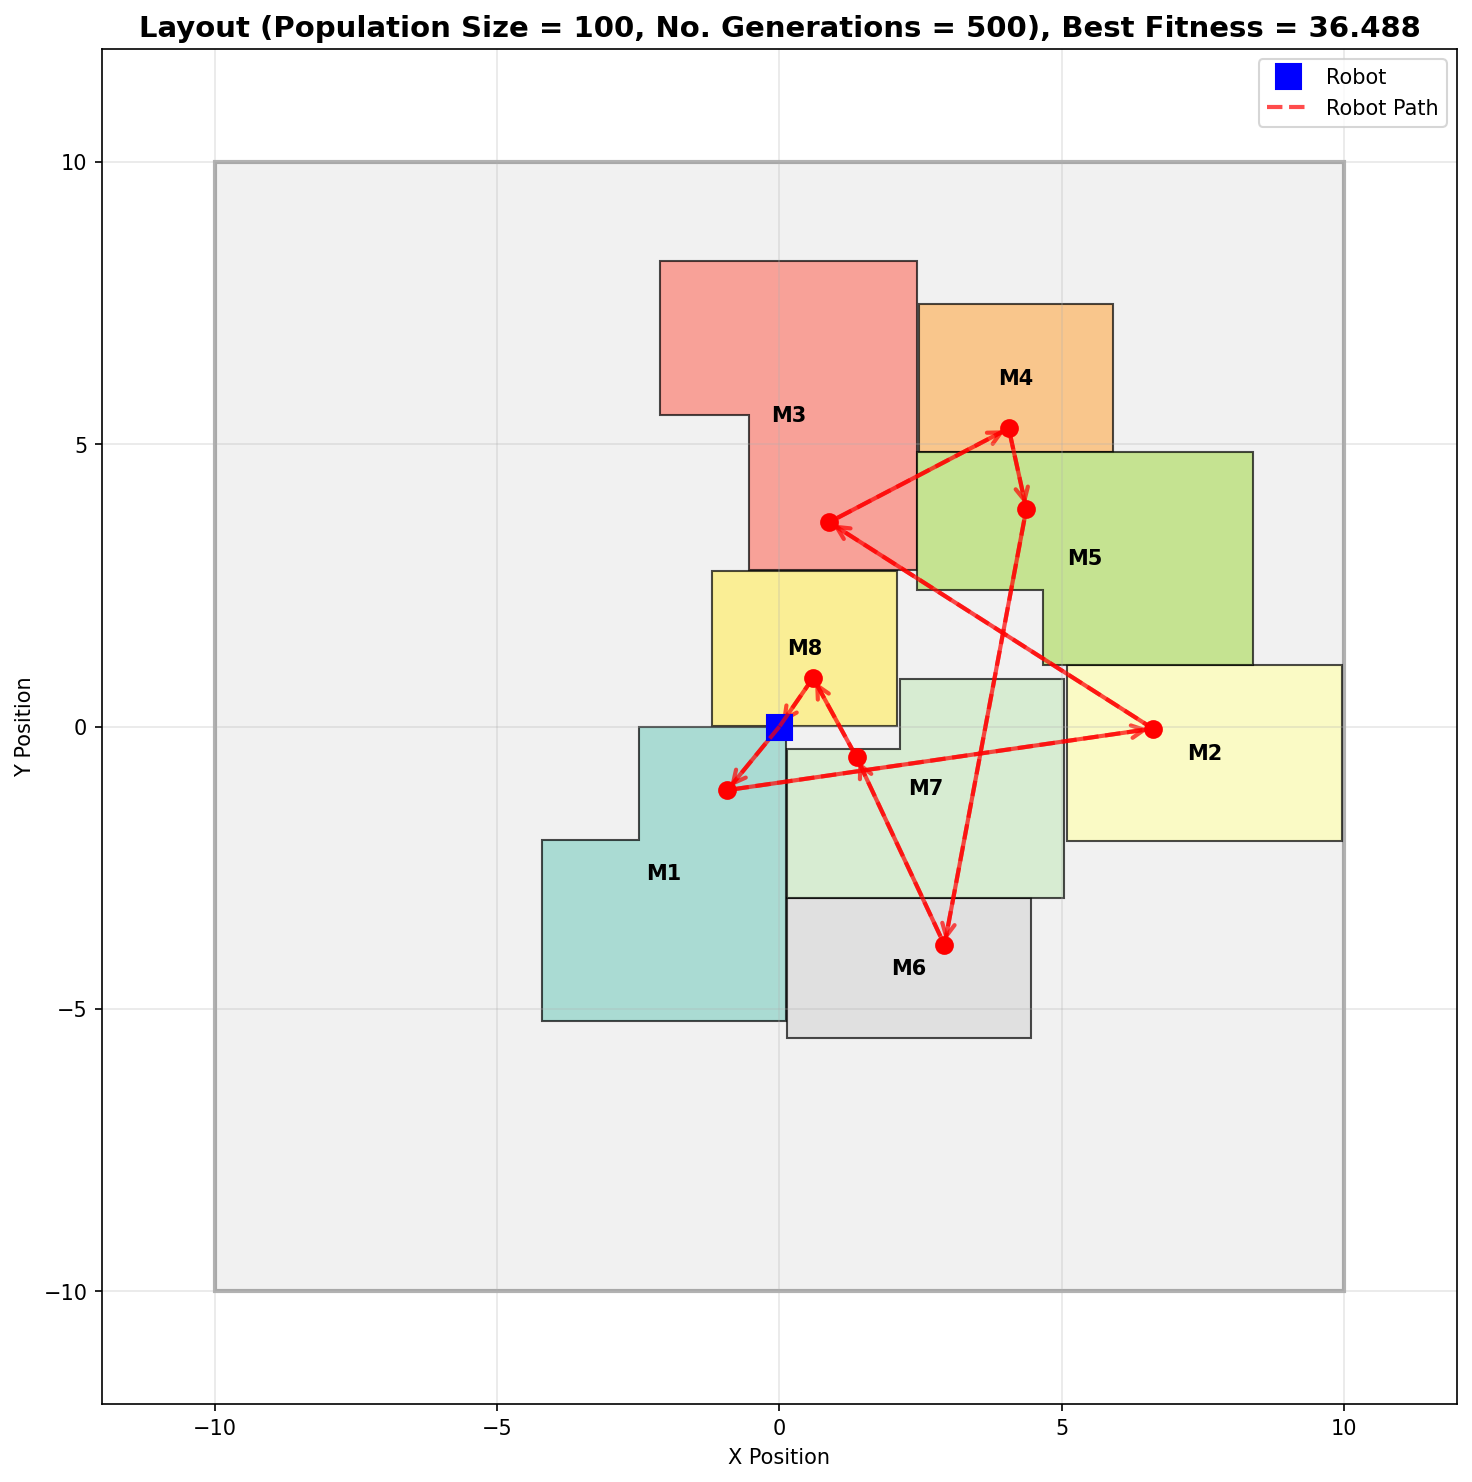
\includegraphics[width=0.7\linewidth]{ga_grid_results_incremental/pop_100/layout_pop_100_gen_500.png}
    \caption{Final optimized layout for population size 100 and 500 generations.}
\end{figure}

\clearpage

\subsubsection{Generations = 1000}
\begin{figure}[H]
    \centering
    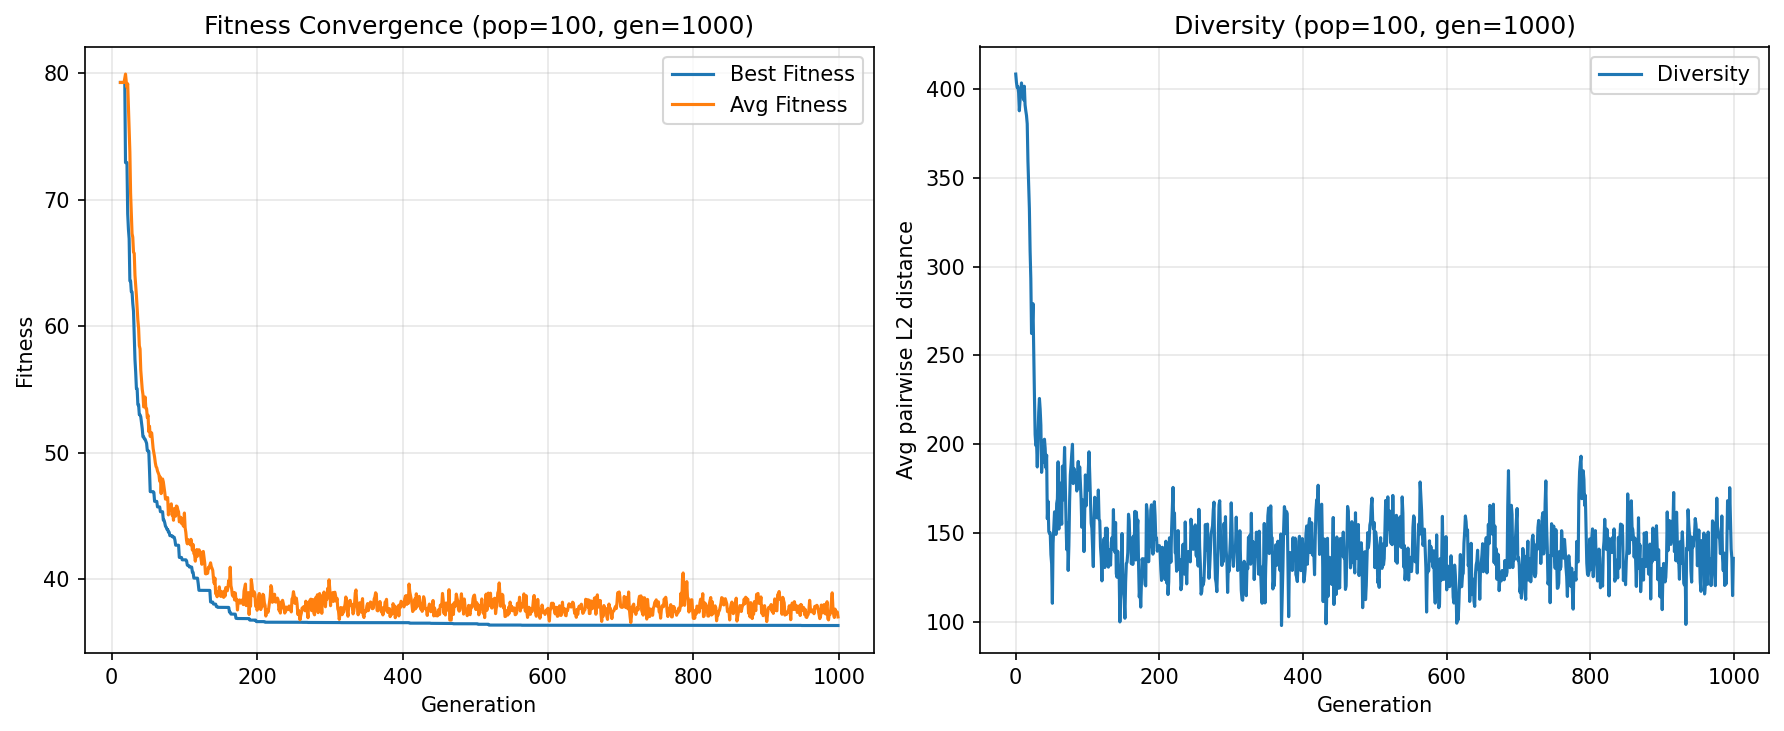
\includegraphics[width=0.9\linewidth]{ga_grid_results_incremental/pop_100/pop_100_gen_1000.png}
    \caption{Fitness convergence and diversity plot for population size 100 and 1000 generations.}
\end{figure}

\begin{figure}[H]
    \centering
    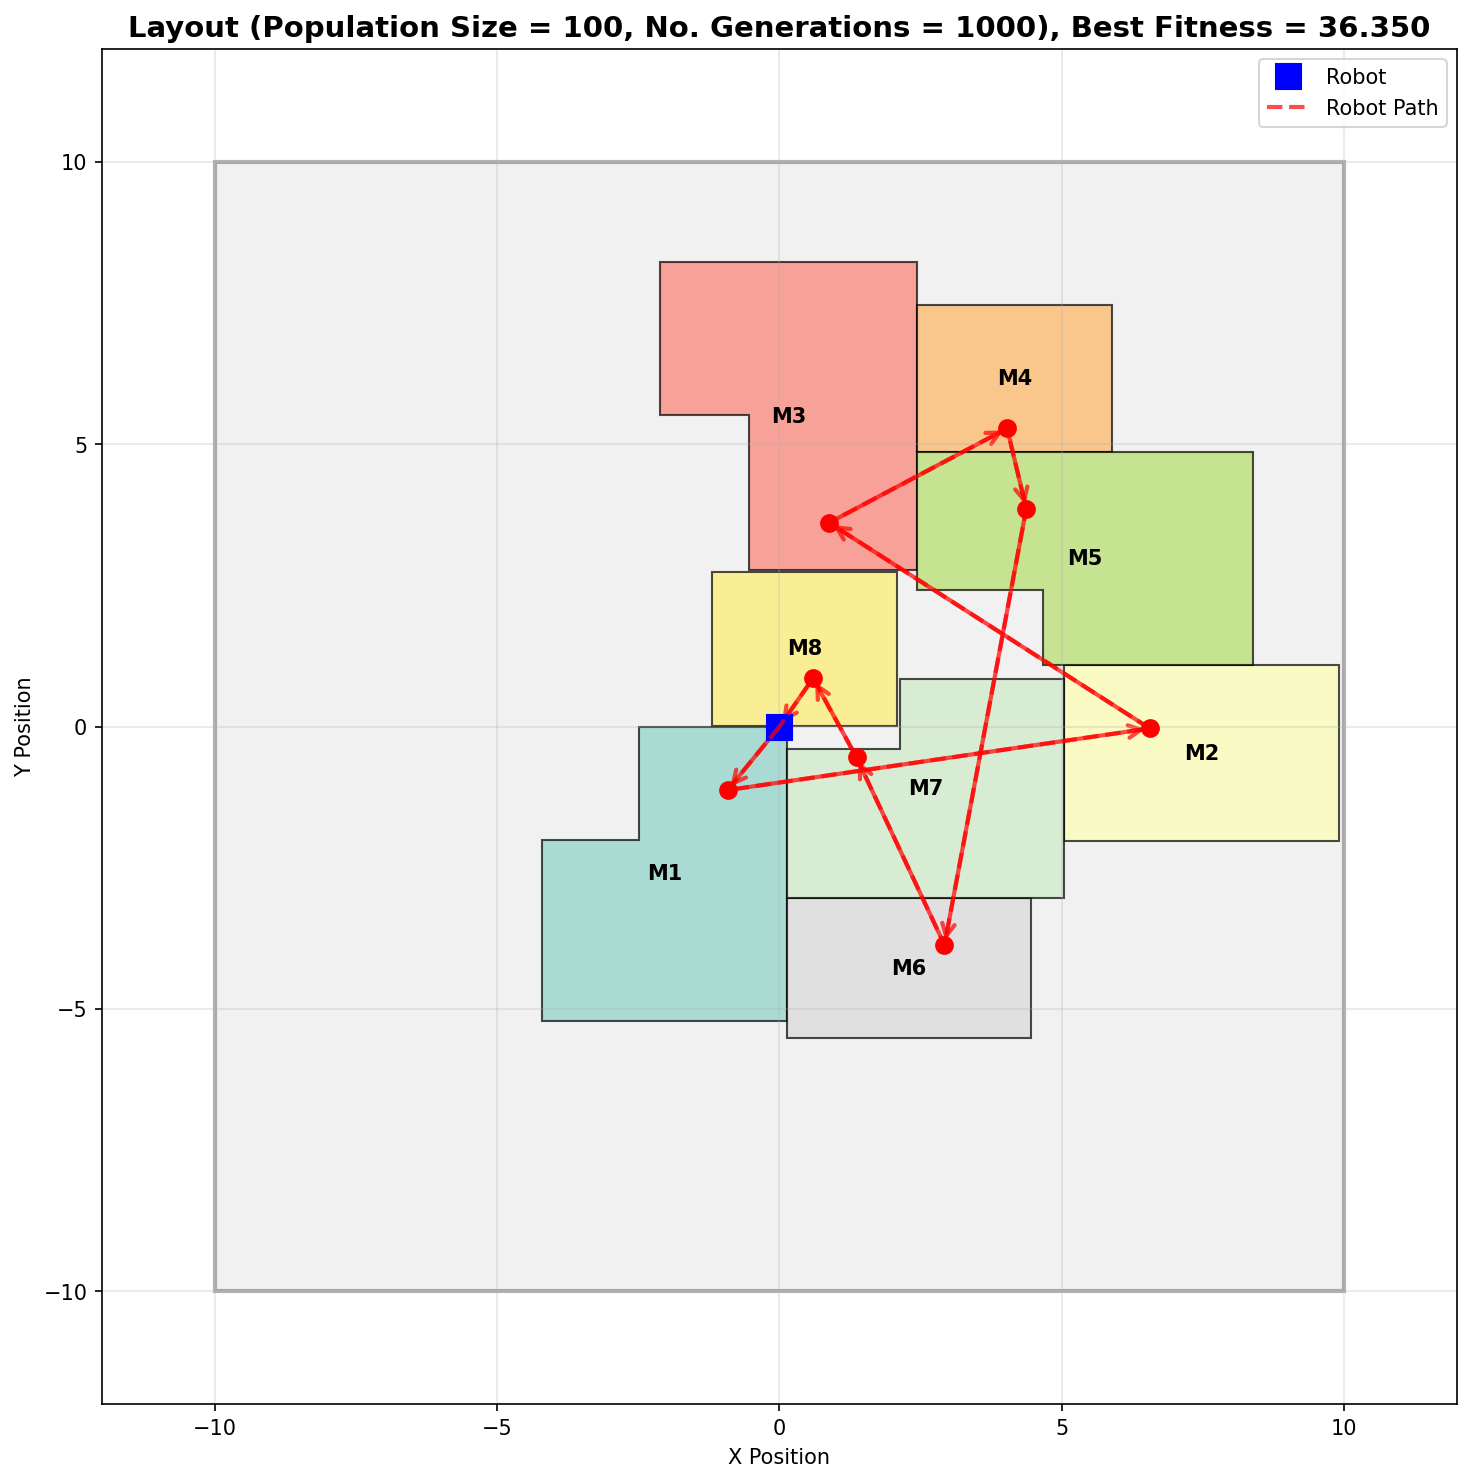
\includegraphics[width=0.7\linewidth]{ga_grid_results_incremental/pop_100/layout_pop_100_gen_1000.png}
    \caption{Final optimized layout for population size 100 and 1000 generations.}
\end{figure}

\clearpage

\subsubsection{Generations = 2000}
\begin{figure}[H]
    \centering
    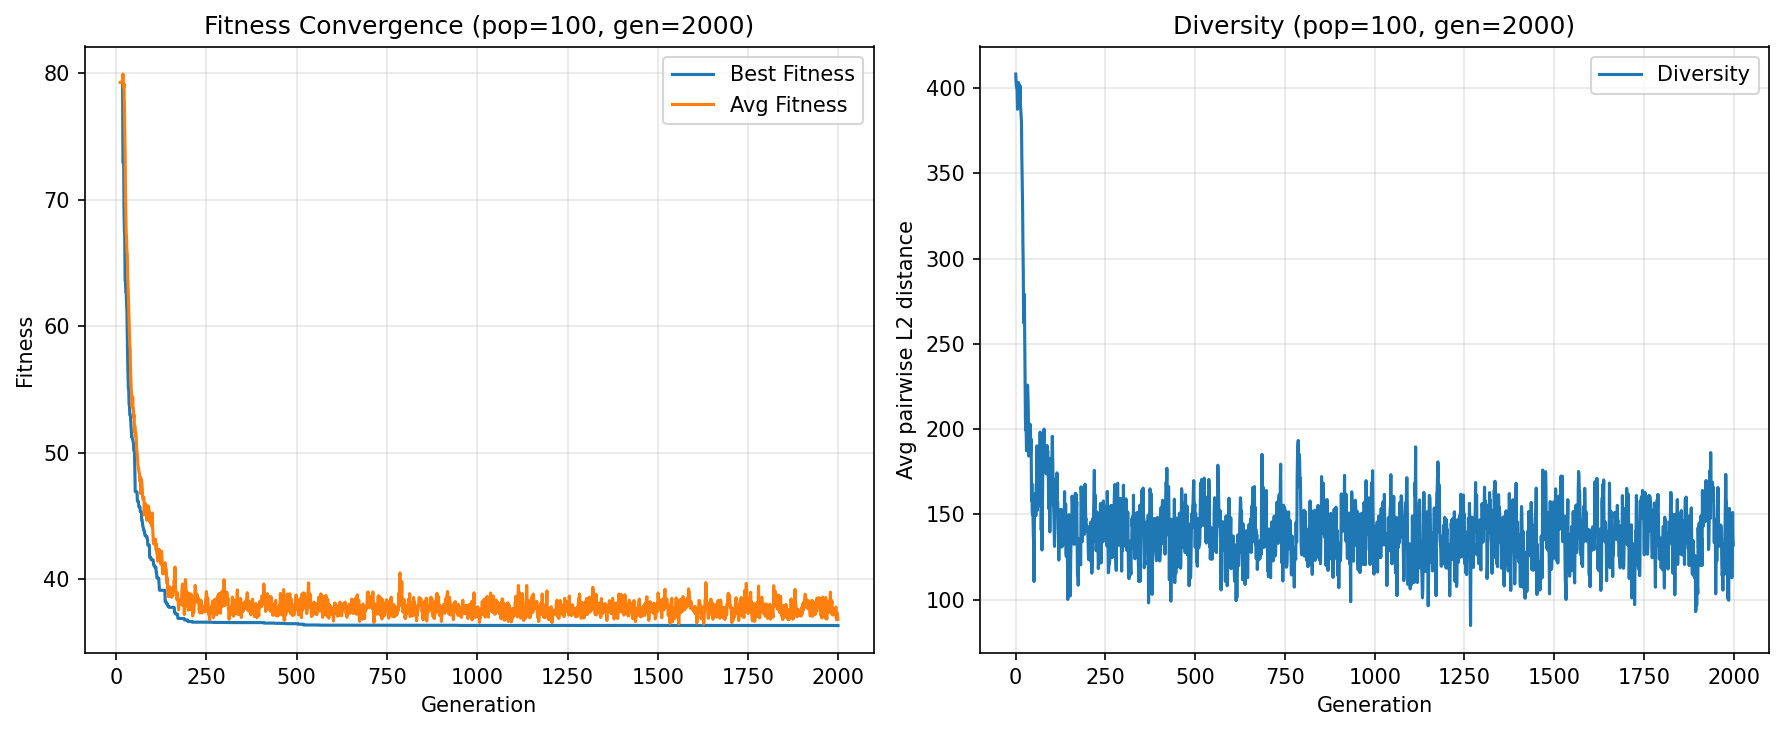
\includegraphics[width=0.9\linewidth]{ga_grid_results_incremental/pop_100/pop_100_gen_2000.png}
    \caption{Fitness convergence and diversity plot for population size 100 and 2000 generations.}
\end{figure}

\begin{figure}[H]
    \centering
    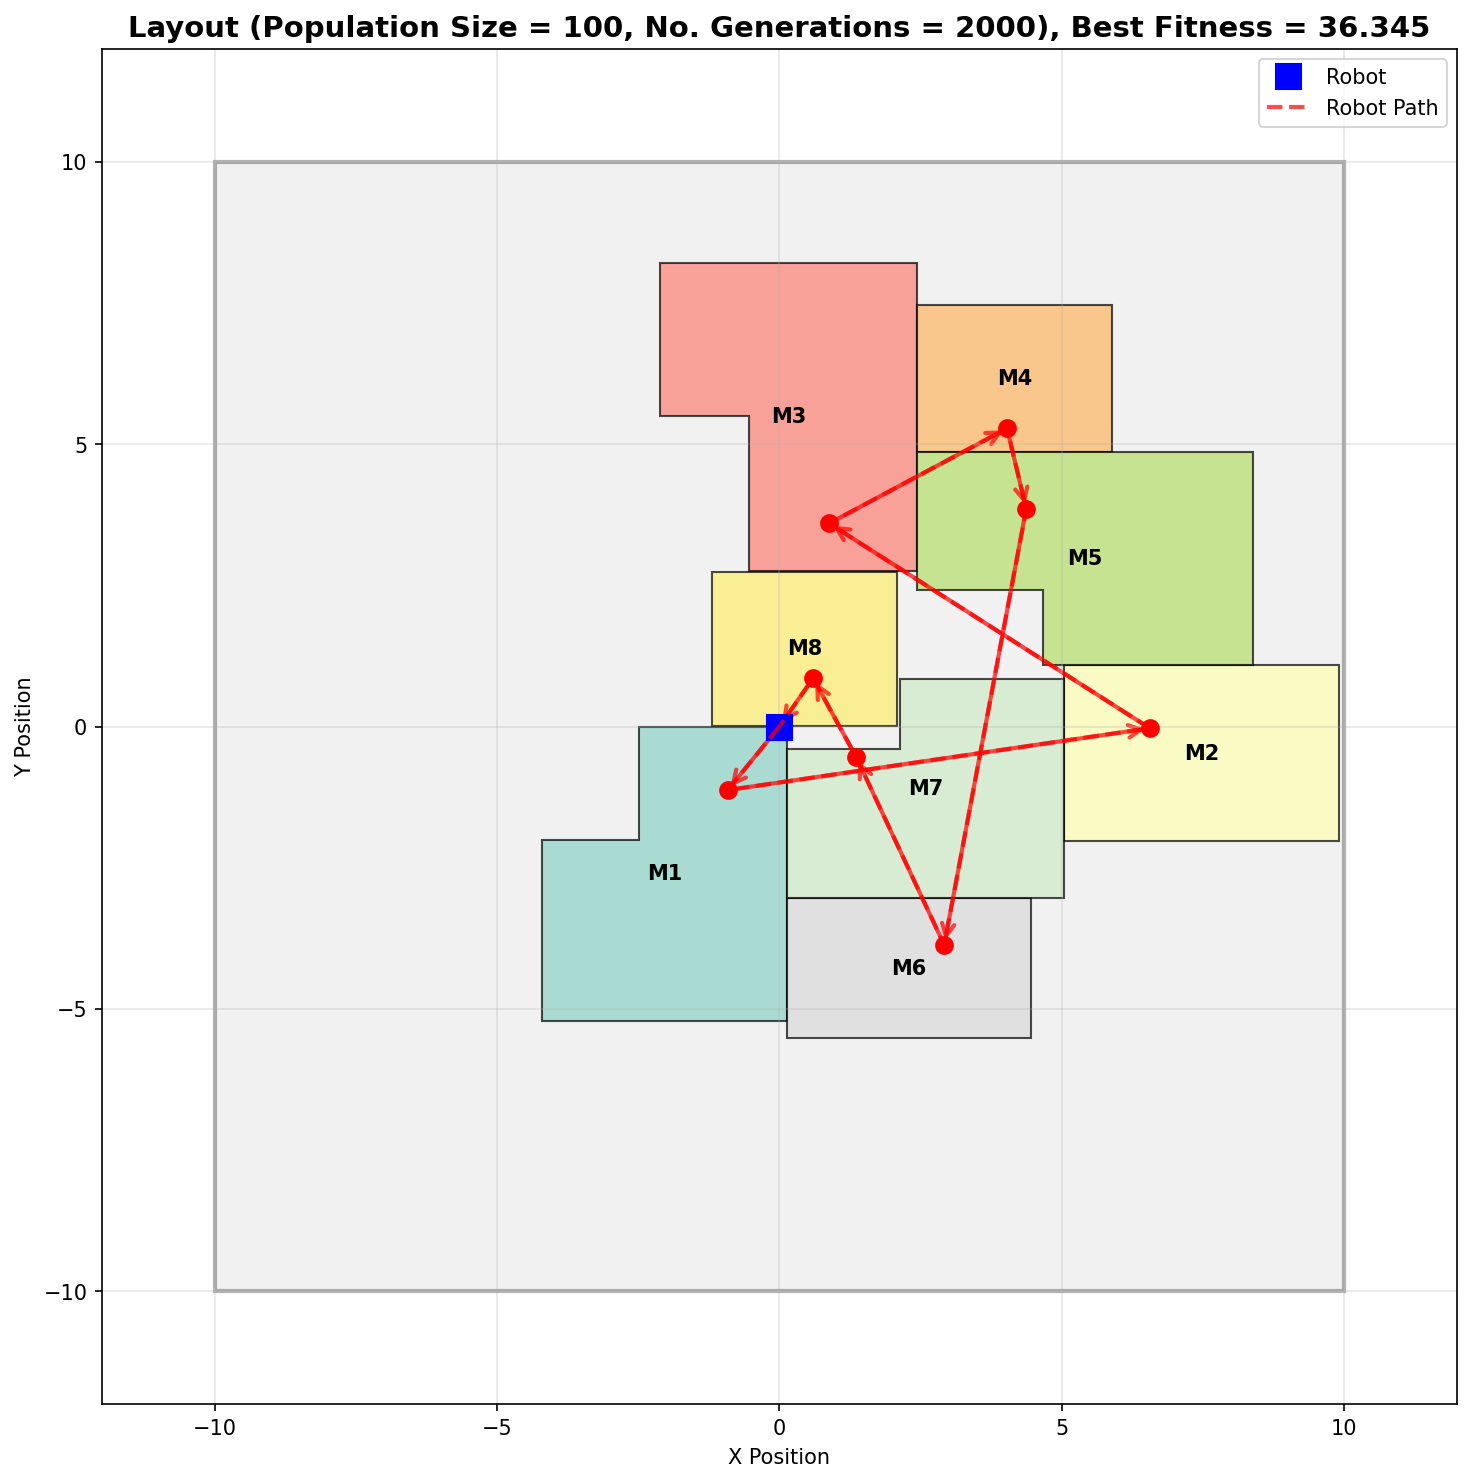
\includegraphics[width=0.7\linewidth]{ga_grid_results_incremental/pop_100/layout_pop_100_gen_2000.png}
    \caption{Final optimized layout for population size 100 and 2000 generations.}
\end{figure}

\clearpage

%====================================================
\subsection{Population Size = 200}
%====================================================

\subsubsection{Generations = 100}
\begin{figure}[H]
    \centering
    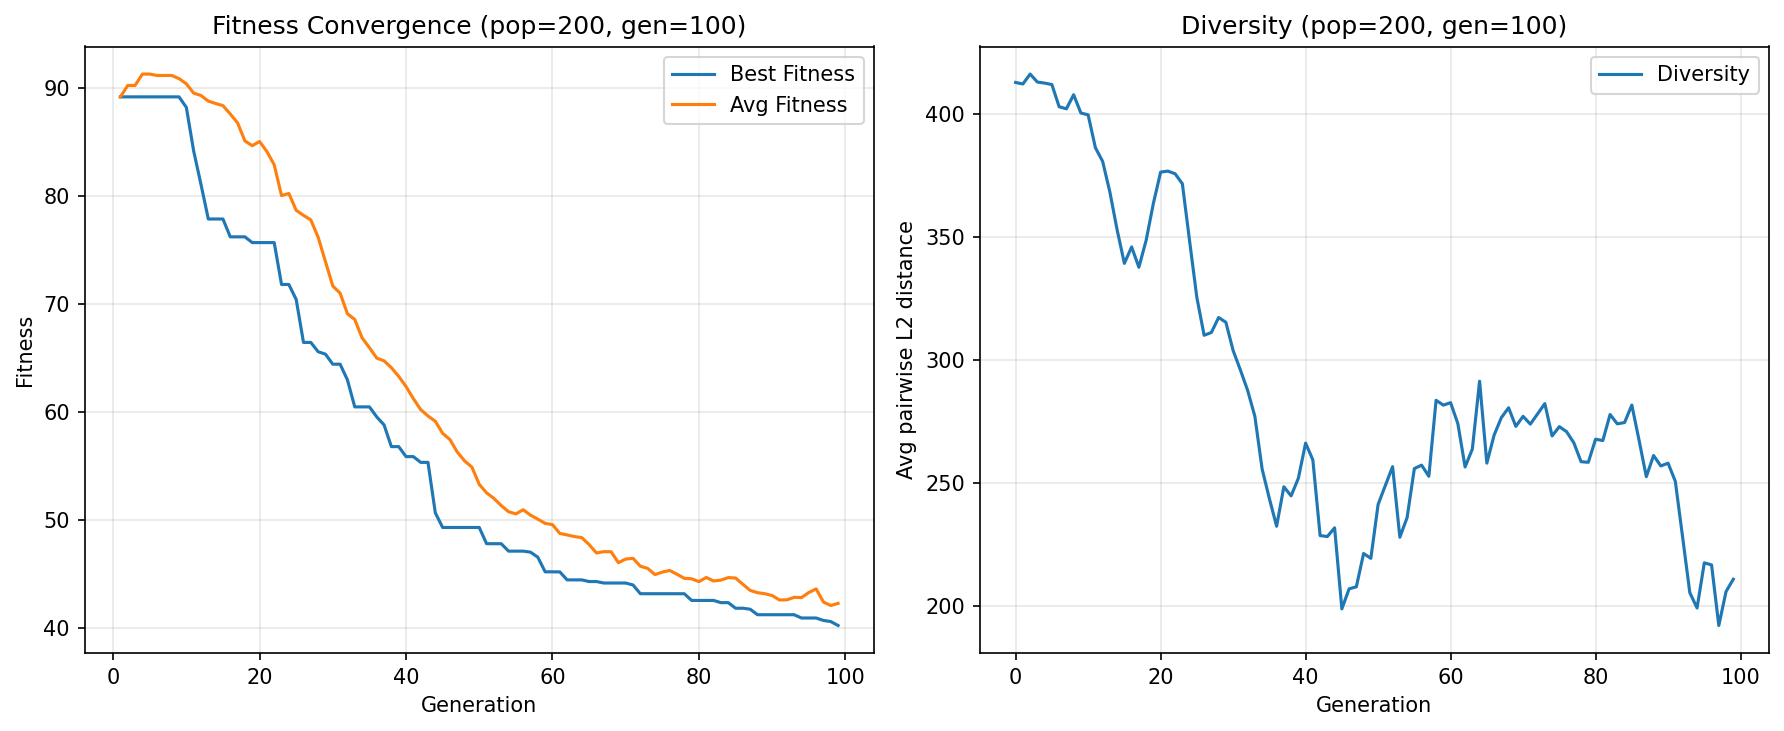
\includegraphics[width=0.9\linewidth]{ga_grid_results_incremental/pop_200/pop_200_gen_100.png}
    \caption{Fitness convergence and diversity plot for population size 200 and 100 generations.}
\end{figure}

\begin{figure}[H]
    \centering
    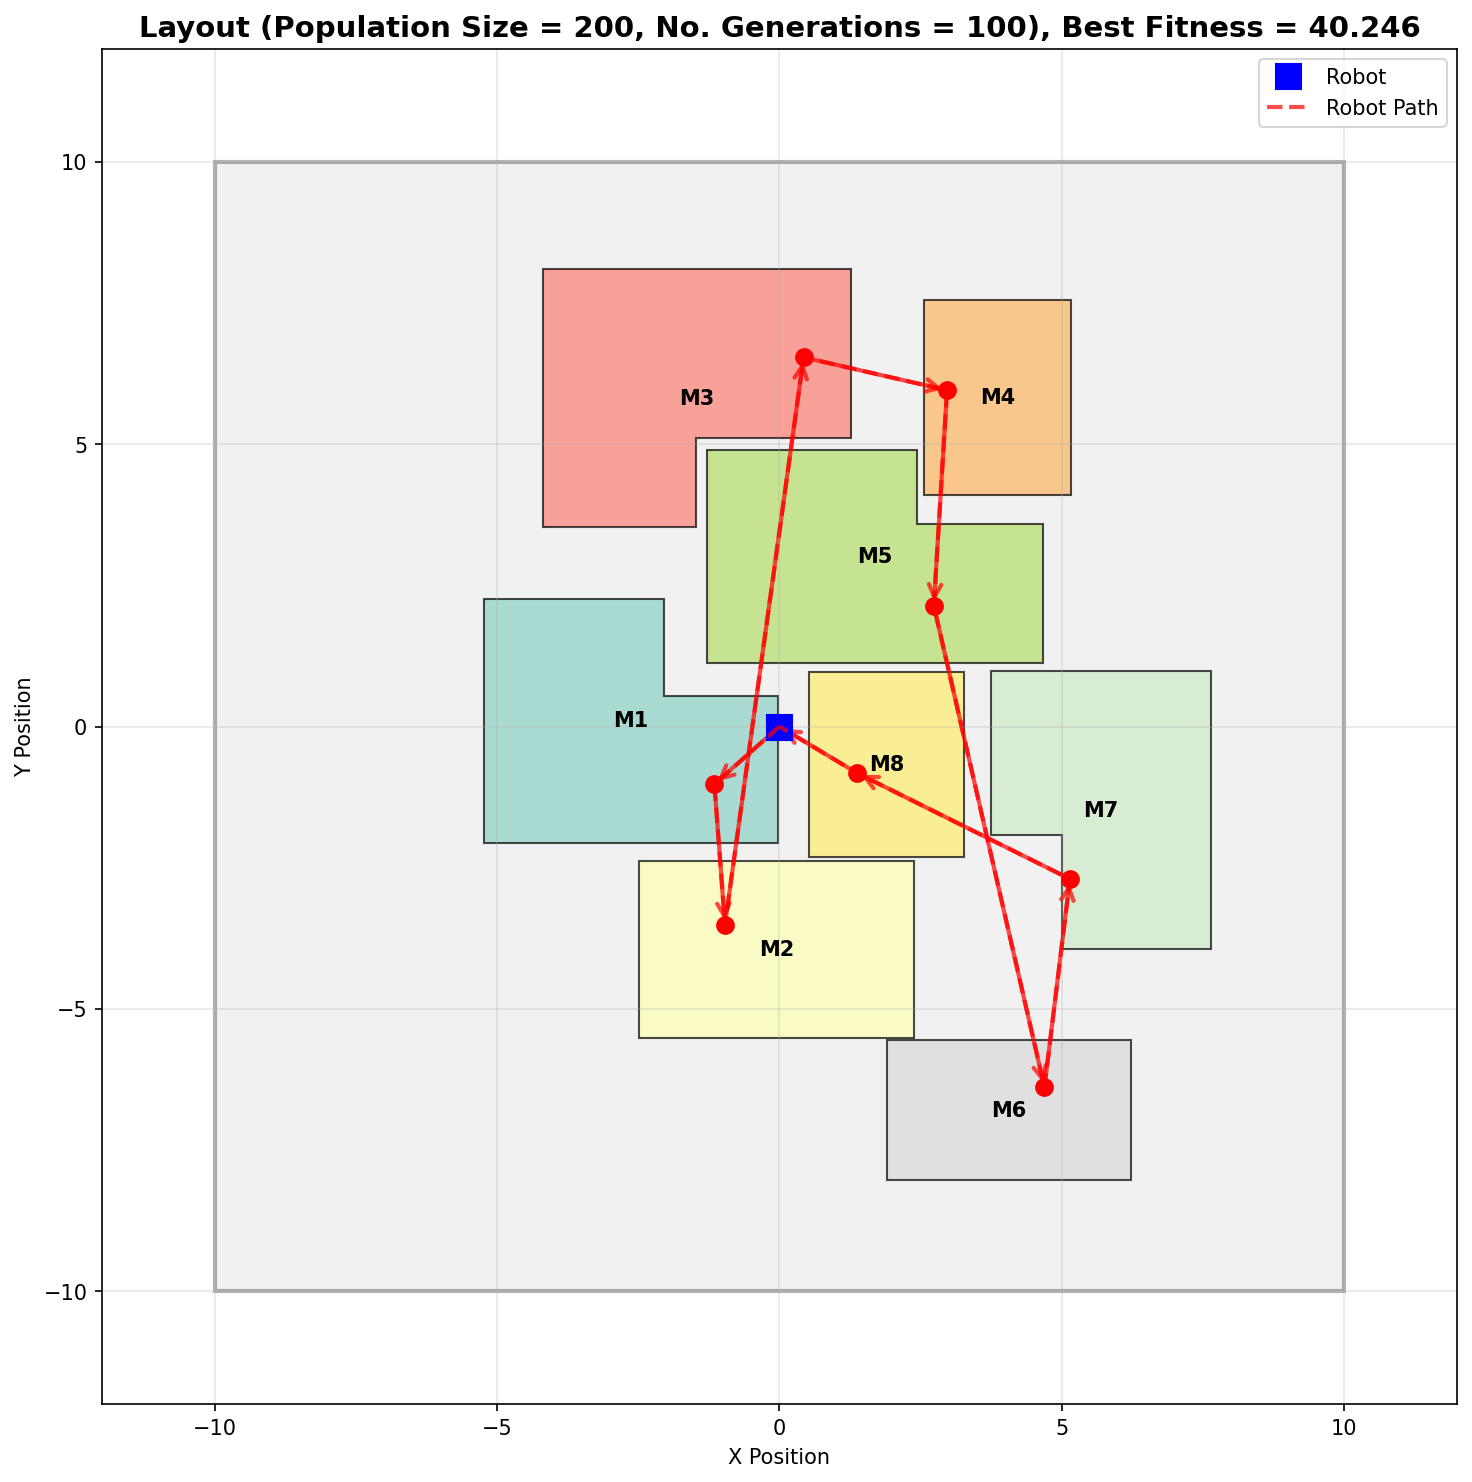
\includegraphics[width=0.7\linewidth]{ga_grid_results_incremental/pop_200/layout_pop_200_gen_100.png}
    \caption{Final optimized layout for population size 200 and 100 generations.}
\end{figure}

\clearpage

\subsubsection{Generations = 200}
\begin{figure}[H]
    \centering
    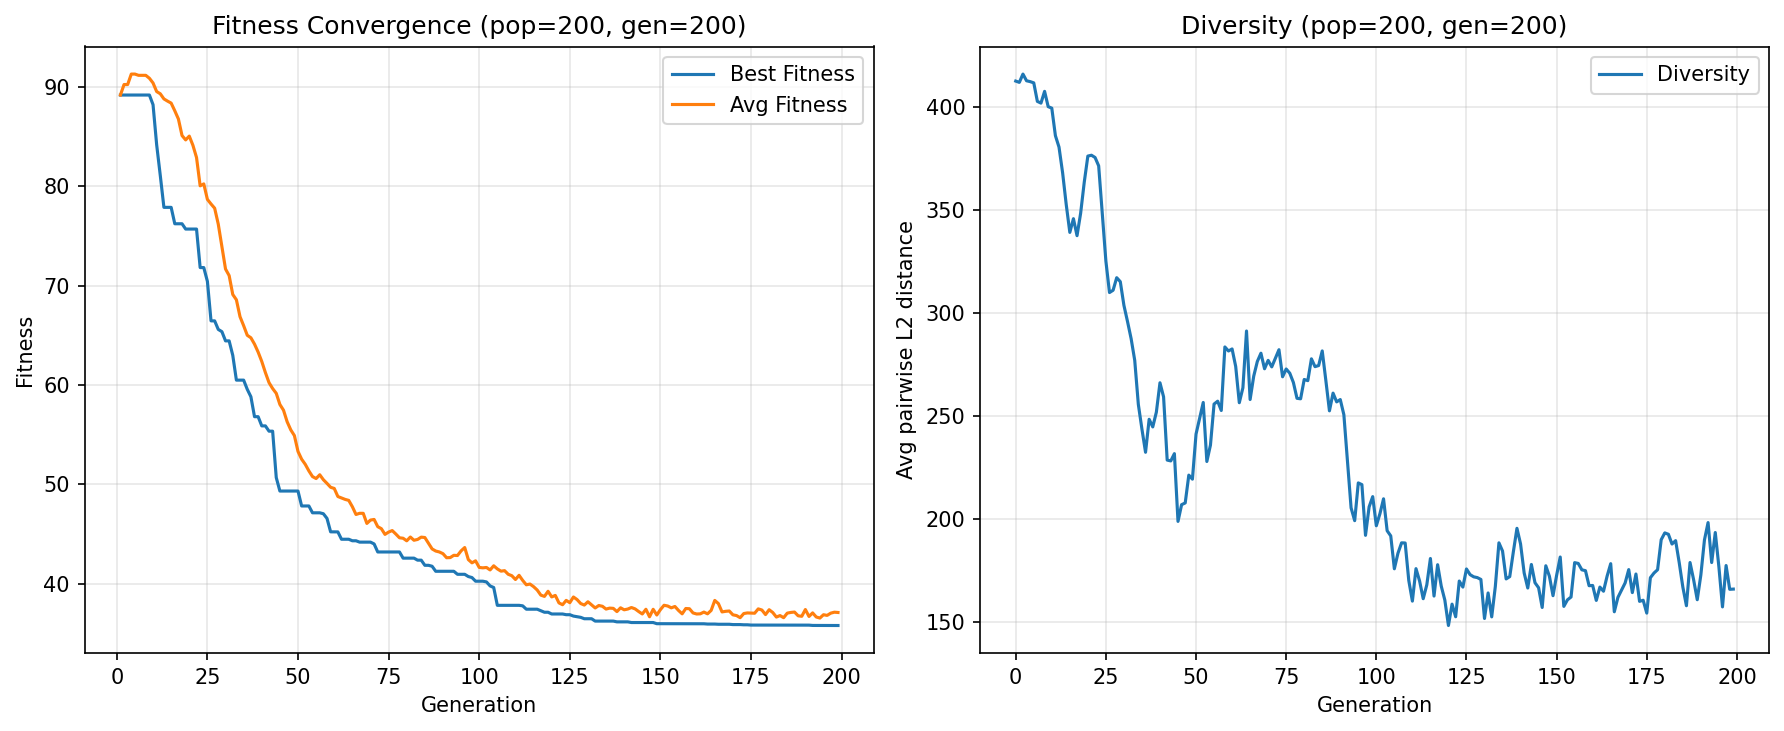
\includegraphics[width=0.9\linewidth]{ga_grid_results_incremental/pop_200/pop_200_gen_200.png}
    \caption{Fitness convergence and diversity plot for population size 200 and 200 generations.}
\end{figure}

\begin{figure}[H]
    \centering
    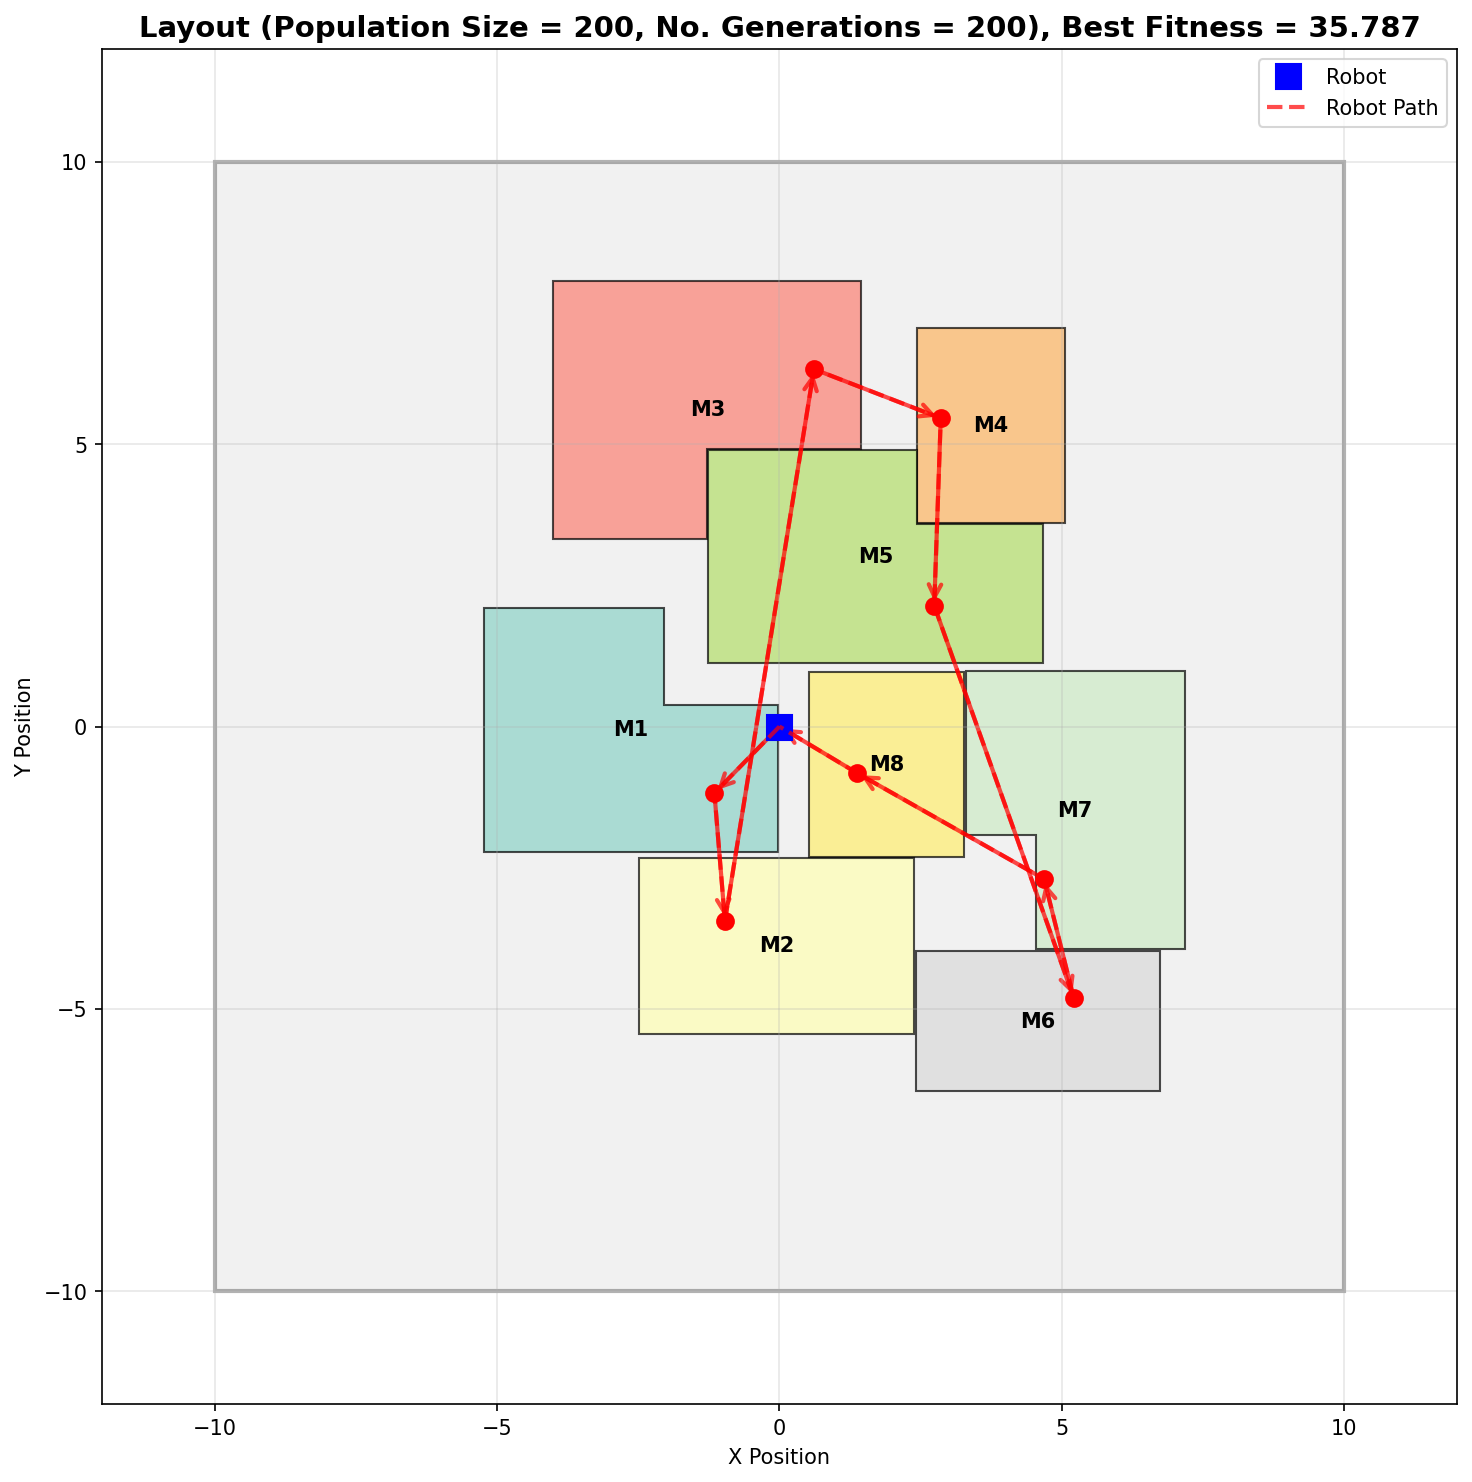
\includegraphics[width=0.7\linewidth]{ga_grid_results_incremental/pop_200/layout_pop_200_gen_200.png}
    \caption{Final optimized layout for population size 200 and 200 generations.}
\end{figure}

\clearpage

\subsubsection{Generations = 500}
\begin{figure}[H]
    \centering
    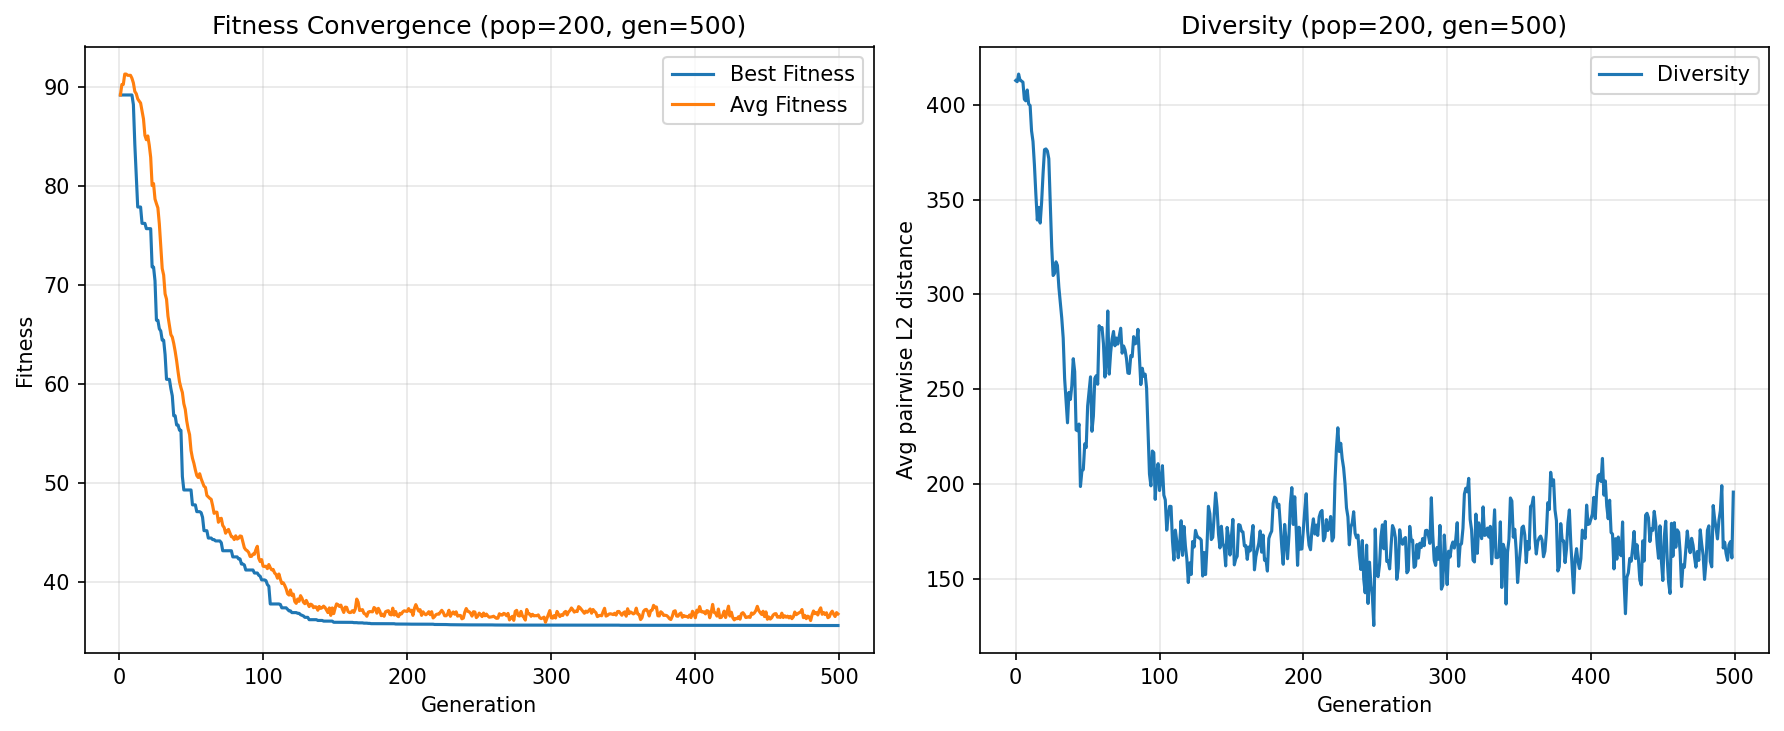
\includegraphics[width=0.9\linewidth]{ga_grid_results_incremental/pop_200/pop_200_gen_500.png}
    \caption{Fitness convergence and diversity plot for population size 200 and 500 generations.}
\end{figure}

\begin{figure}[H]
    \centering
    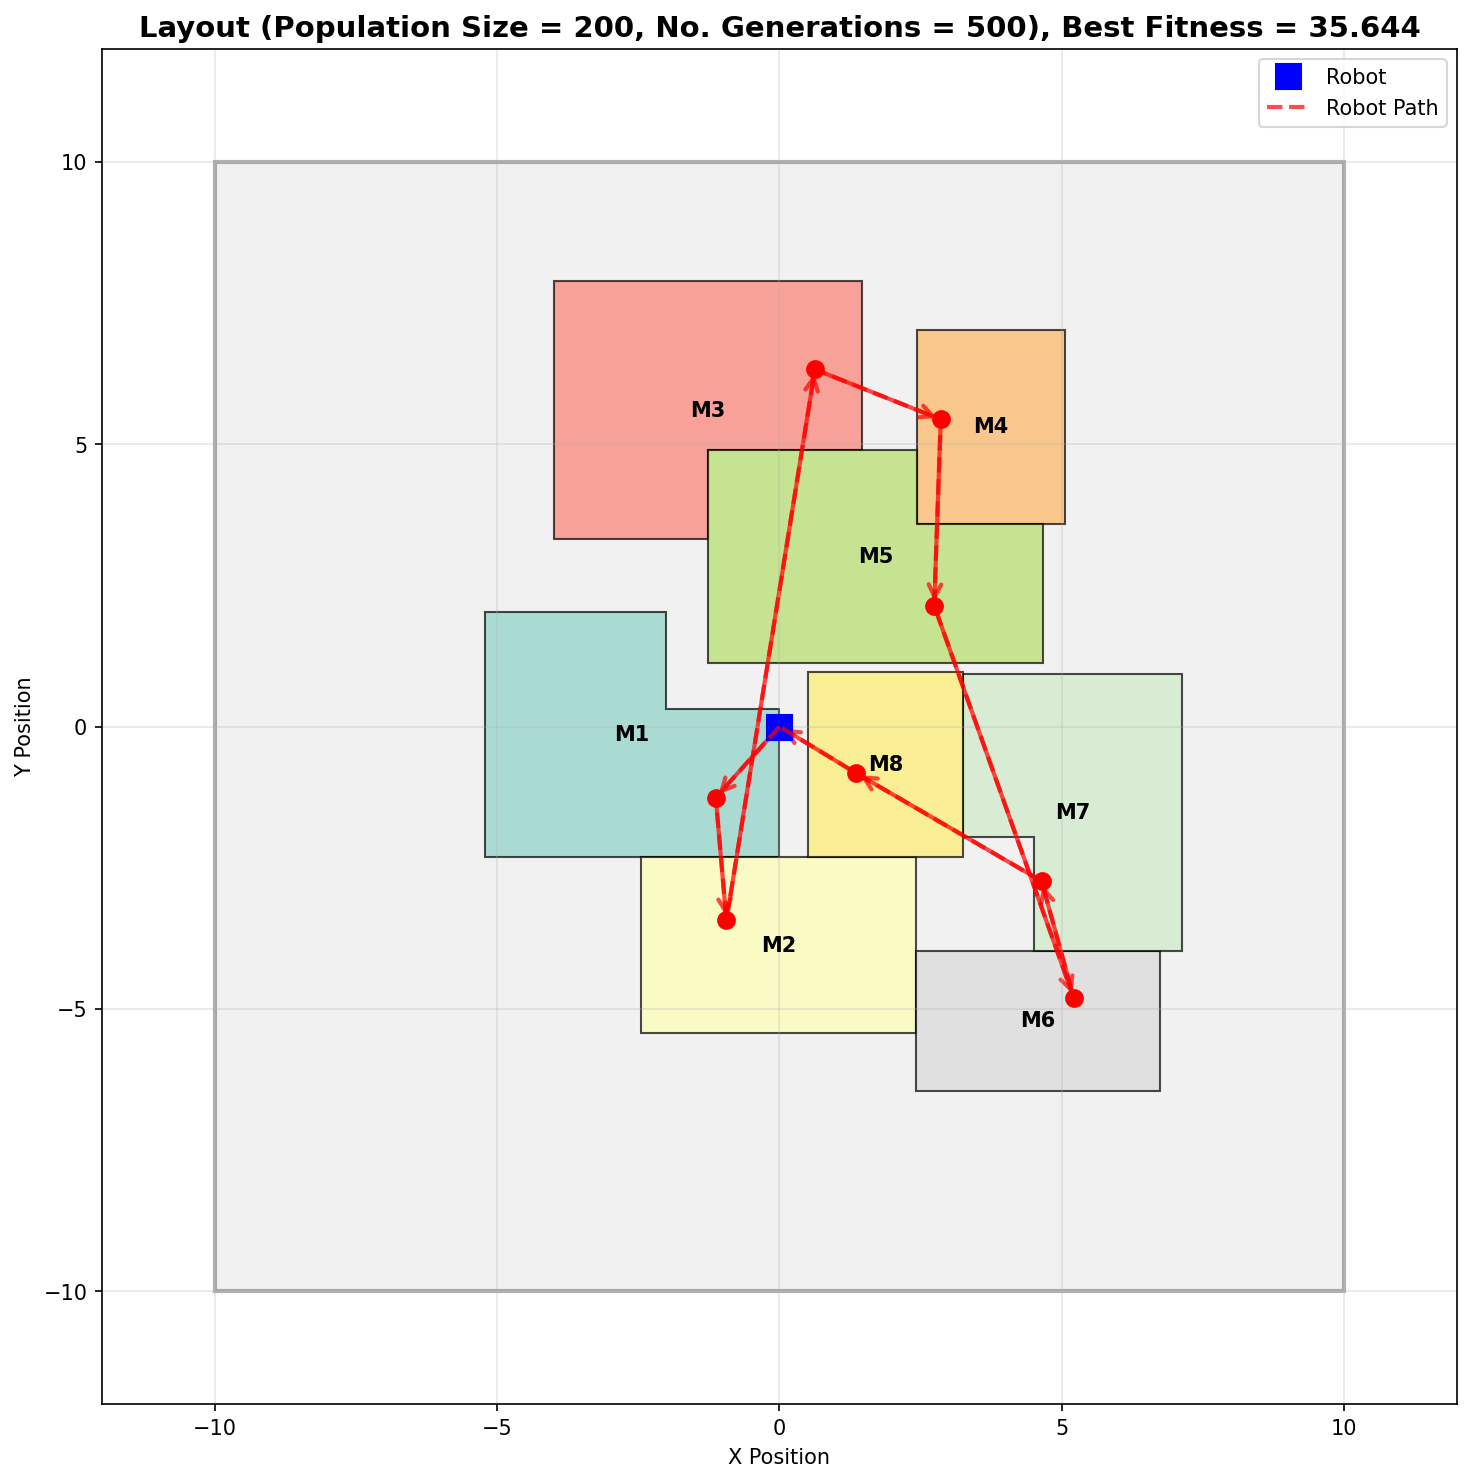
\includegraphics[width=0.7\linewidth]{ga_grid_results_incremental/pop_200/layout_pop_200_gen_500.png}
    \caption{Final optimized layout for population size 200 and 500 generations.}
\end{figure}

\clearpage

\subsubsection{Generations = 1000}
\begin{figure}[H]
    \centering
    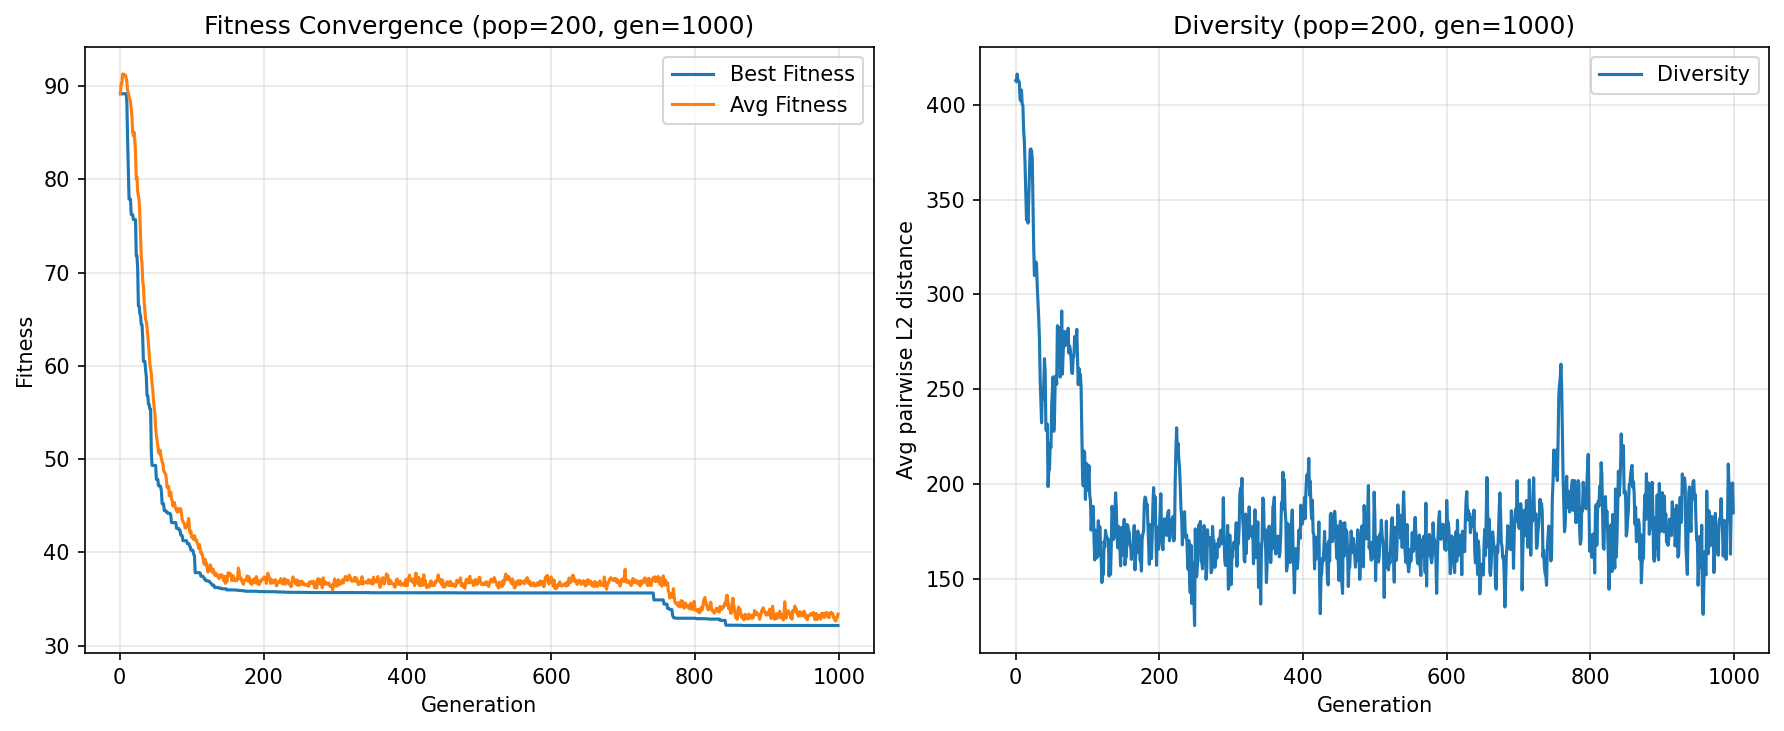
\includegraphics[width=0.9\linewidth]{ga_grid_results_incremental/pop_200/pop_200_gen_1000.png}
    \caption{Fitness convergence and diversity plot for population size 200 and 1000 generations.}
\end{figure}

\begin{figure}[H]
    \centering
    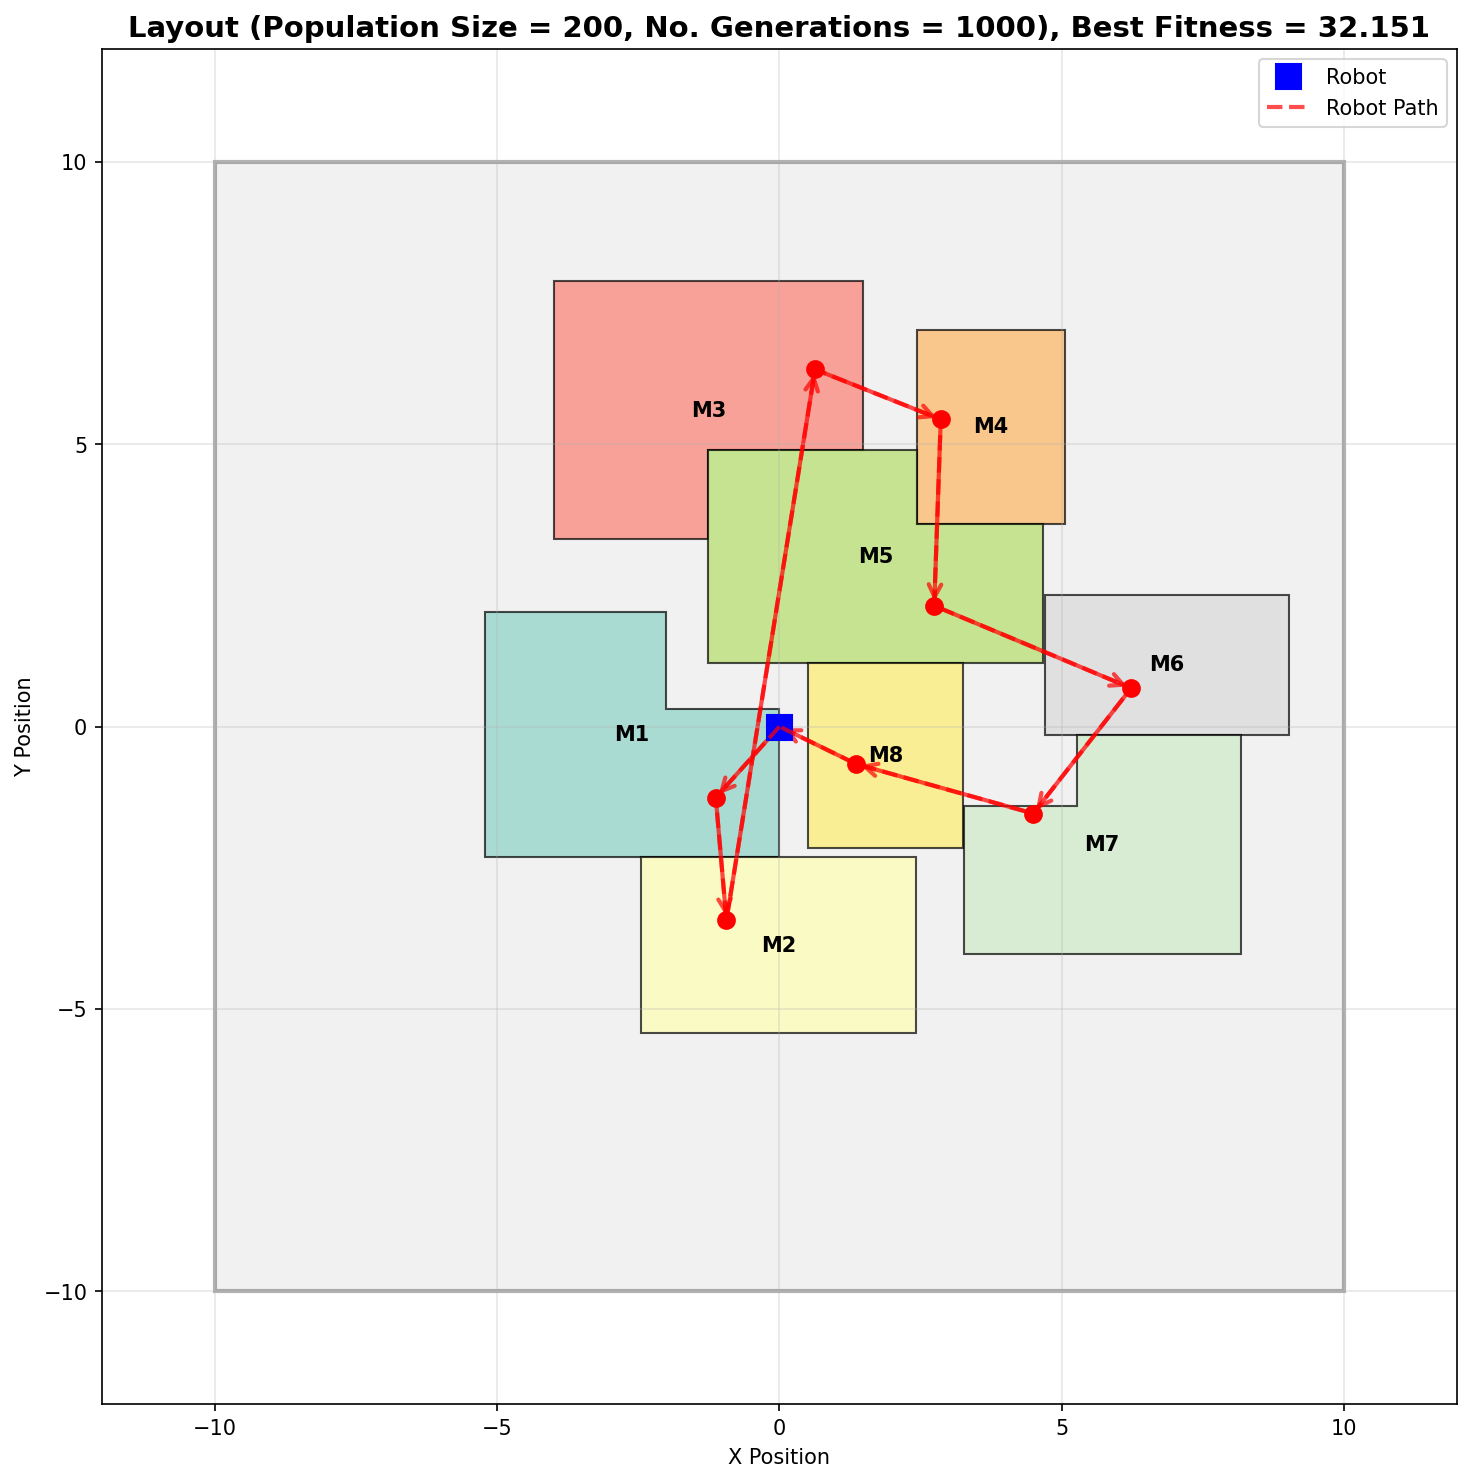
\includegraphics[width=0.7\linewidth]{ga_grid_results_incremental/pop_200/layout_pop_200_gen_1000.png}
    \caption{Final optimized layout for population size 200 and 1000 generations.}
\end{figure}

\clearpage

\subsubsection{Generations = 2000}
\begin{figure}[H]
    \centering
    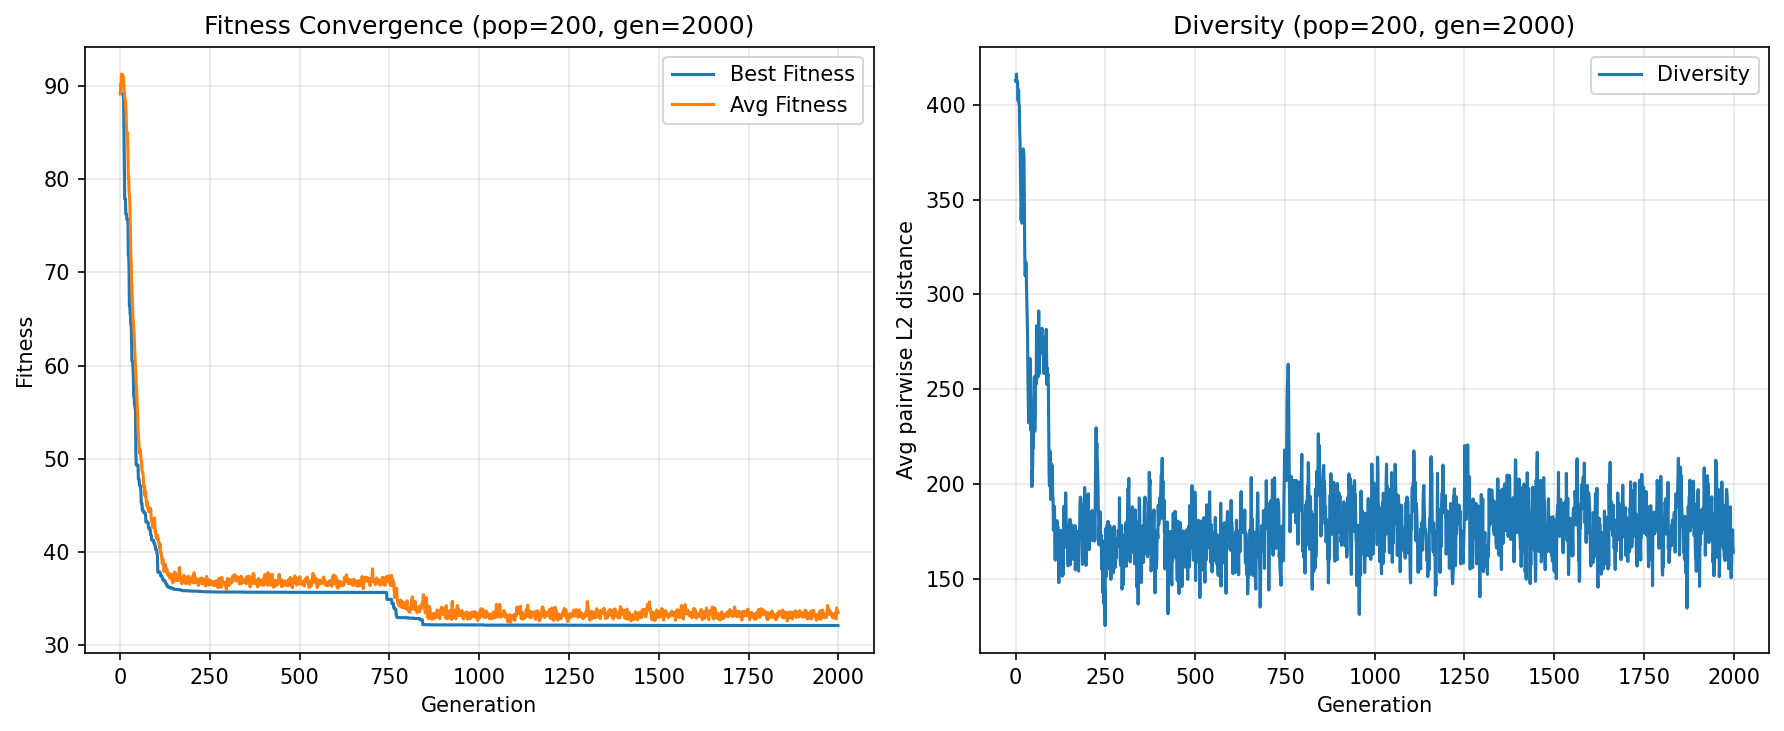
\includegraphics[width=0.9\linewidth]{ga_grid_results_incremental/pop_200/pop_200_gen_2000.png}
    \caption{Fitness convergence and diversity plot for population size 200 and 2000 generations.}
\end{figure}

\begin{figure}[H]
    \centering
    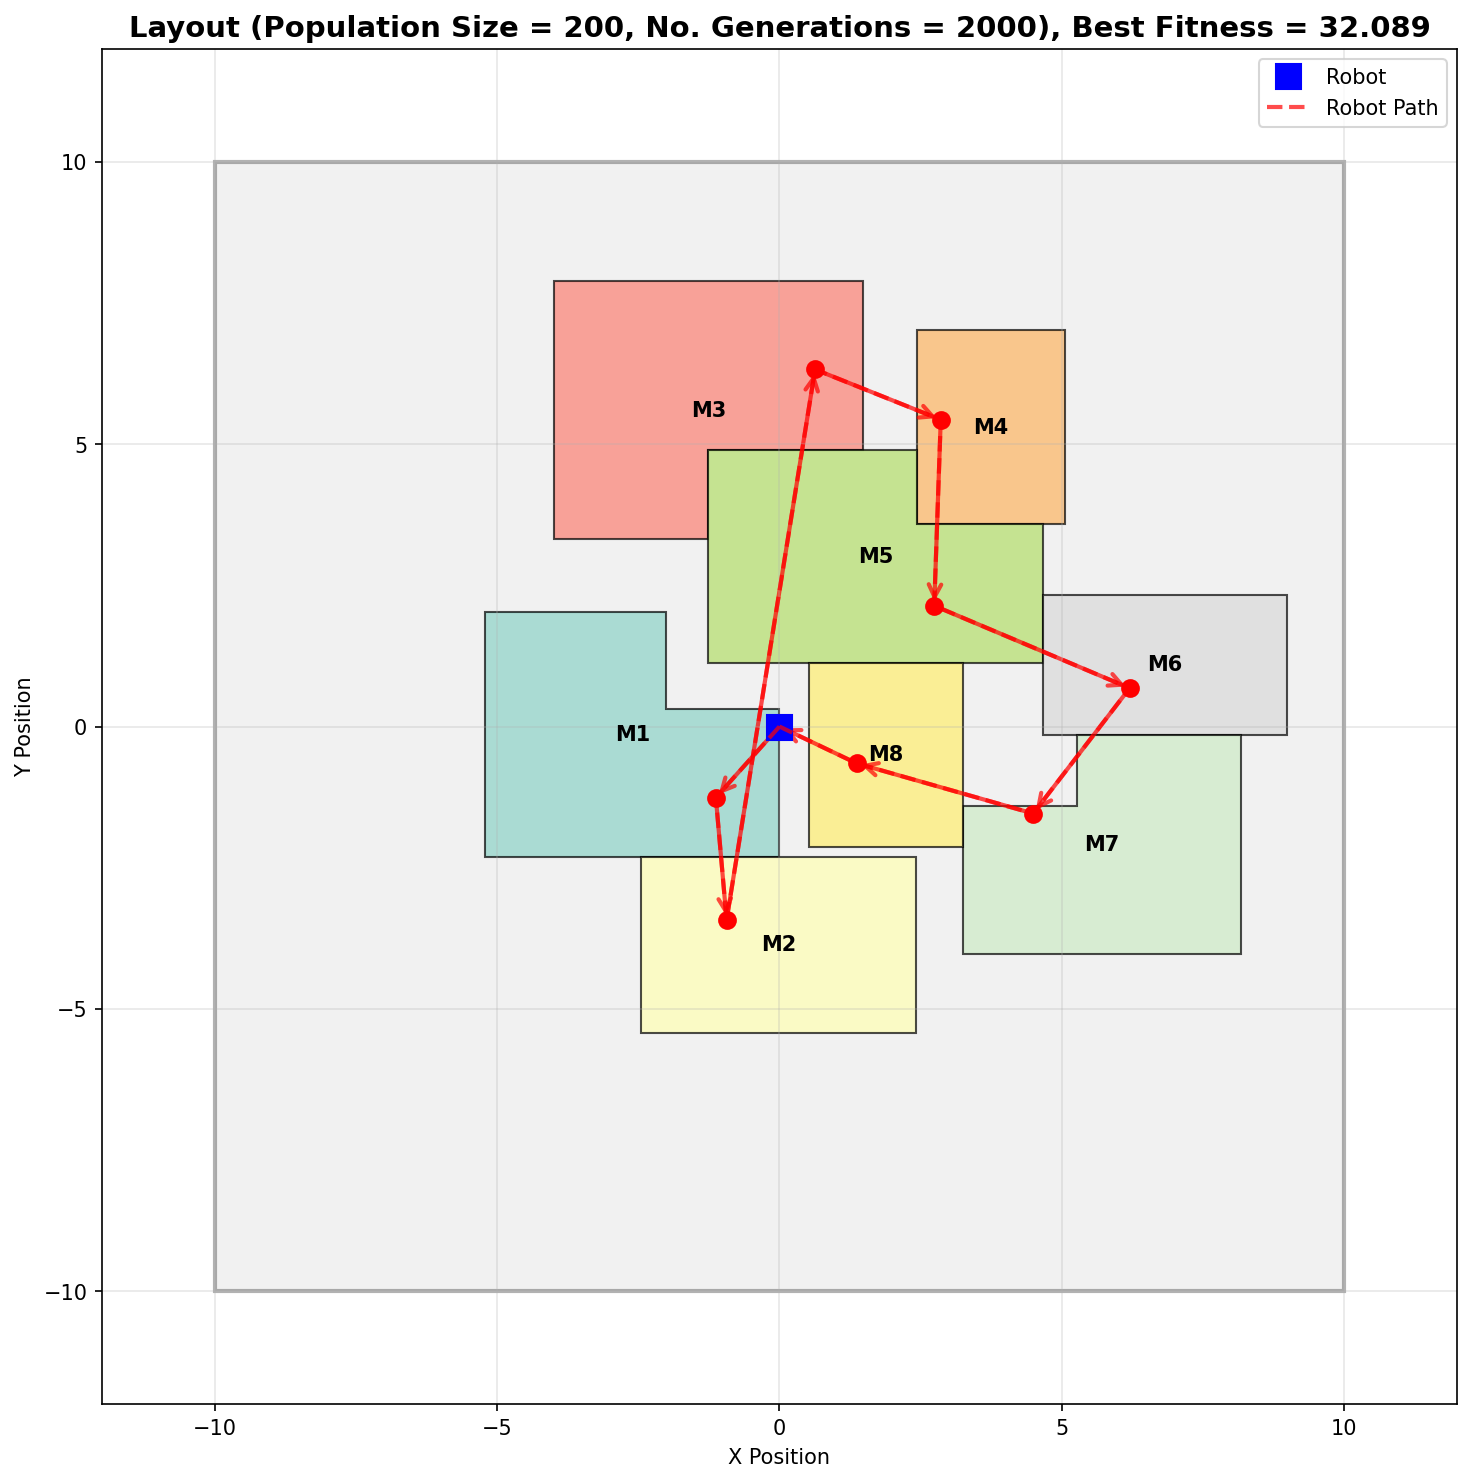
\includegraphics[width=0.7\linewidth]{ga_grid_results_incremental/pop_200/layout_pop_200_gen_2000.png}
    \caption{Final optimized layout for population size 200 and 2000 generations.}
\end{figure}

\clearpage

%====================================================
\subsection{Population Size = 500}
%====================================================

\subsubsection{Generations = 100}
\begin{figure}[H]
    \centering
    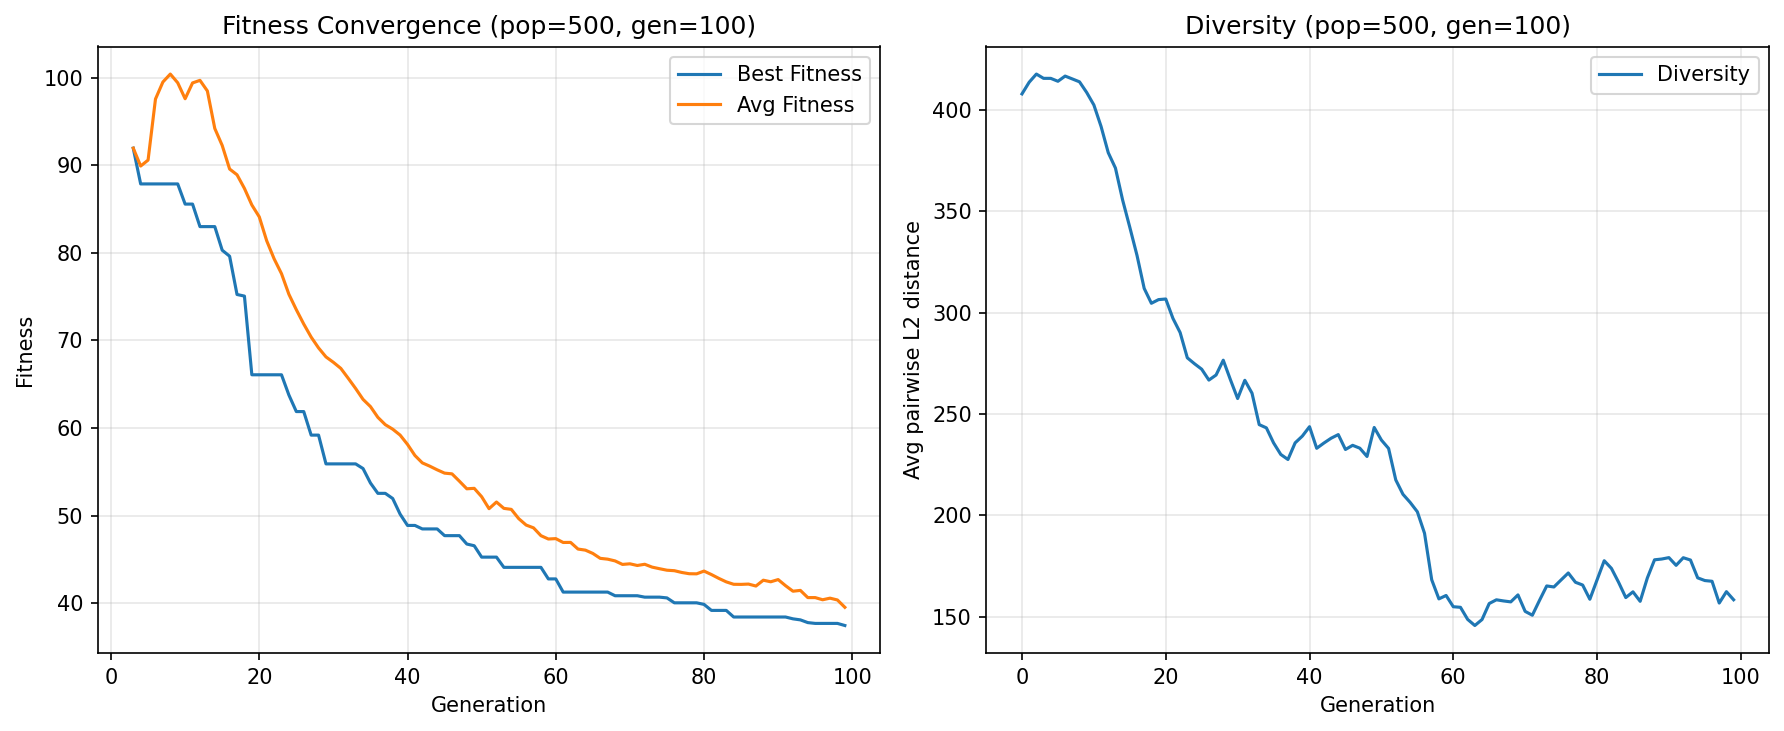
\includegraphics[width=0.9\linewidth]{ga_grid_results_incremental/pop_500/pop_500_gen_100.png}
    \caption{Fitness convergence and diversity plot for population size 500 and 100 generations.}
\end{figure}

\begin{figure}[H]
    \centering
    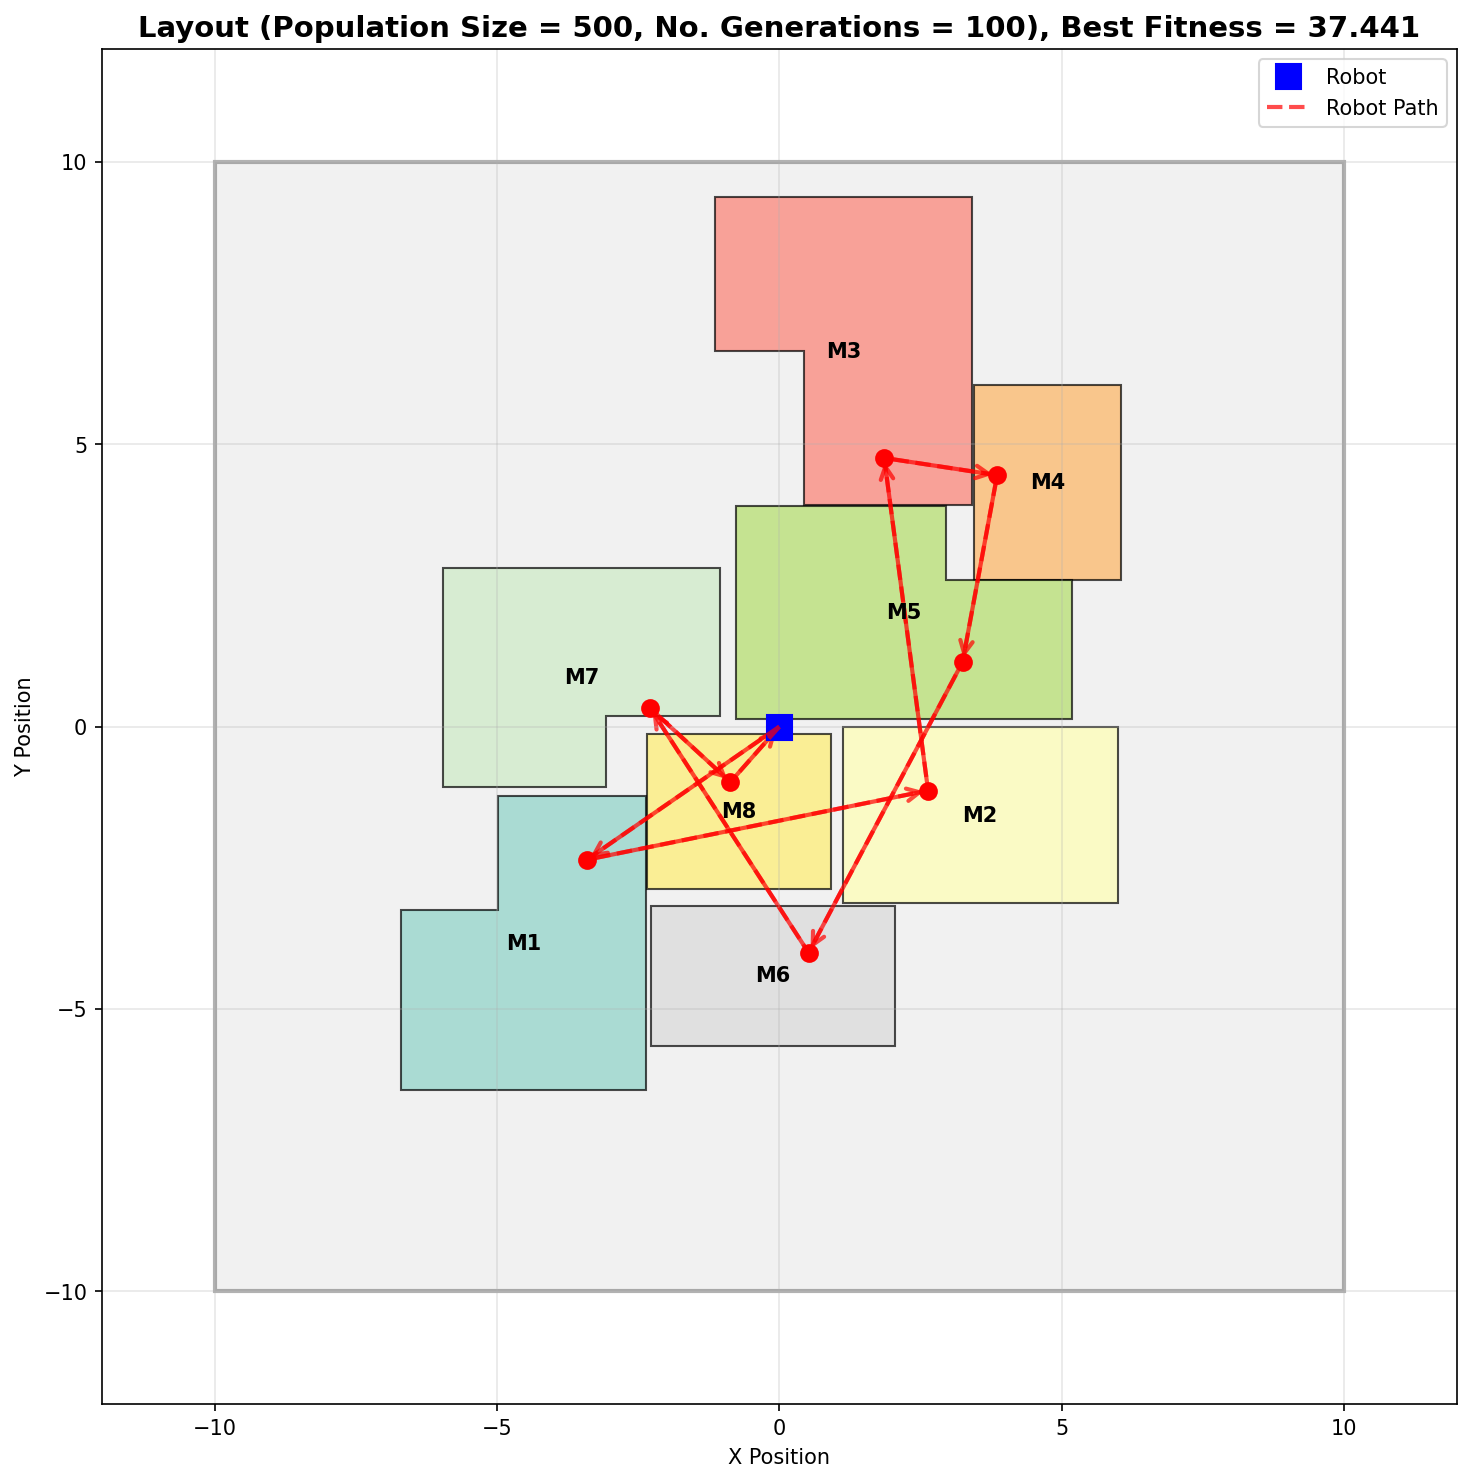
\includegraphics[width=0.7\linewidth]{ga_grid_results_incremental/pop_500/layout_pop_500_gen_100.png}
    \caption{Final optimized layout for population size 500 and 100 generations.}
\end{figure}

\clearpage

\subsubsection{Generations = 200}
\begin{figure}[H]
    \centering
    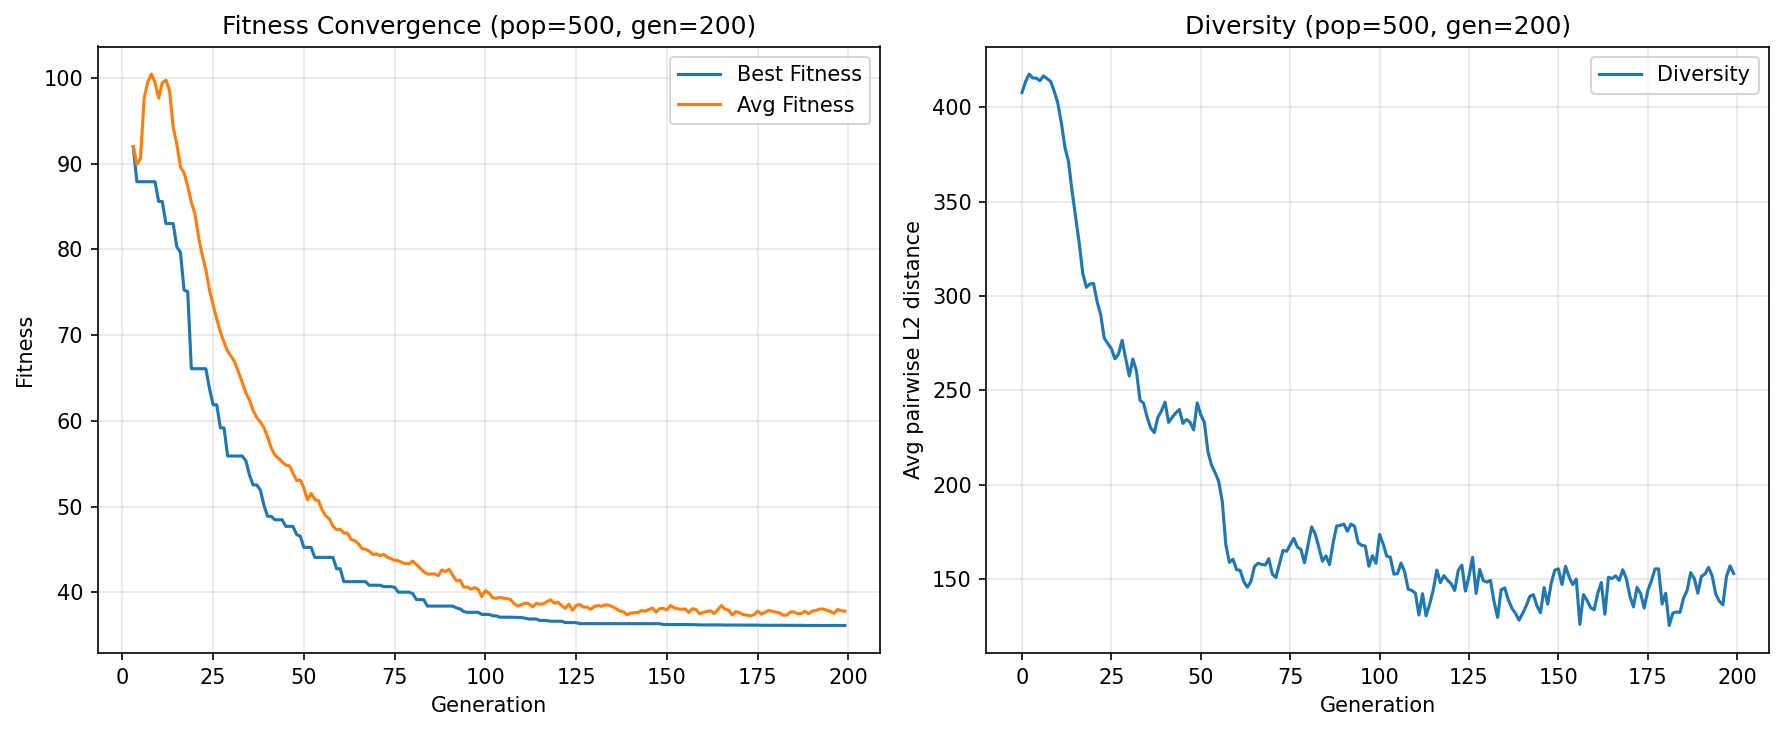
\includegraphics[width=0.9\linewidth]{ga_grid_results_incremental/pop_500/pop_500_gen_200.png}
    \caption{Fitness convergence and diversity plot for population size 500 and 200 generations.}
\end{figure}

\begin{figure}[H]
    \centering
    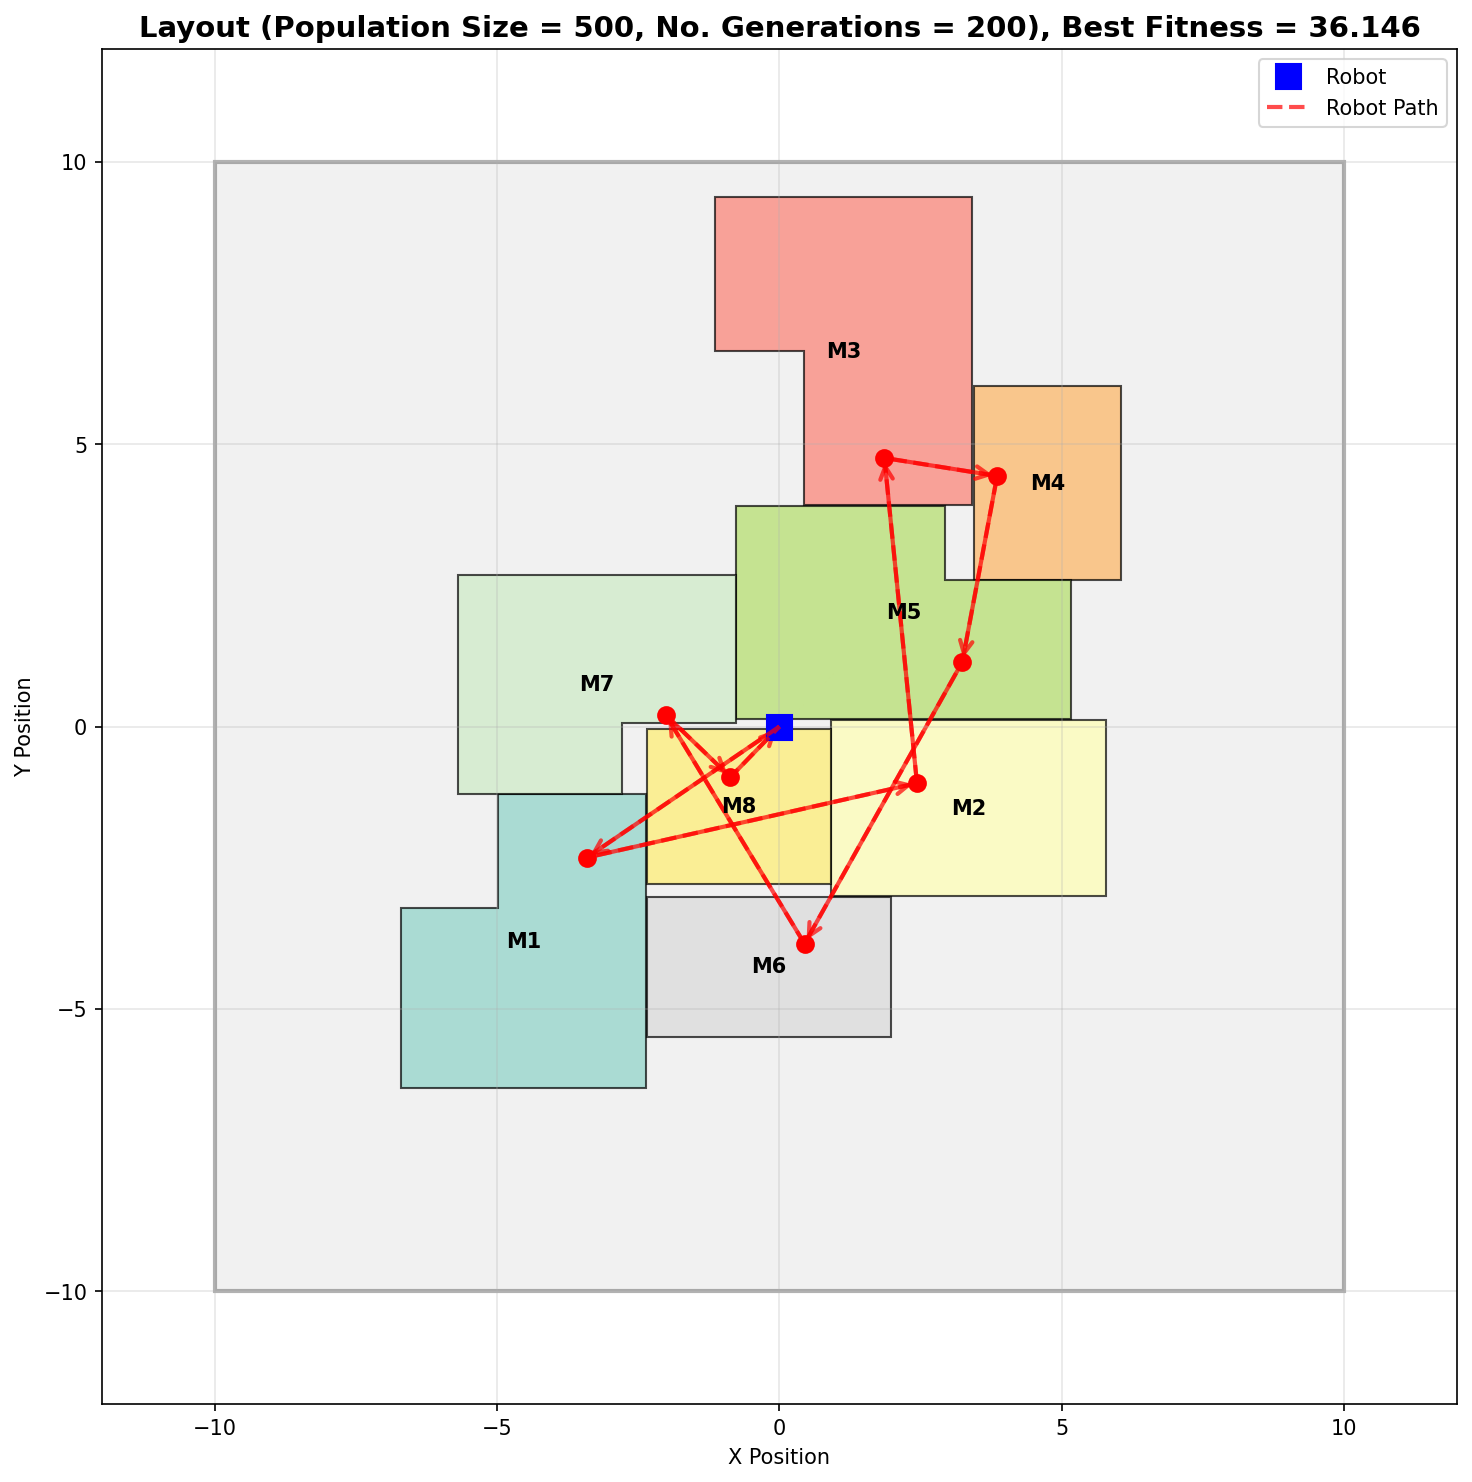
\includegraphics[width=0.7\linewidth]{ga_grid_results_incremental/pop_500/layout_pop_500_gen_200.png}
    \caption{Final optimized layout for population size 500 and 200 generations.}
\end{figure}

\clearpage

\subsubsection{Generations = 500}
\begin{figure}[H]
    \centering
    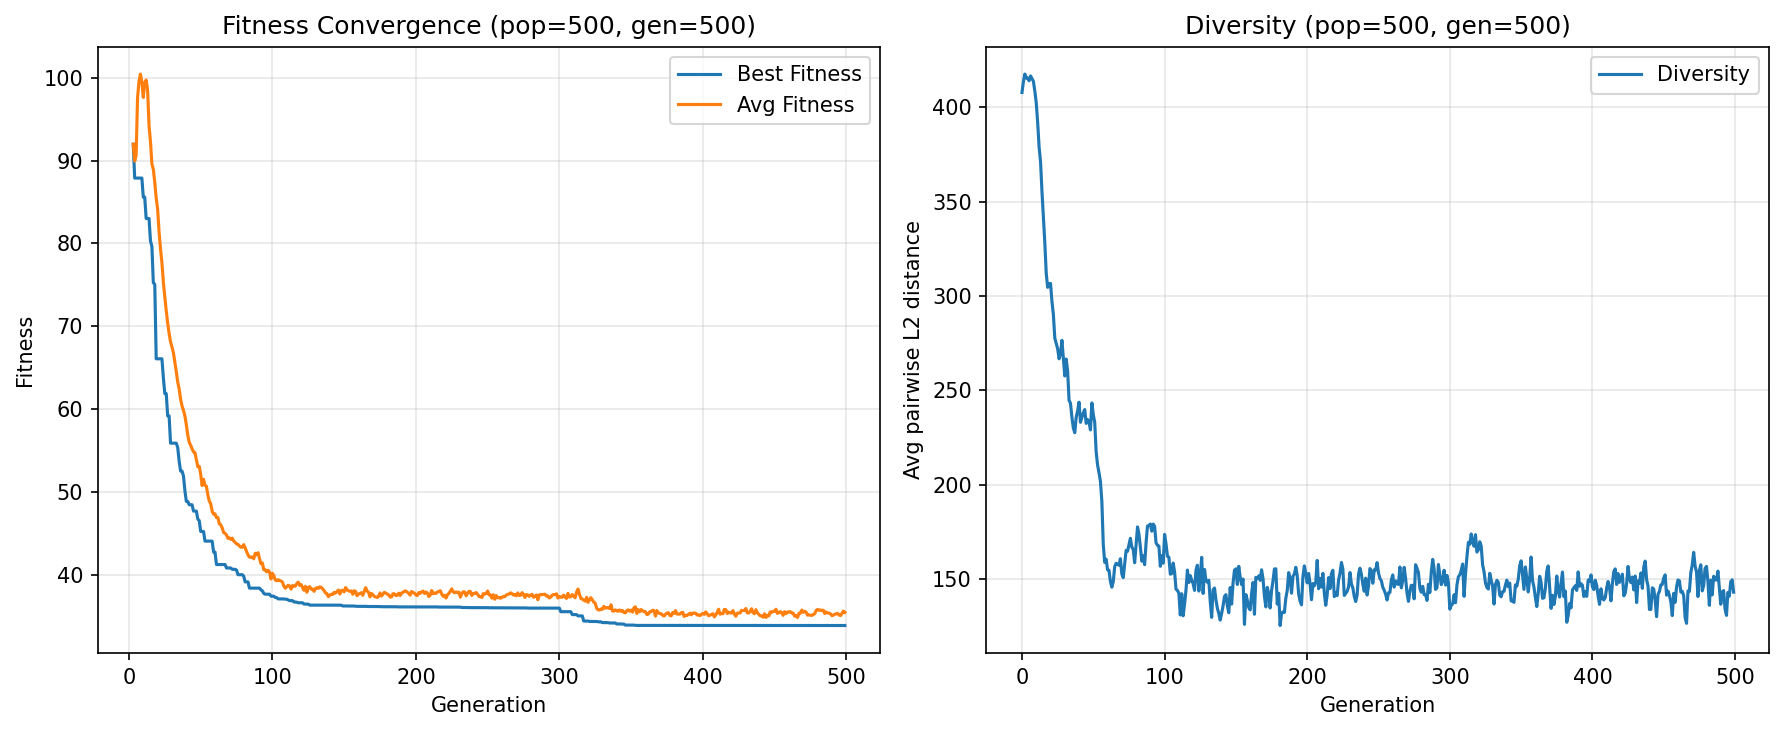
\includegraphics[width=0.9\linewidth]{ga_grid_results_incremental/pop_500/pop_500_gen_500.png}
    \caption{Fitness convergence and diversity plot for population size 500 and 500 generations.}
\end{figure}

\begin{figure}[H]
    \centering
    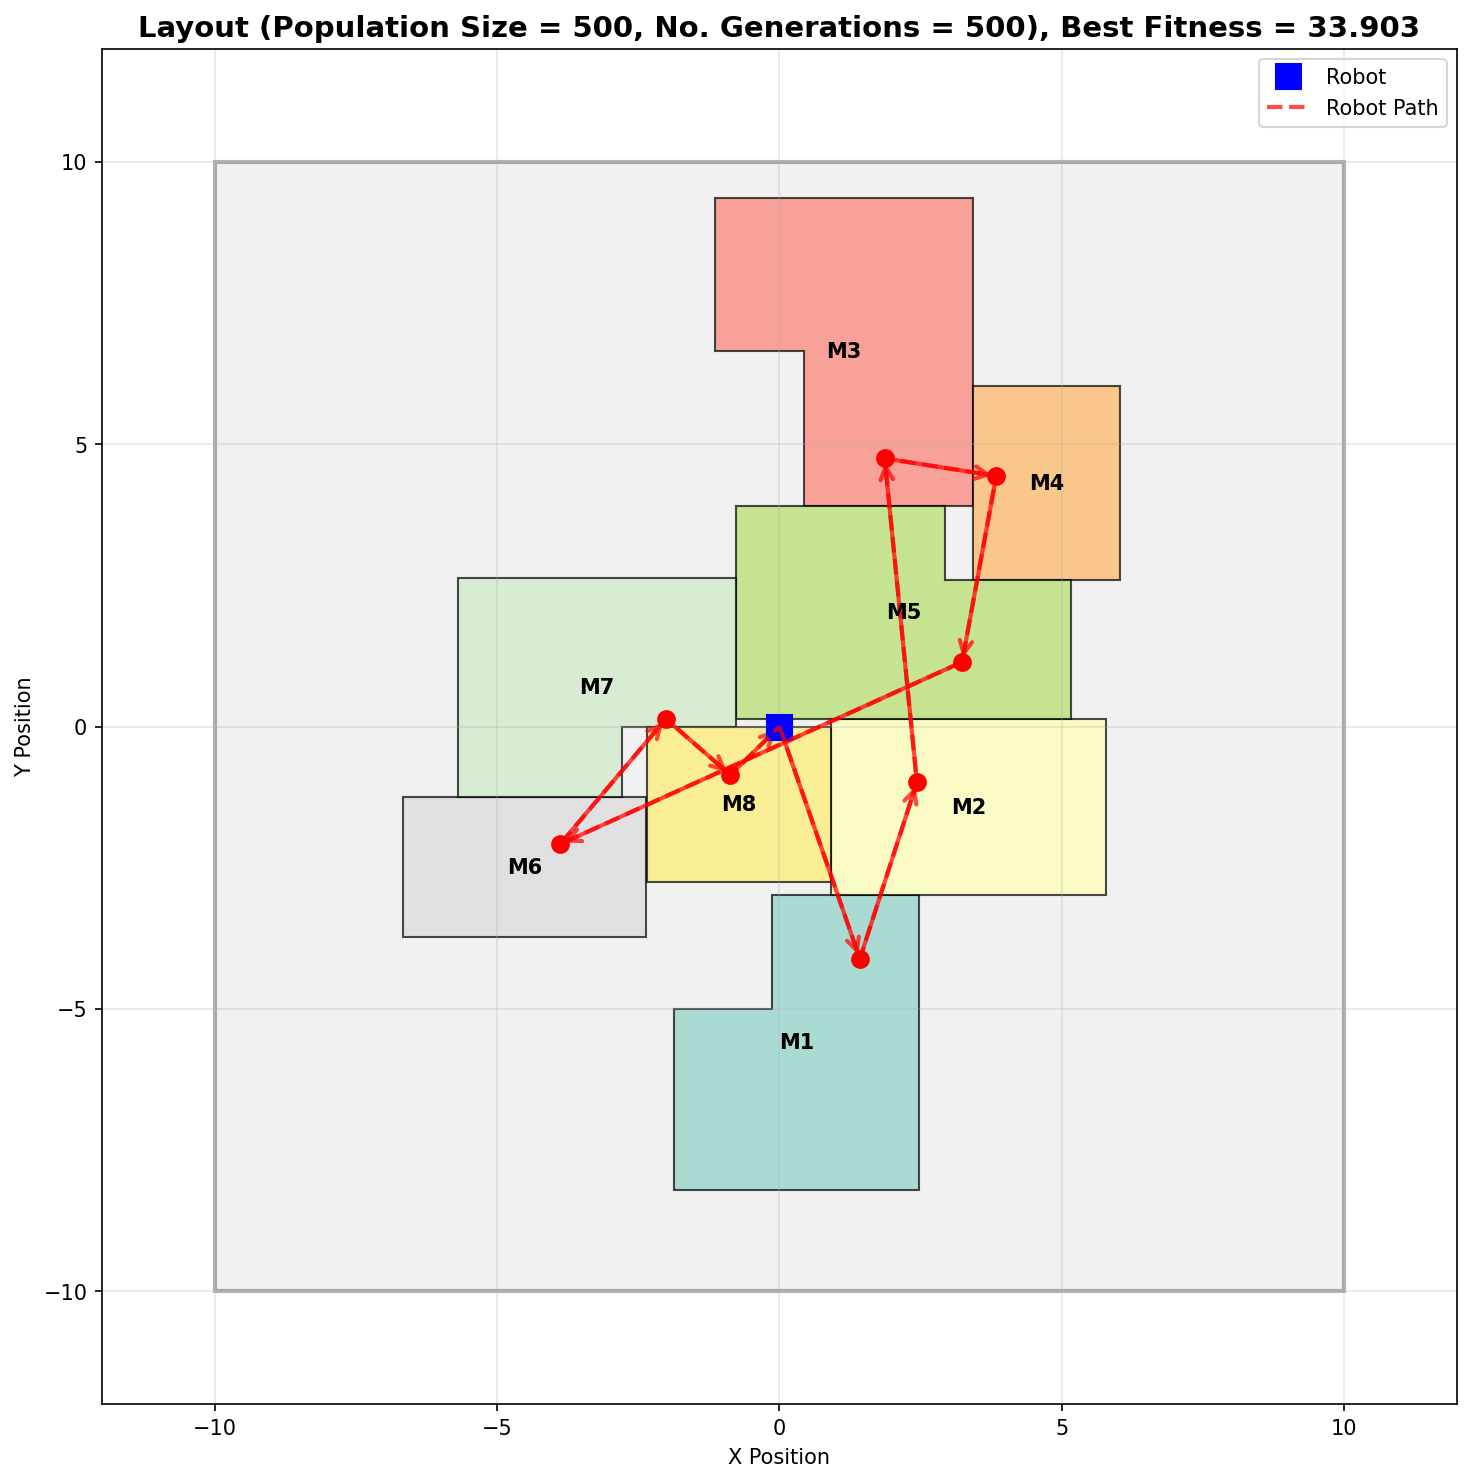
\includegraphics[width=0.7\linewidth]{ga_grid_results_incremental/pop_500/layout_pop_500_gen_500.png}
    \caption{Final optimized layout for population size 500 and 500 generations.}
\end{figure}

\clearpage

\subsubsection{Generations = 1000}
\begin{figure}[H]
    \centering
    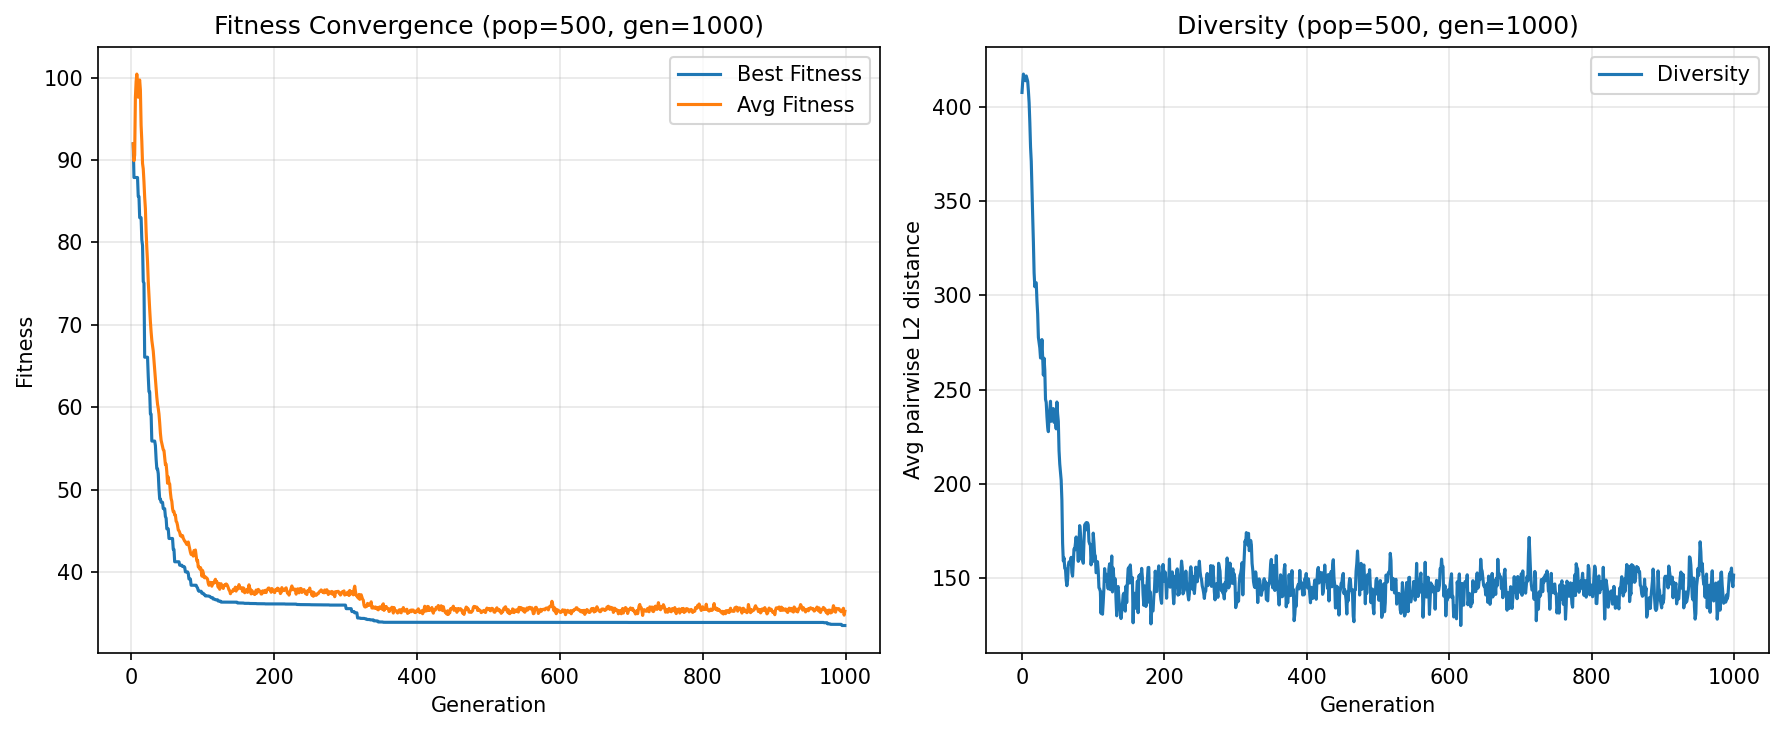
\includegraphics[width=0.9\linewidth]{ga_grid_results_incremental/pop_500/pop_500_gen_1000.png}
    \caption{Fitness convergence and diversity plot for population size 500 and 1000 generations.}
\end{figure}

\begin{figure}[H]
    \centering
    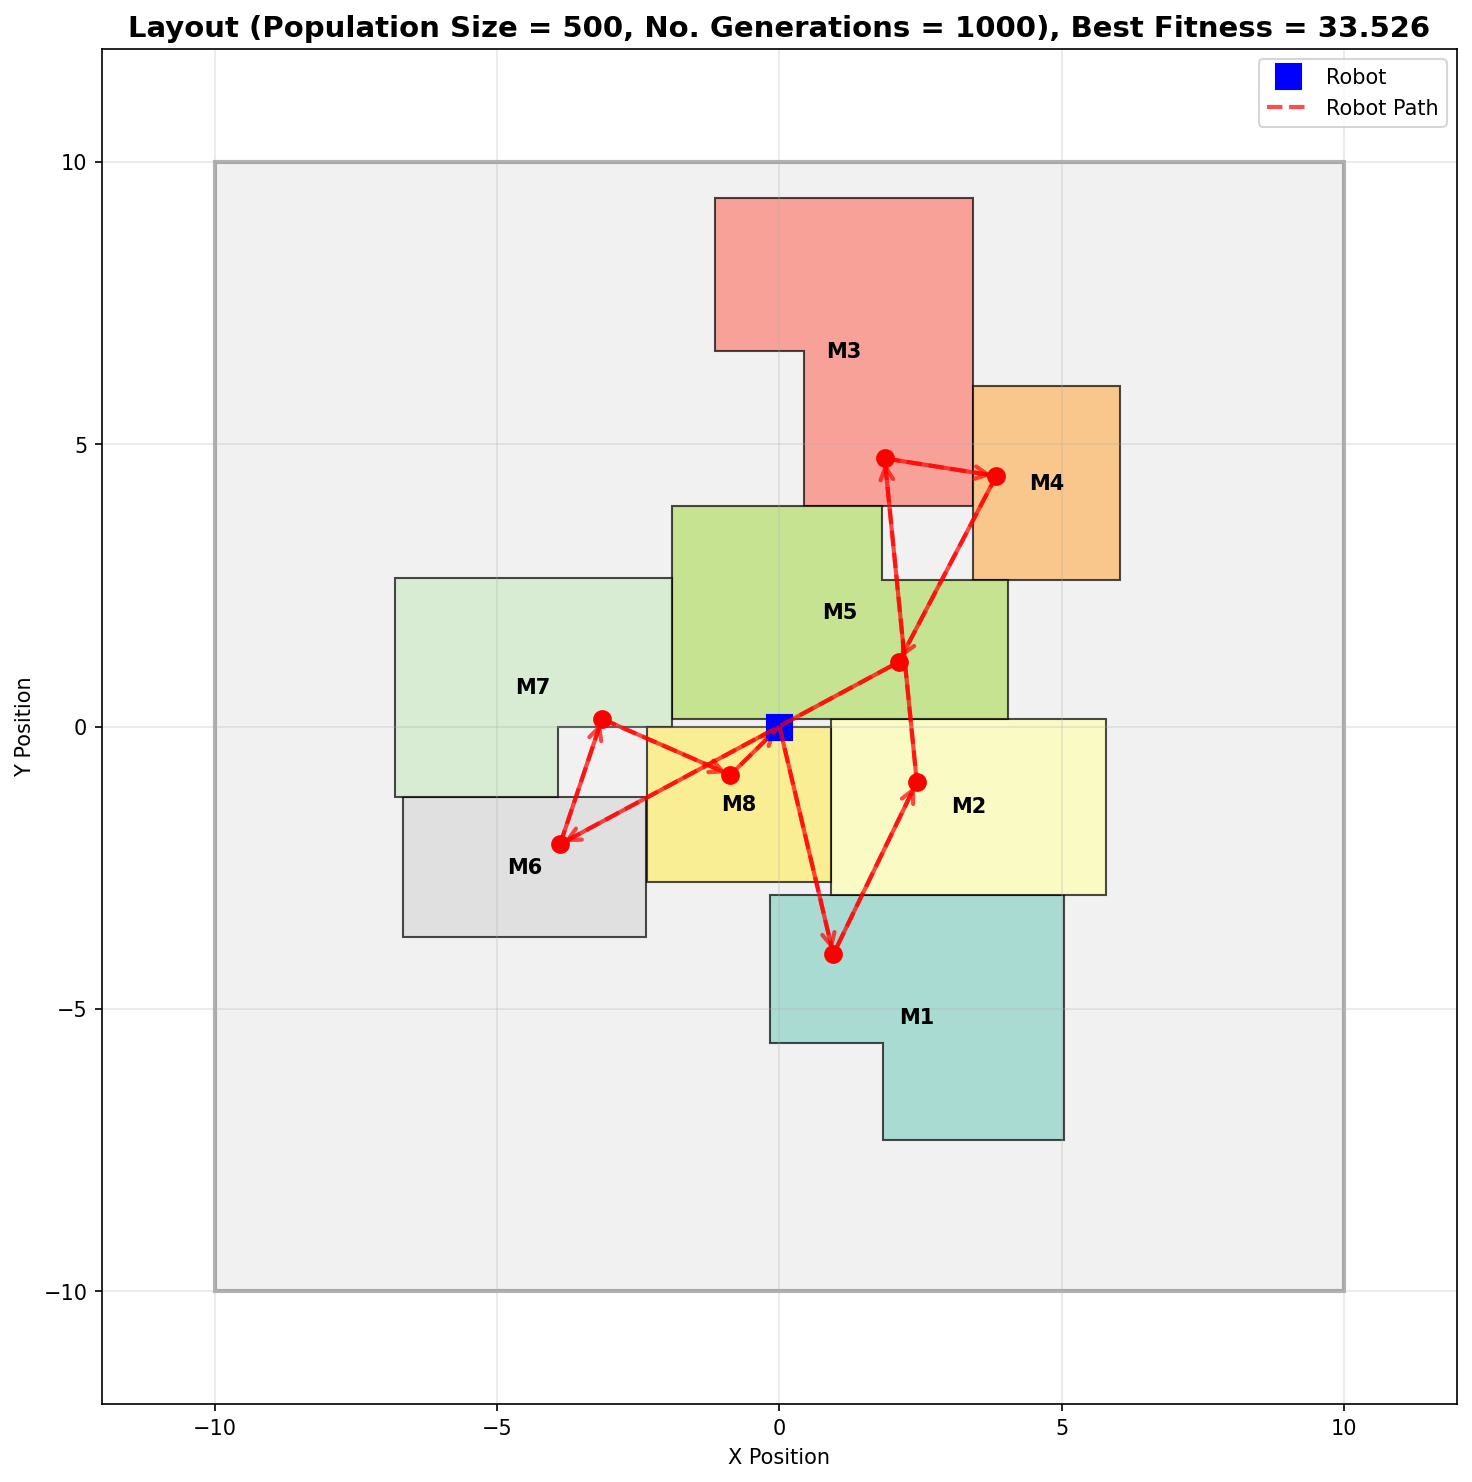
\includegraphics[width=0.7\linewidth]{ga_grid_results_incremental/pop_500/layout_pop_500_gen_1000.png}
    \caption{Final optimized layout for population size 500 and 1000 generations.}
\end{figure}

\clearpage

\subsubsection{Generations = 2000}
\begin{figure}[H]
    \centering
    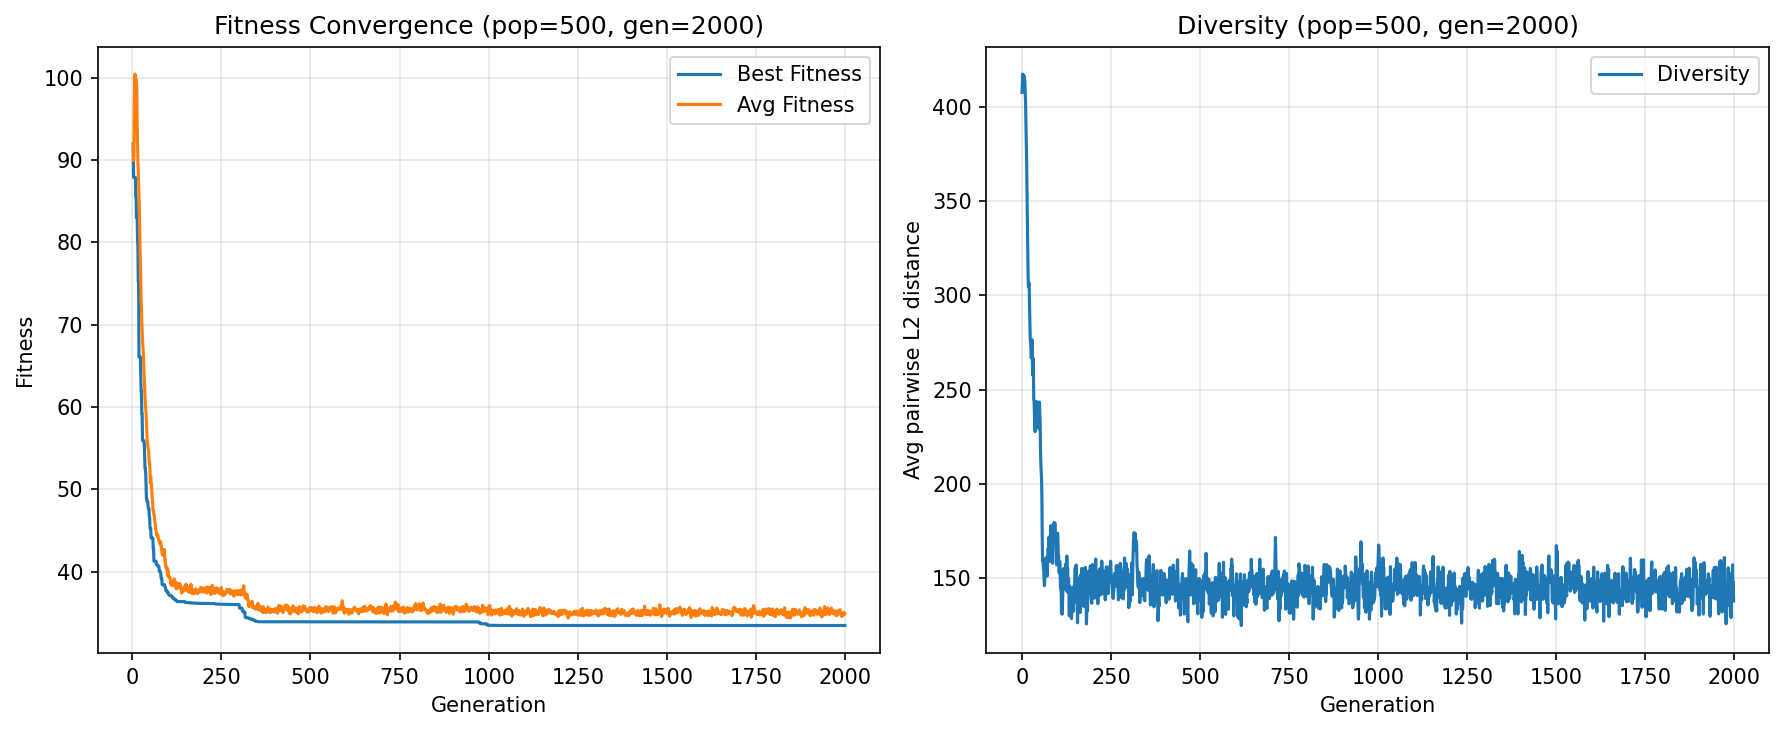
\includegraphics[width=0.9\linewidth]{ga_grid_results_incremental/pop_500/pop_500_gen_2000.png}
    \caption{Fitness convergence and diversity plot for population size 500 and 2000 generations.}
\end{figure}

\begin{figure}[H]
    \centering
    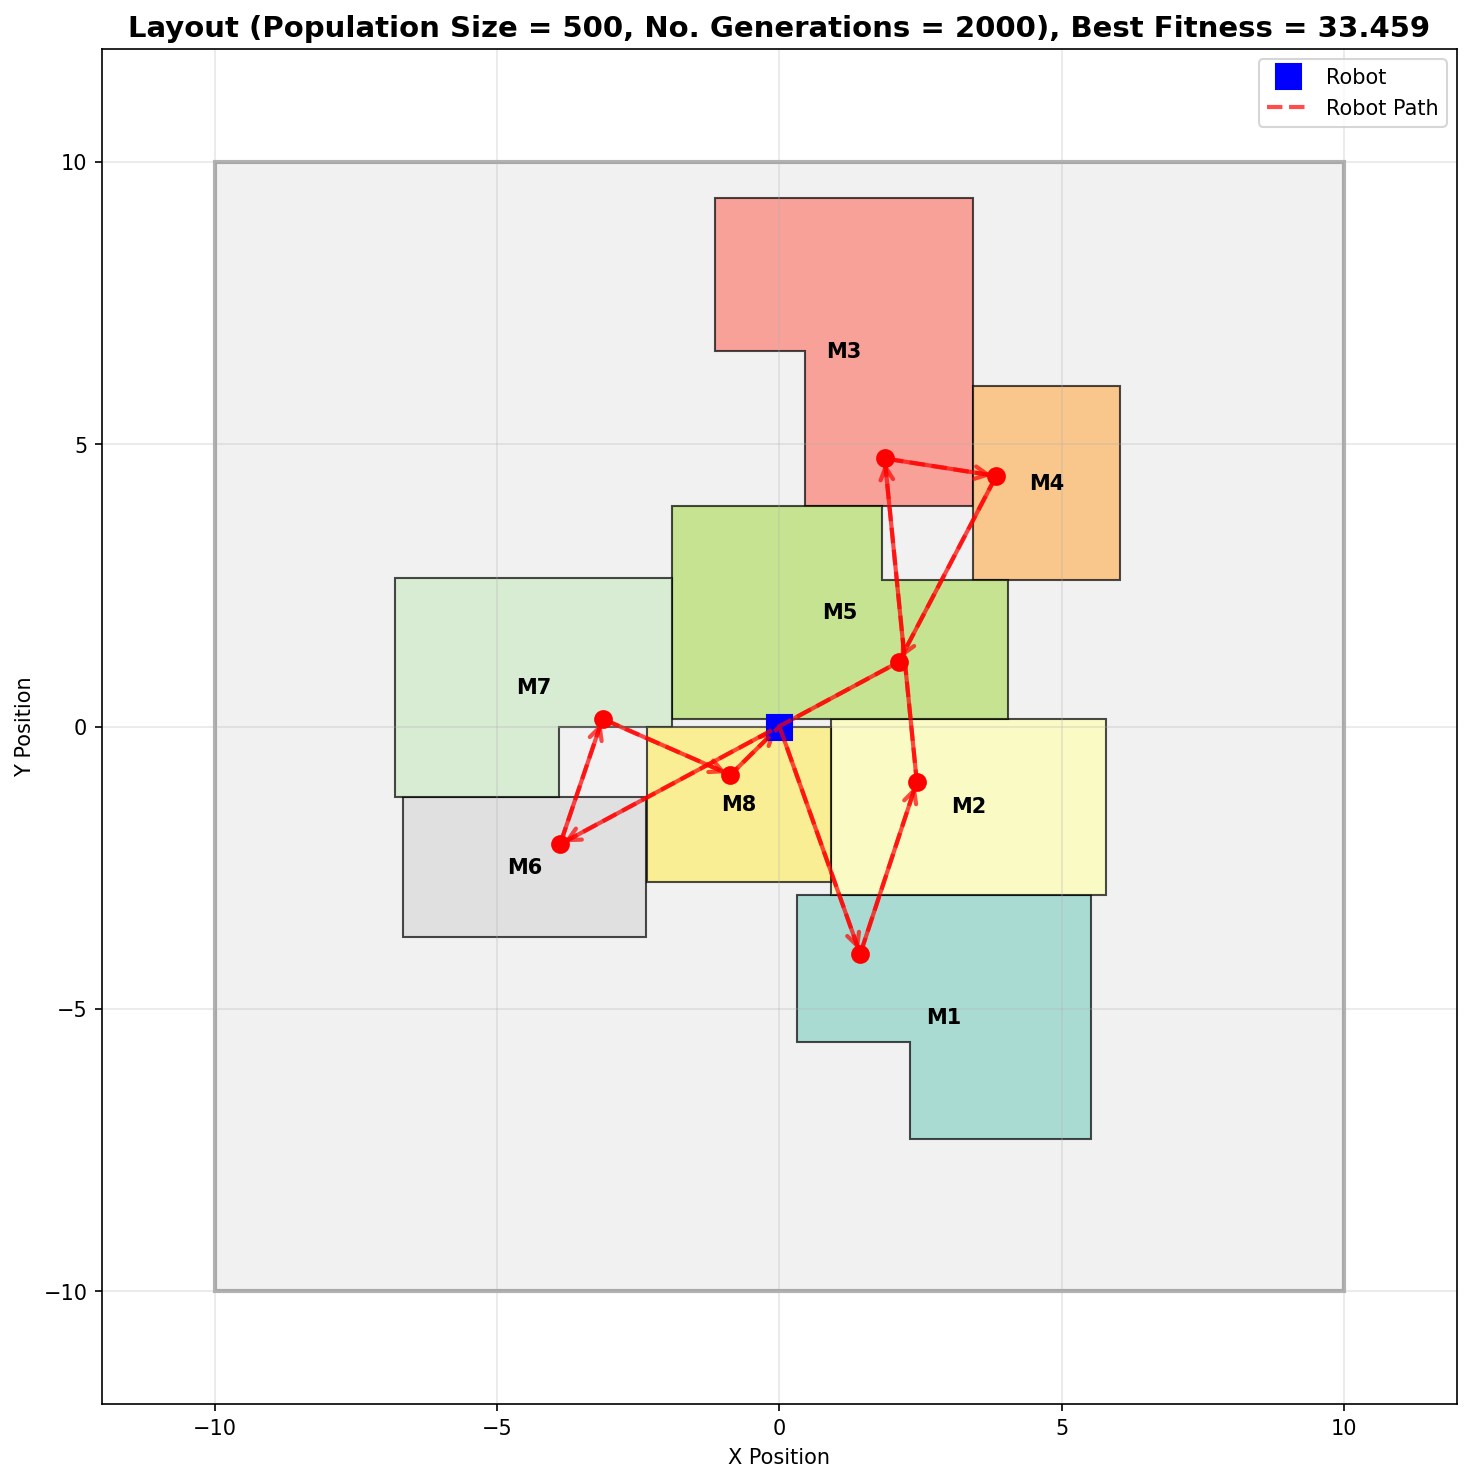
\includegraphics[width=0.7\linewidth]{ga_grid_results_incremental/pop_500/layout_pop_500_gen_2000.png}
    \caption{Final optimized layout for population size 500 and 2000 generations.}
\end{figure}

\clearpage

%====================================================
\subsection{Population Size = 1000}
%====================================================

\subsubsection{Generations = 100}
\begin{figure}[H]
    \centering
    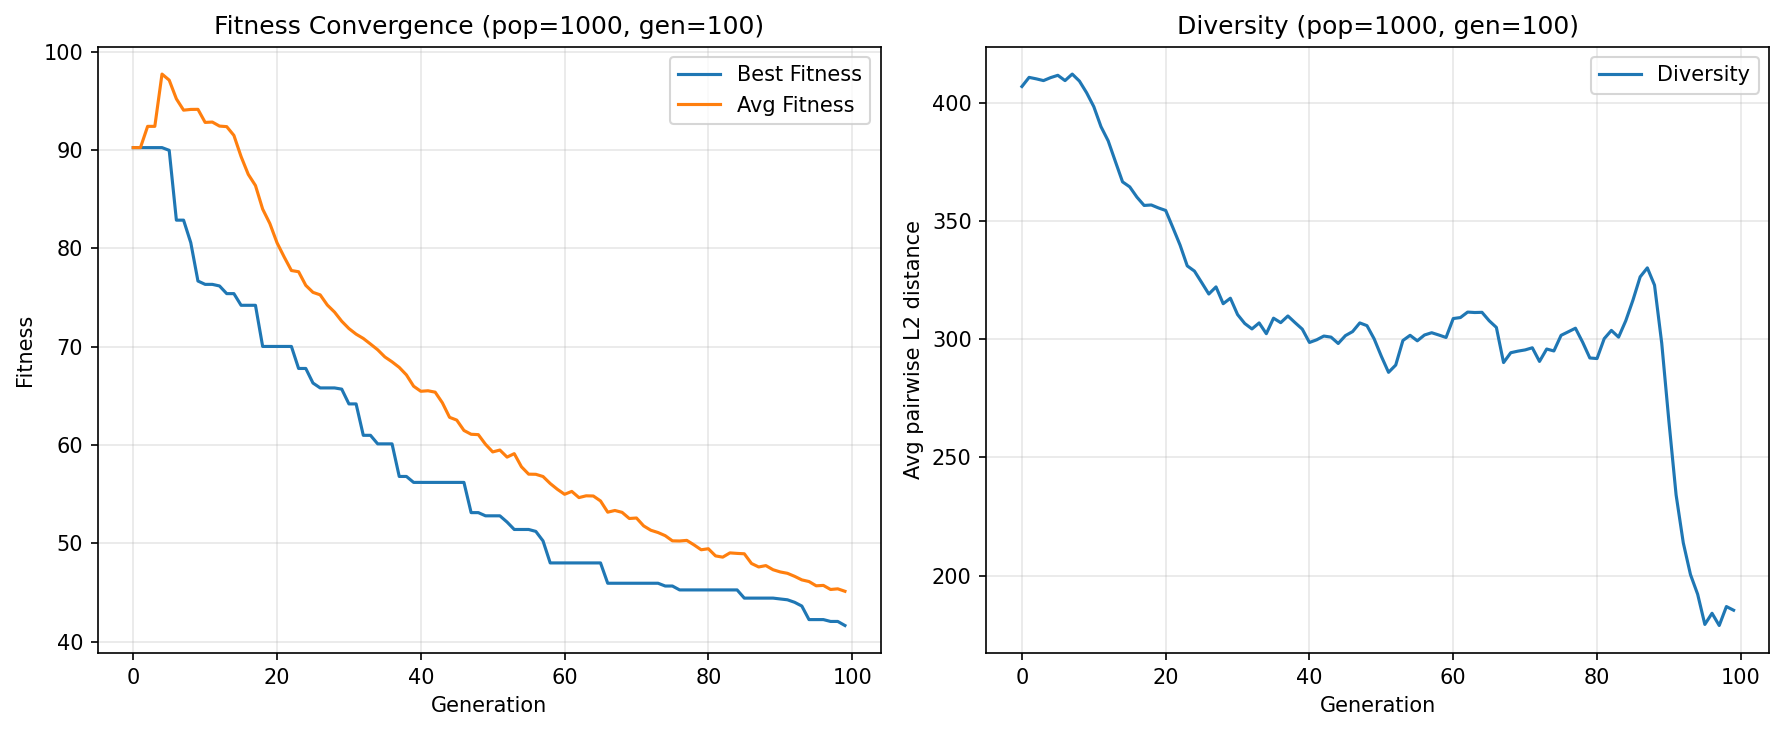
\includegraphics[width=0.9\linewidth]{ga_grid_results_incremental/pop_1000/pop_1000_gen_100.png}
    \caption{Fitness convergence and diversity plot for population size 1000 and 100 generations.}
\end{figure}

\begin{figure}[H]
    \centering
    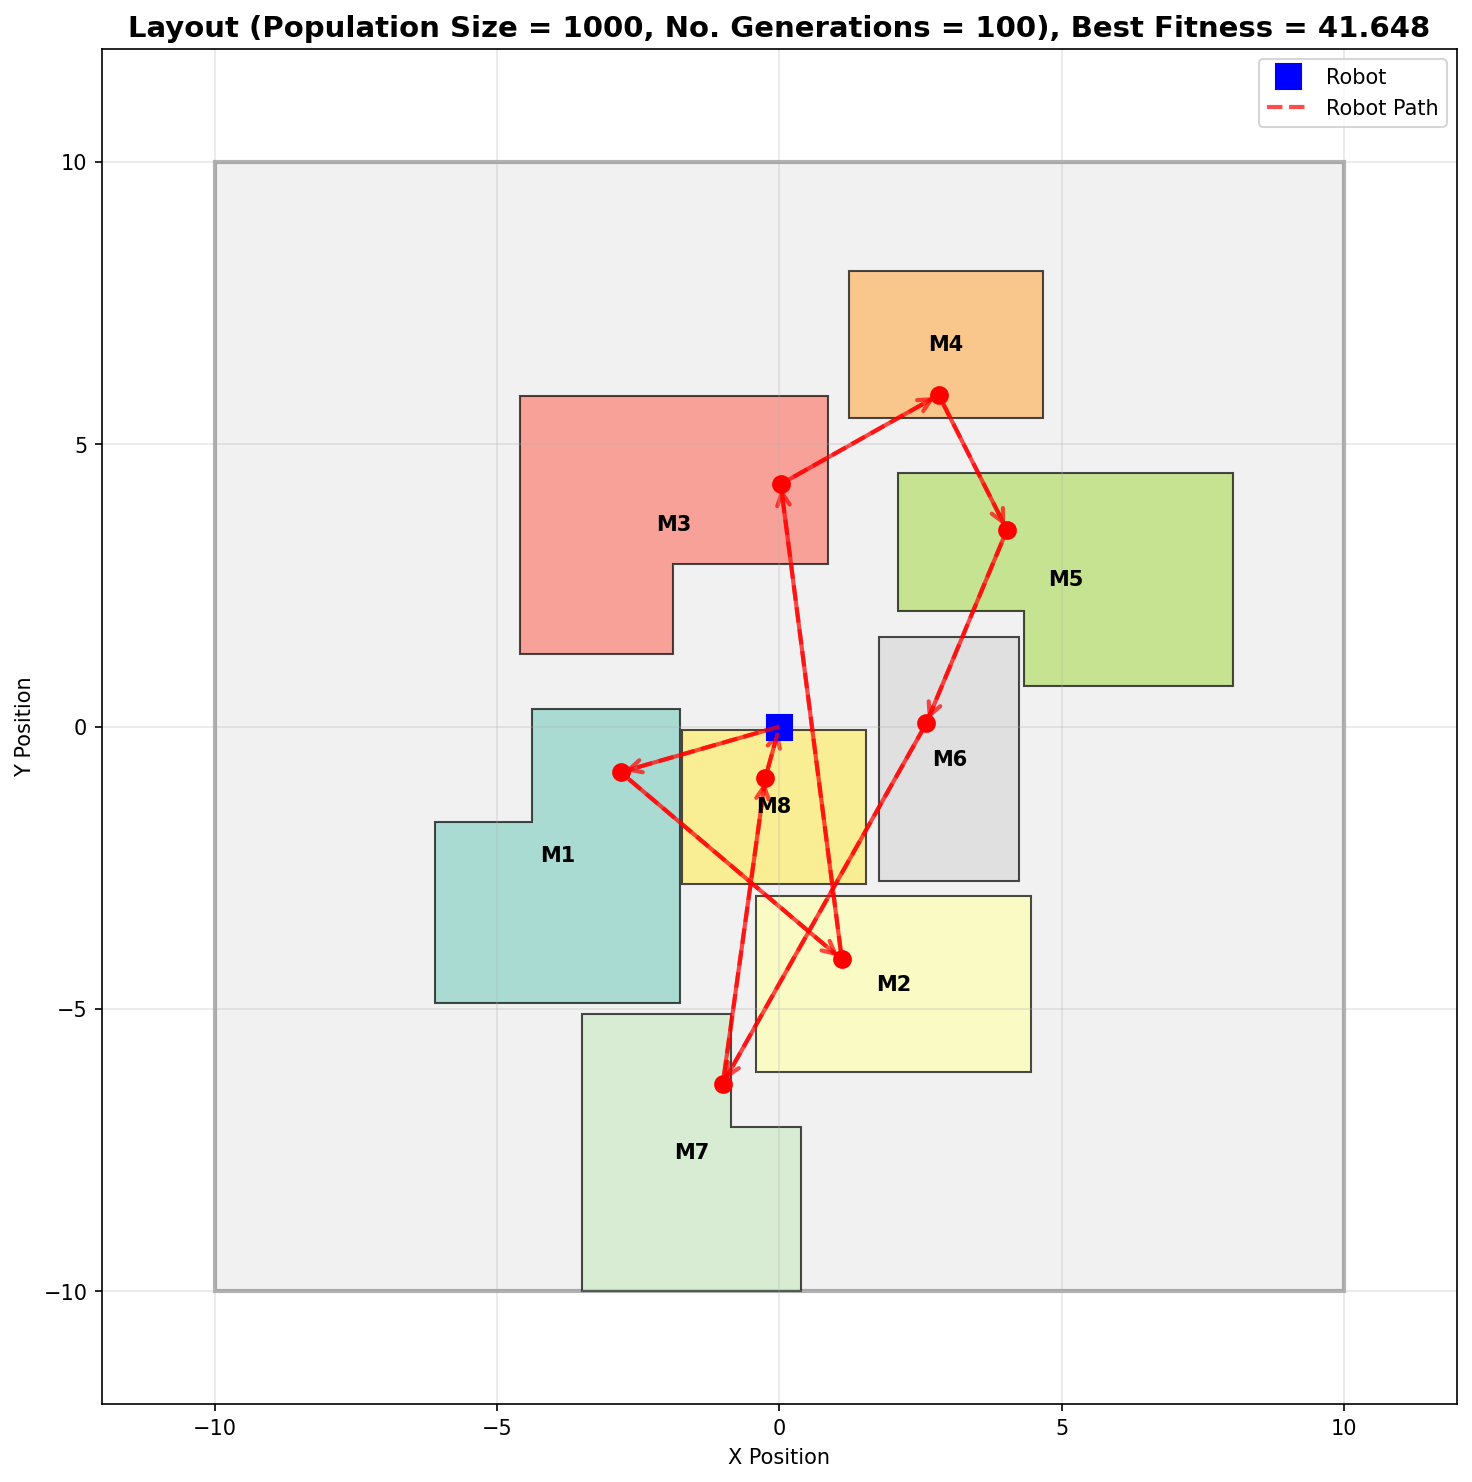
\includegraphics[width=0.7\linewidth]{ga_grid_results_incremental/pop_1000/layout_pop_1000_gen_100.png}
    \caption{Final optimized layout for population size 1000 and 100 generations.}
\end{figure}

\clearpage

\subsubsection{Generations = 200}
\begin{figure}[H]
    \centering
    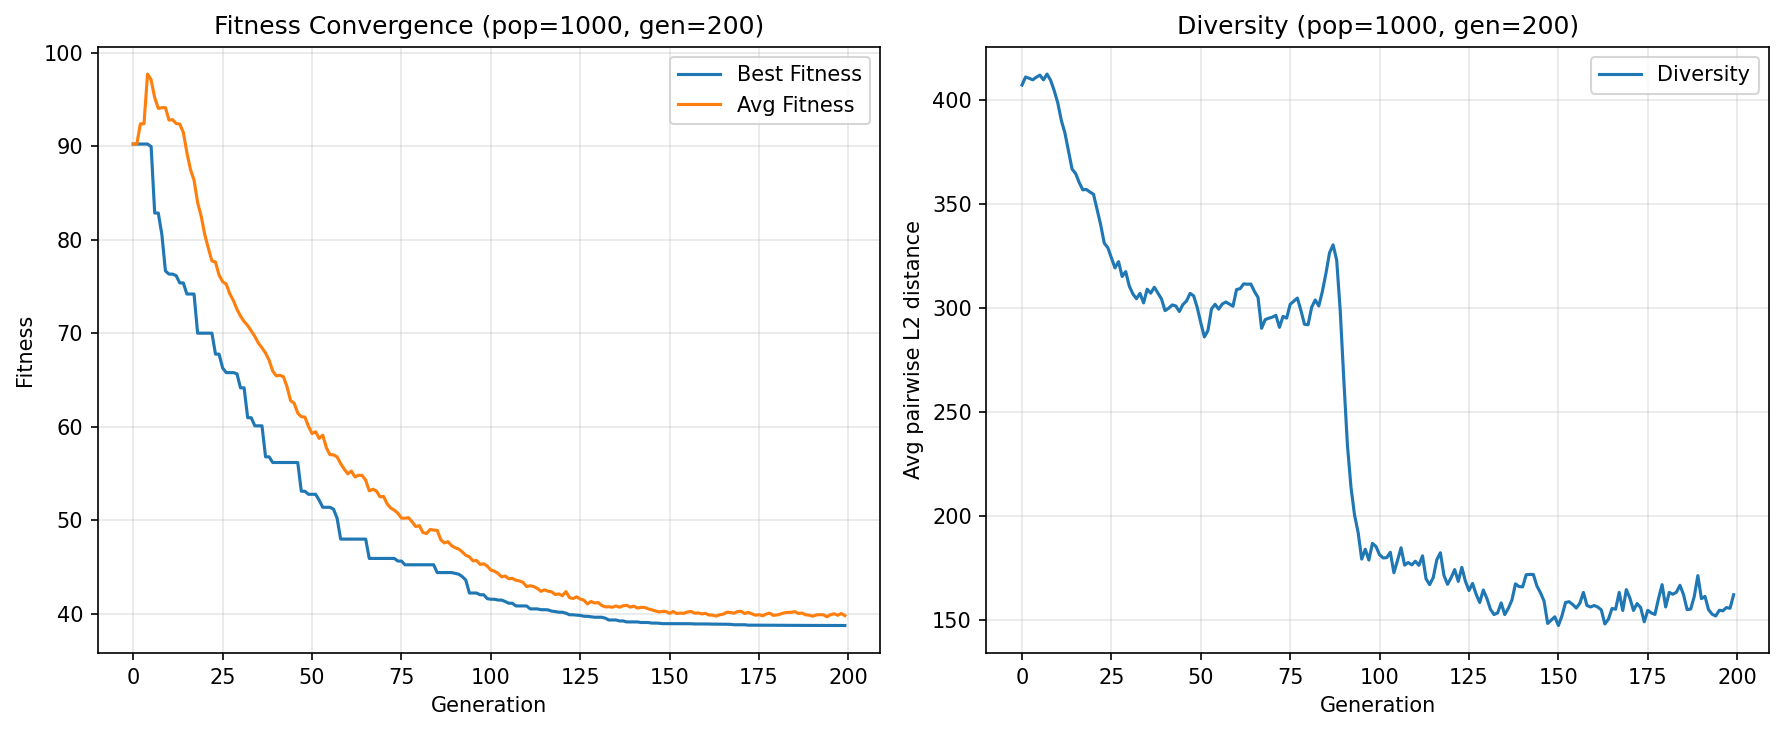
\includegraphics[width=0.9\linewidth]{ga_grid_results_incremental/pop_1000/pop_1000_gen_200.png}
    \caption{Fitness convergence and diversity plot for population size 1000 and 200 generations.}
\end{figure}

\begin{figure}[H]
    \centering
    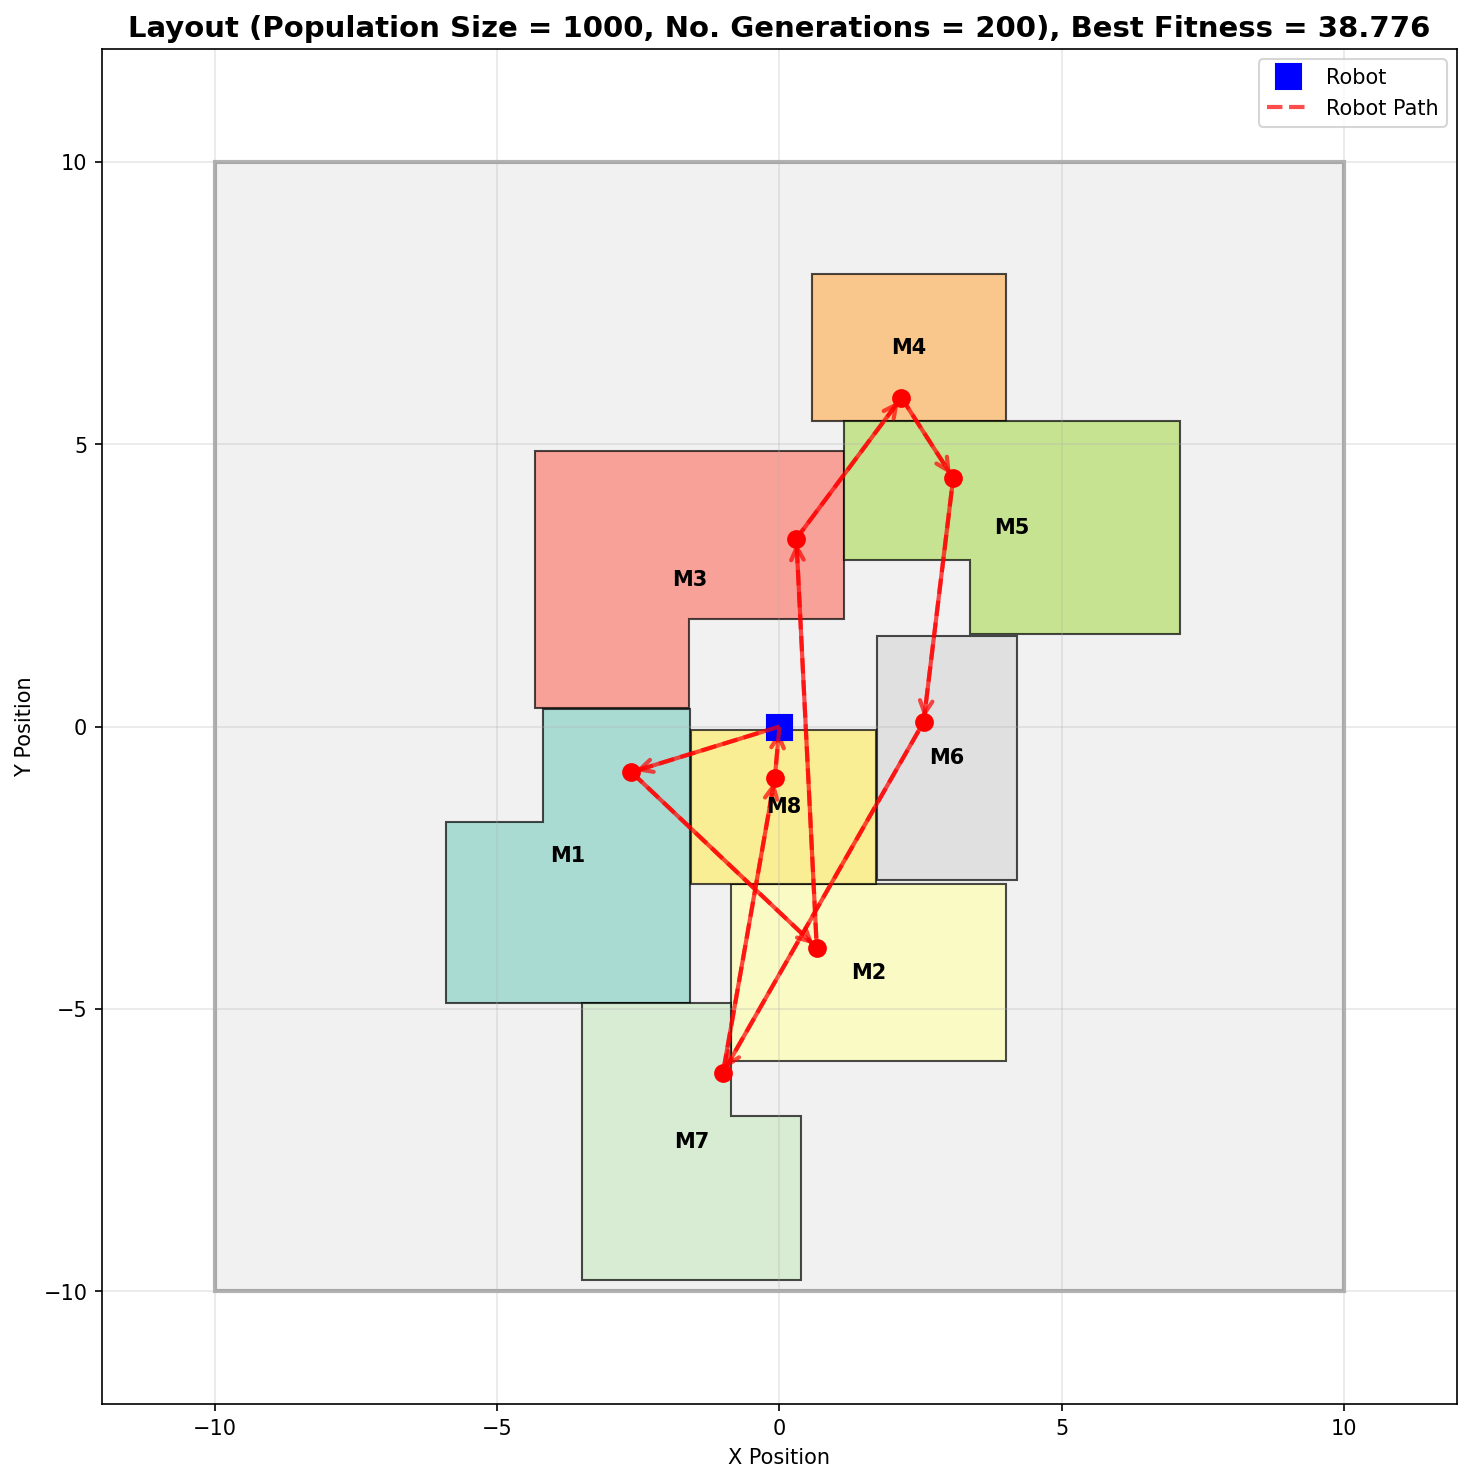
\includegraphics[width=0.7\linewidth]{ga_grid_results_incremental/pop_1000/layout_pop_1000_gen_200.png}
    \caption{Final optimized layout for population size 1000 and 200 generations.}
\end{figure}

\clearpage

\subsubsection{Generations = 500}
\begin{figure}[H]
    \centering
    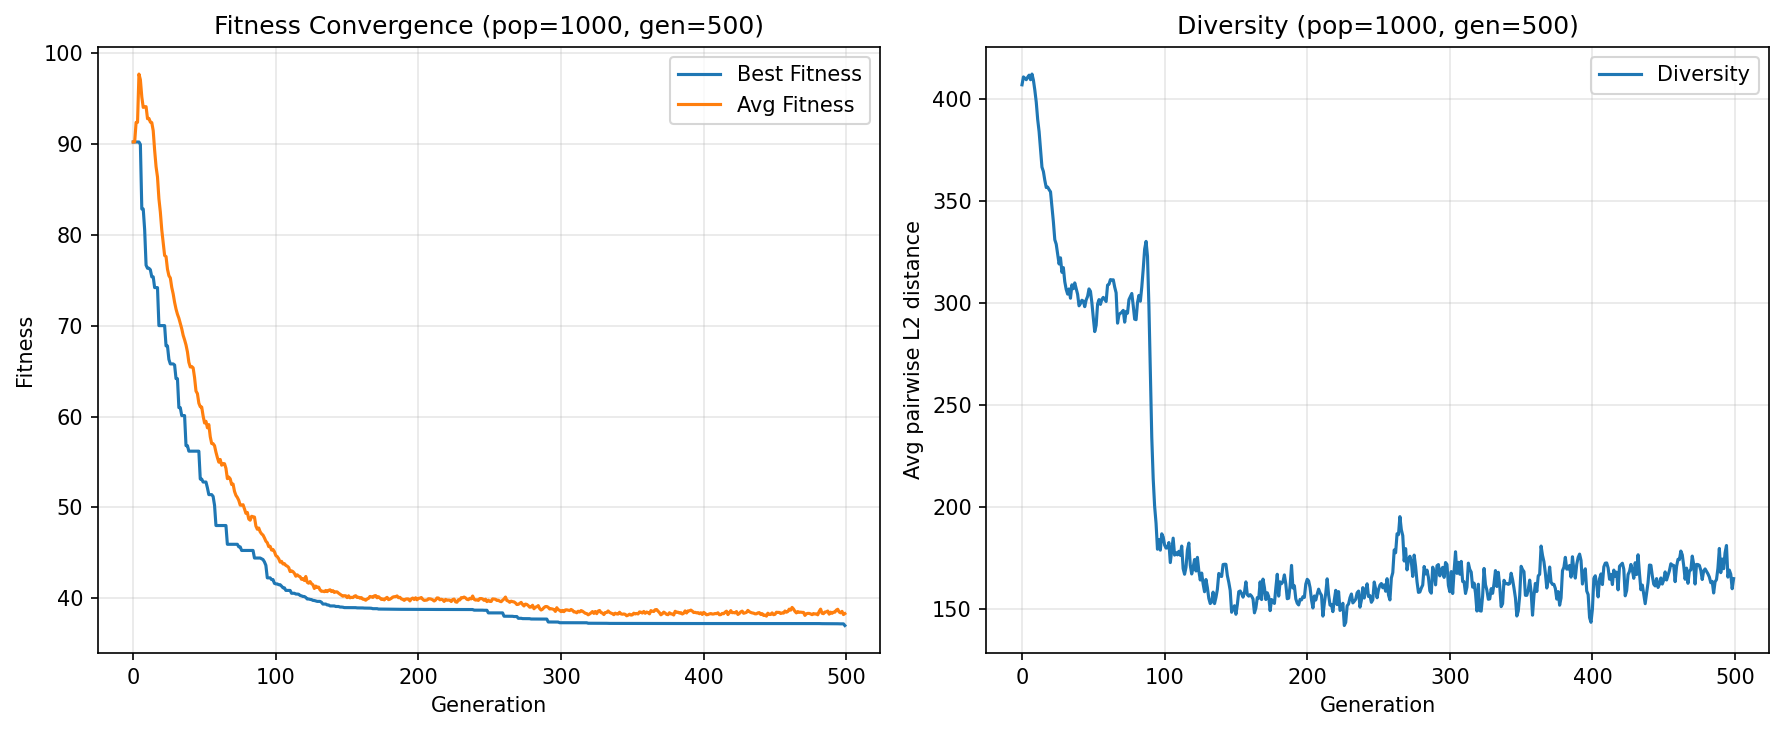
\includegraphics[width=0.9\linewidth]{ga_grid_results_incremental/pop_1000/pop_1000_gen_500.png}
    \caption{Fitness convergence and diversity plot for population size 1000 and 500 generations.}
\end{figure}

\begin{figure}[H]
    \centering
    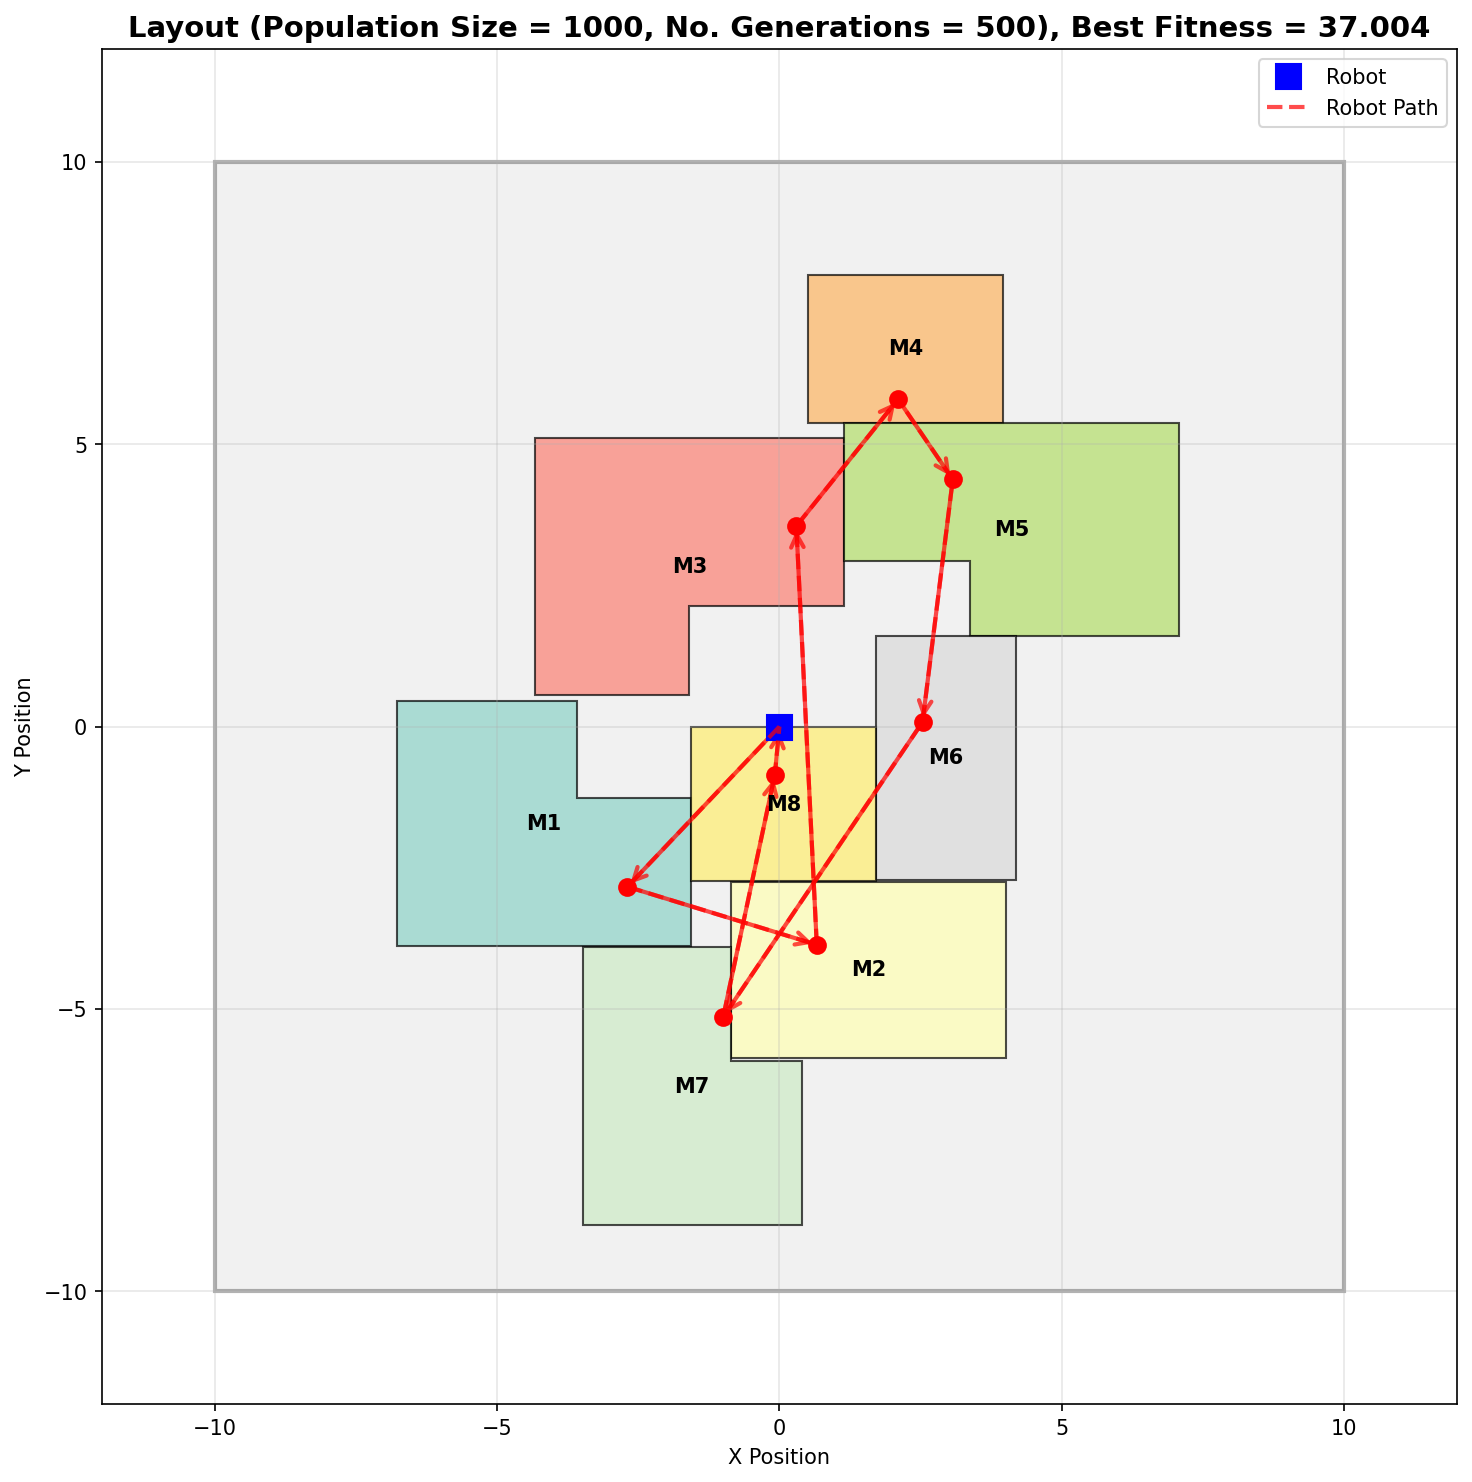
\includegraphics[width=0.7\linewidth]{ga_grid_results_incremental/pop_1000/layout_pop_1000_gen_500.png}
    \caption{Final optimized layout for population size 1000 and 500 generations.}
\end{figure}

\clearpage

\subsubsection{Generations = 1000}
\begin{figure}[H]
    \centering
    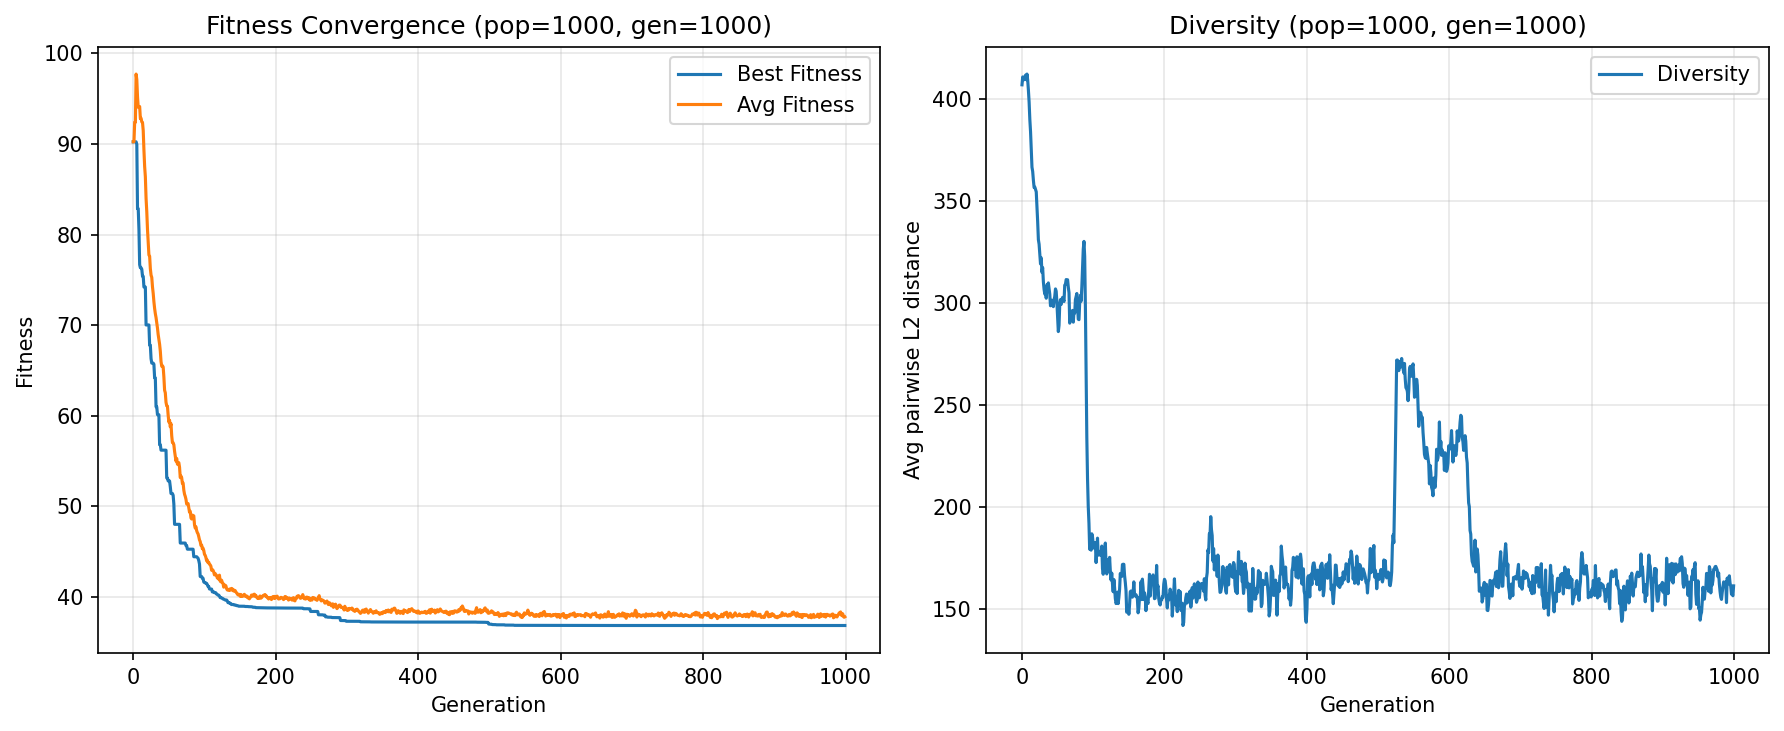
\includegraphics[width=0.9\linewidth]{ga_grid_results_incremental/pop_1000/pop_1000_gen_1000.png}
    \caption{Fitness convergence and diversity plot for population size 1000 and 1000 generations.}
\end{figure}

\begin{figure}[H]
    \centering
    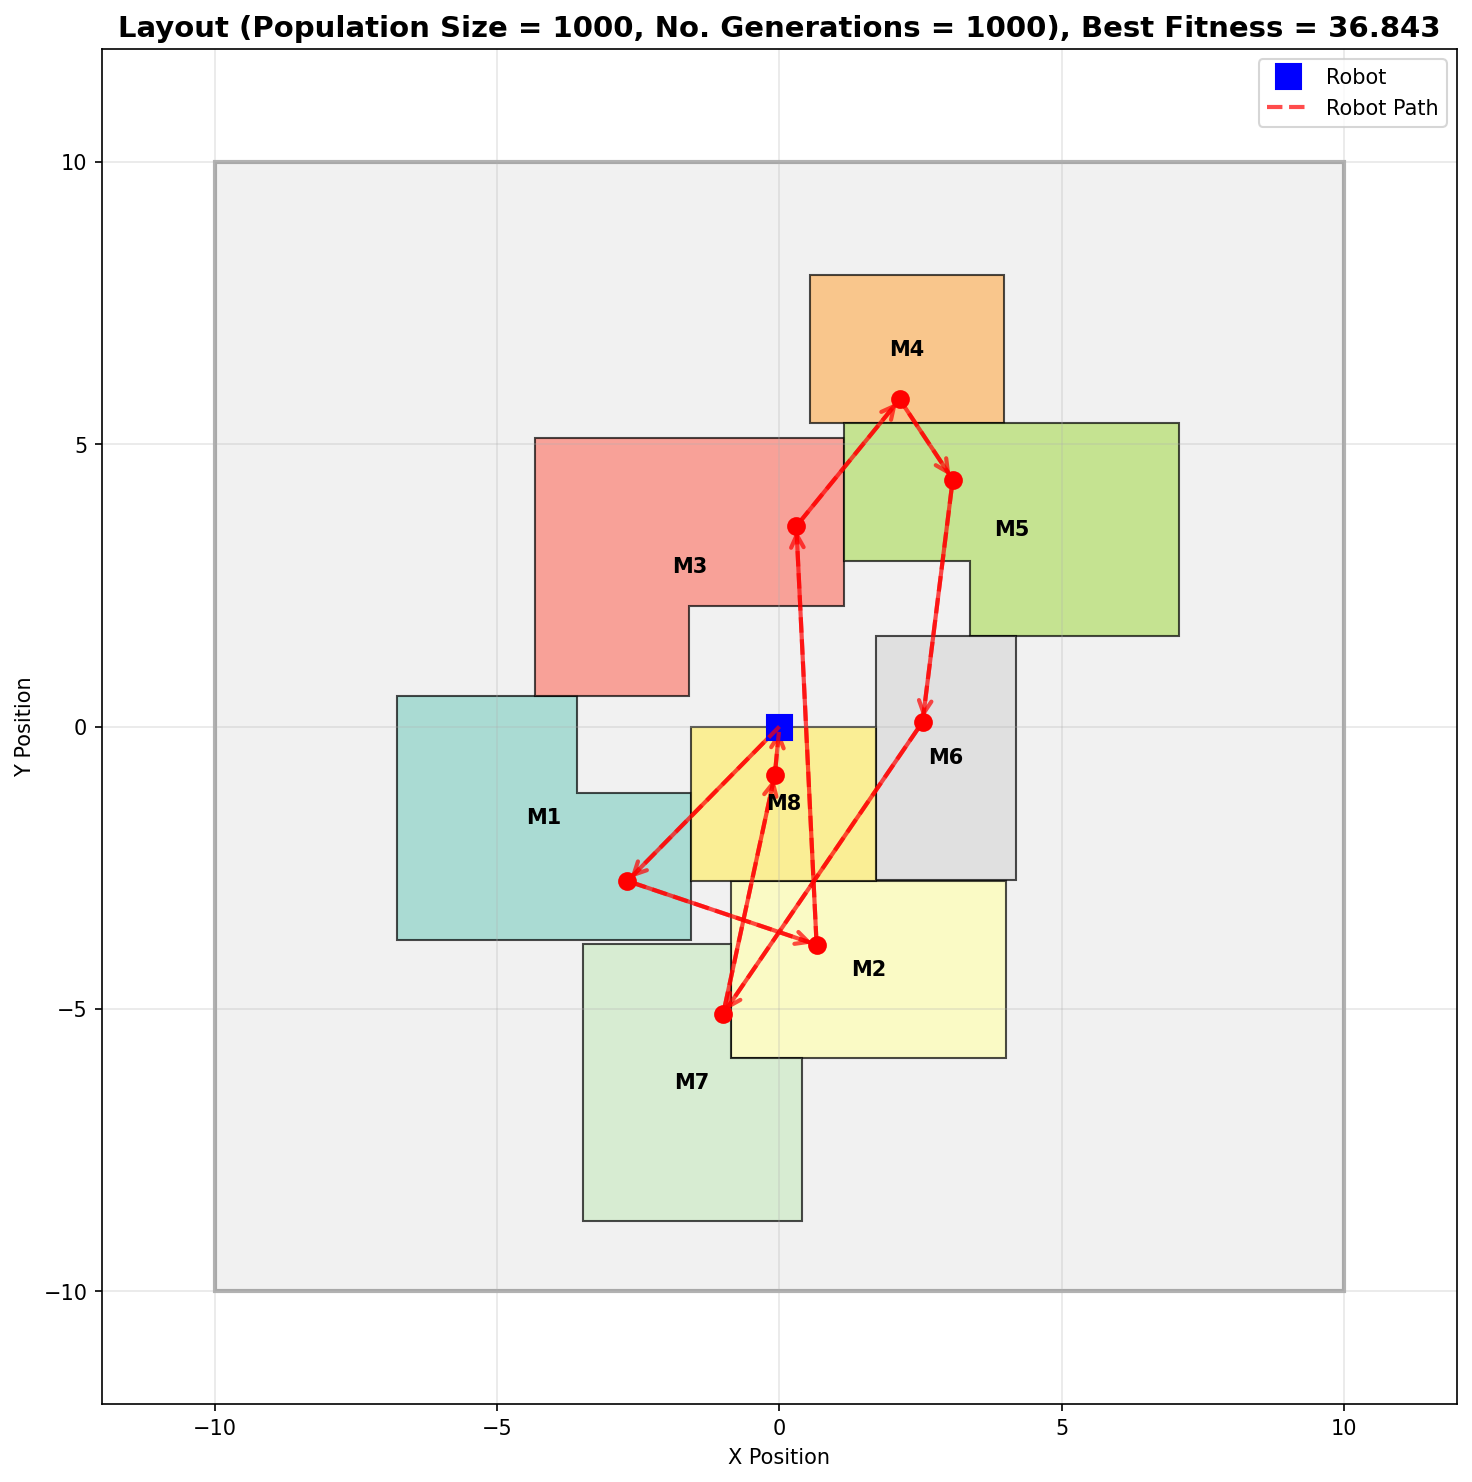
\includegraphics[width=0.7\linewidth]{ga_grid_results_incremental/pop_1000/layout_pop_1000_gen_1000.png}
    \caption{Final optimized layout for population size 1000 and 1000 generations.}
\end{figure}

\clearpage

\subsubsection{Generations = 2000}
\begin{figure}[H]
    \centering
    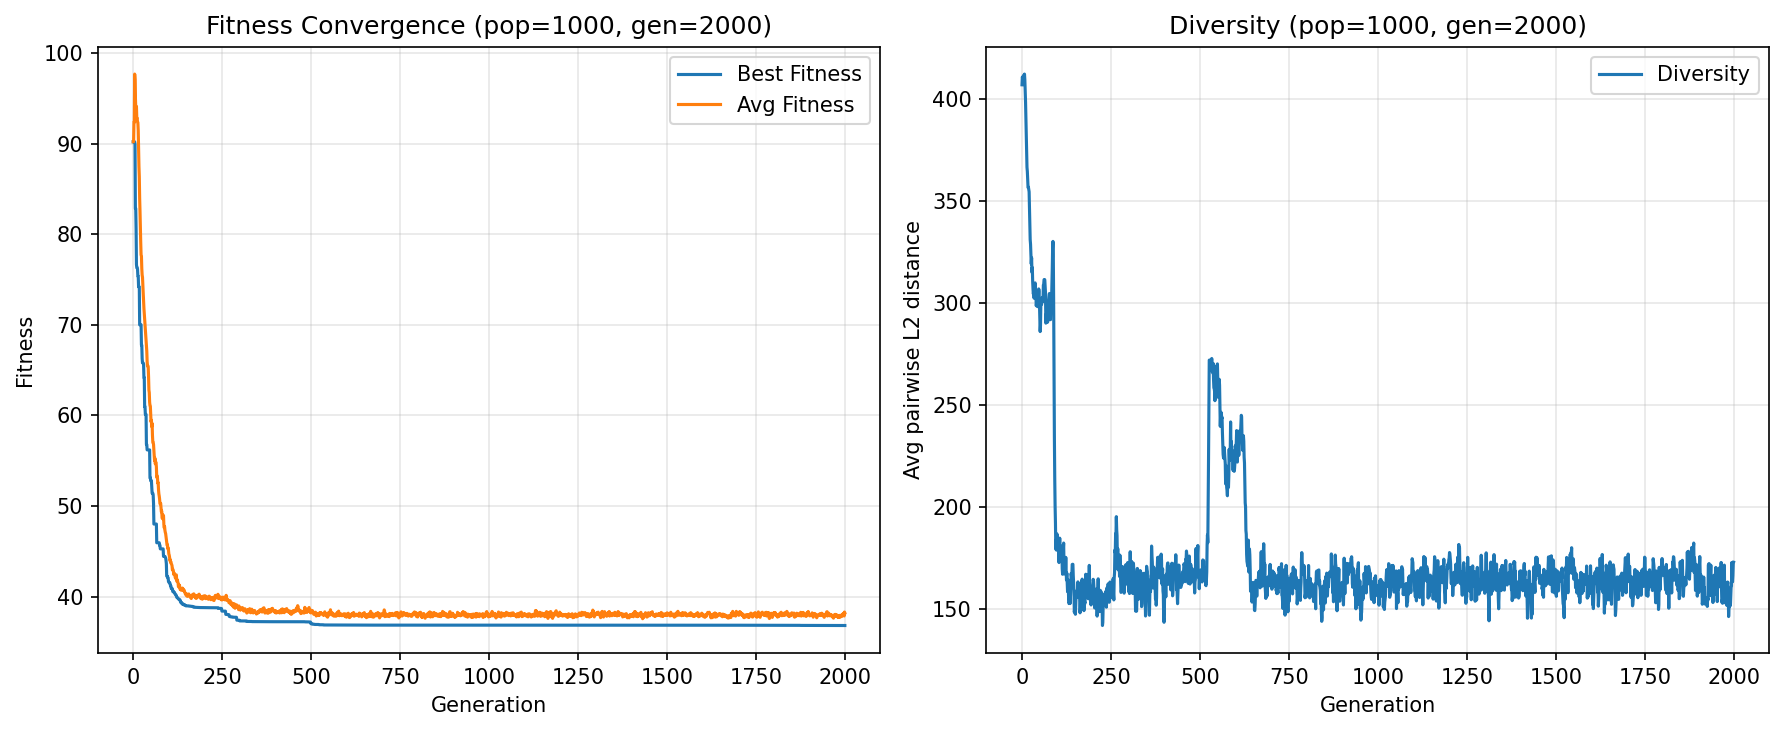
\includegraphics[width=0.9\linewidth]{ga_grid_results_incremental/pop_1000/pop_1000_gen_2000.png}
    \caption{Fitness convergence and diversity plot for population size 1000 and 2000 generations.}
\end{figure}

\begin{figure}[H]
    \centering
    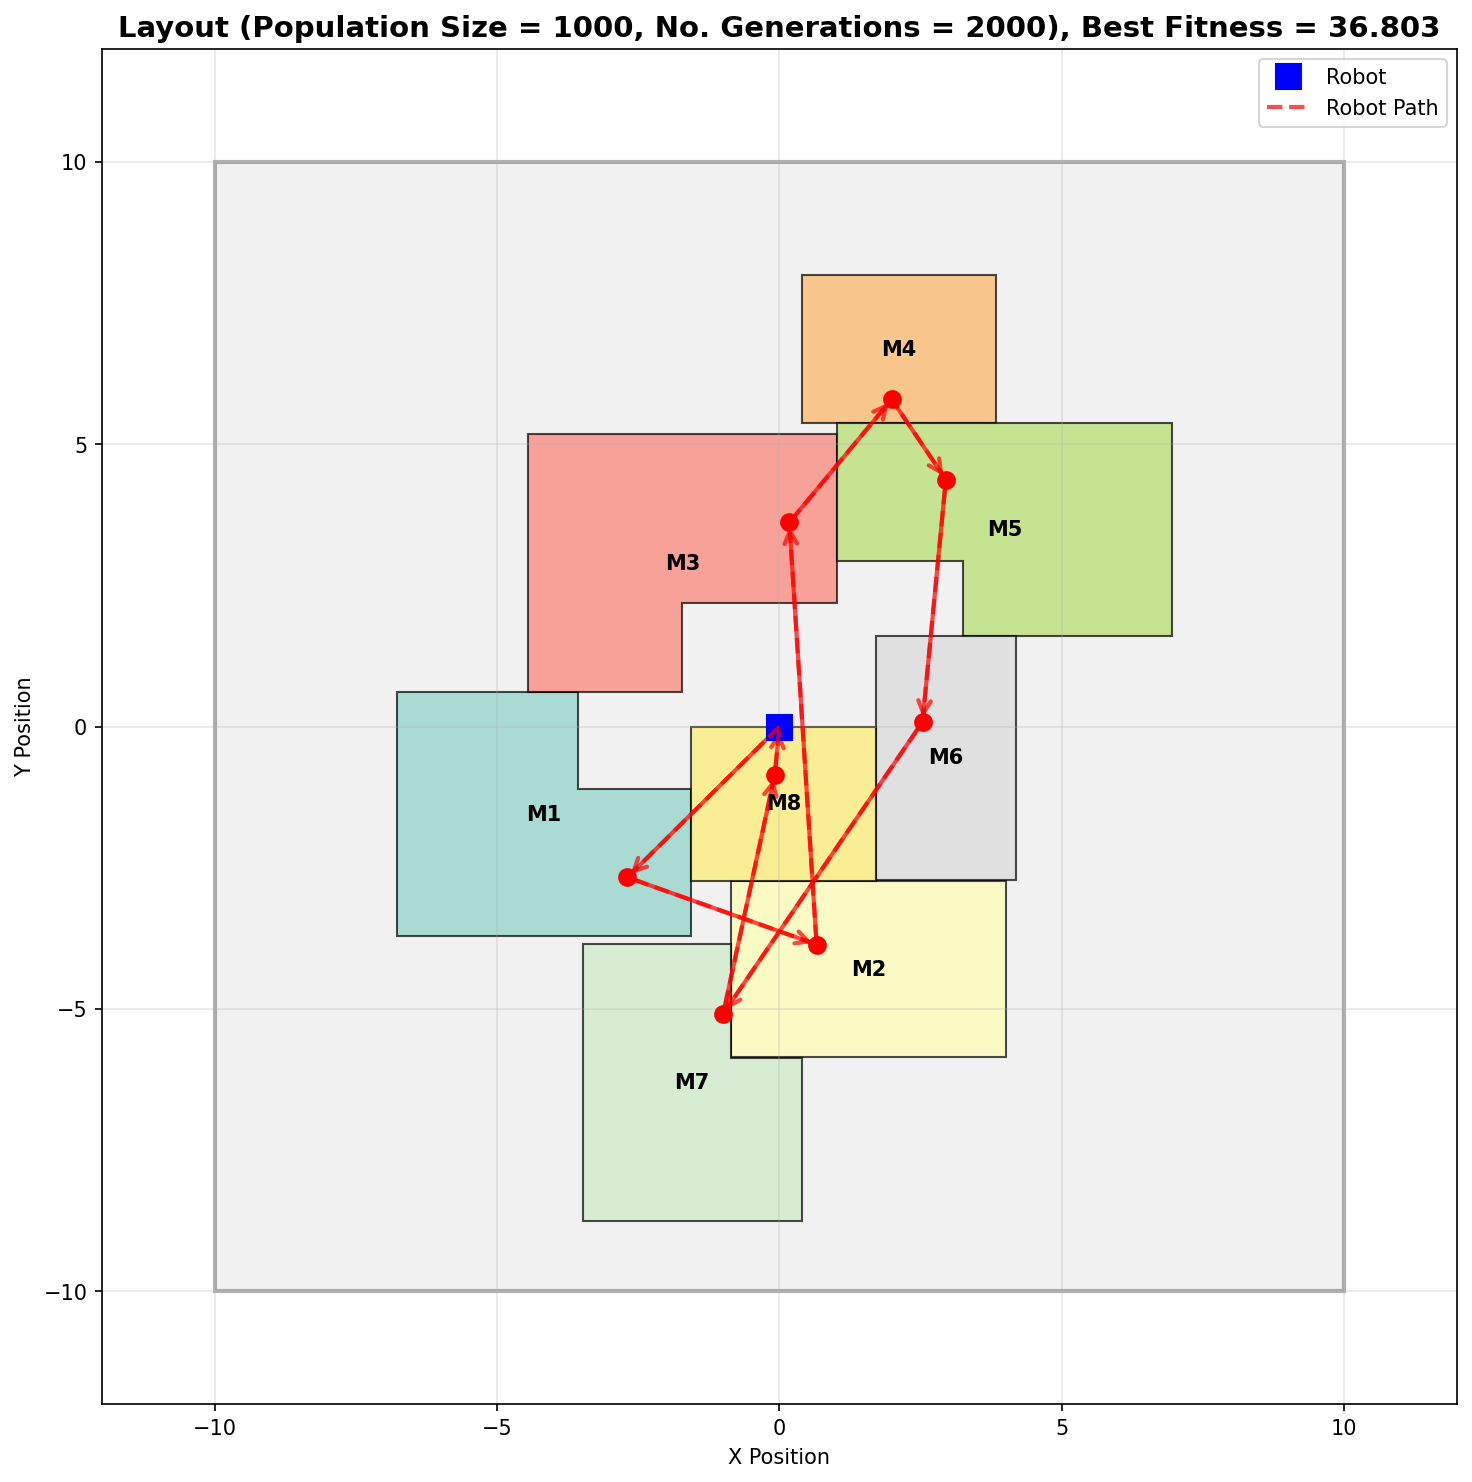
\includegraphics[width=0.7\linewidth]{ga_grid_results_incremental/pop_1000/layout_pop_1000_gen_2000.png}
    \caption{Final optimized layout for population size 1000 and 2000 generations.}
\end{figure}

\clearpage

%====================================================
\subsection{Population Size = 2000}
%====================================================

\subsubsection{Generations = 100}
\begin{figure}[H]
    \centering
    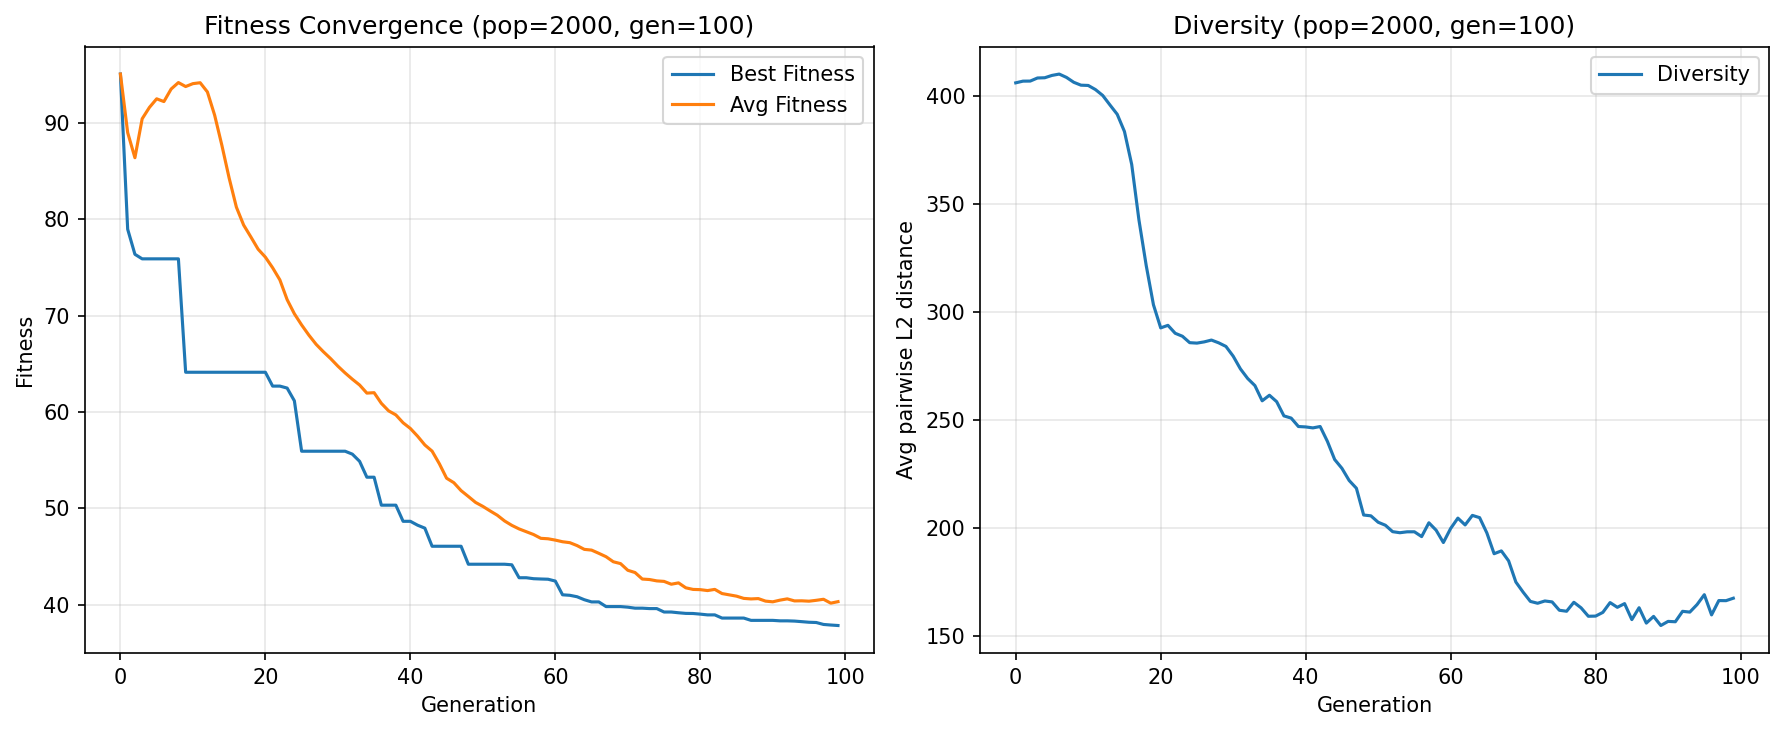
\includegraphics[width=0.9\linewidth]{ga_grid_results_incremental/pop_2000/pop_2000_gen_100.png}
    \caption{Fitness convergence and diversity plot for population size 2000 and 100 generations.}
\end{figure}

\begin{figure}[H]
    \centering
    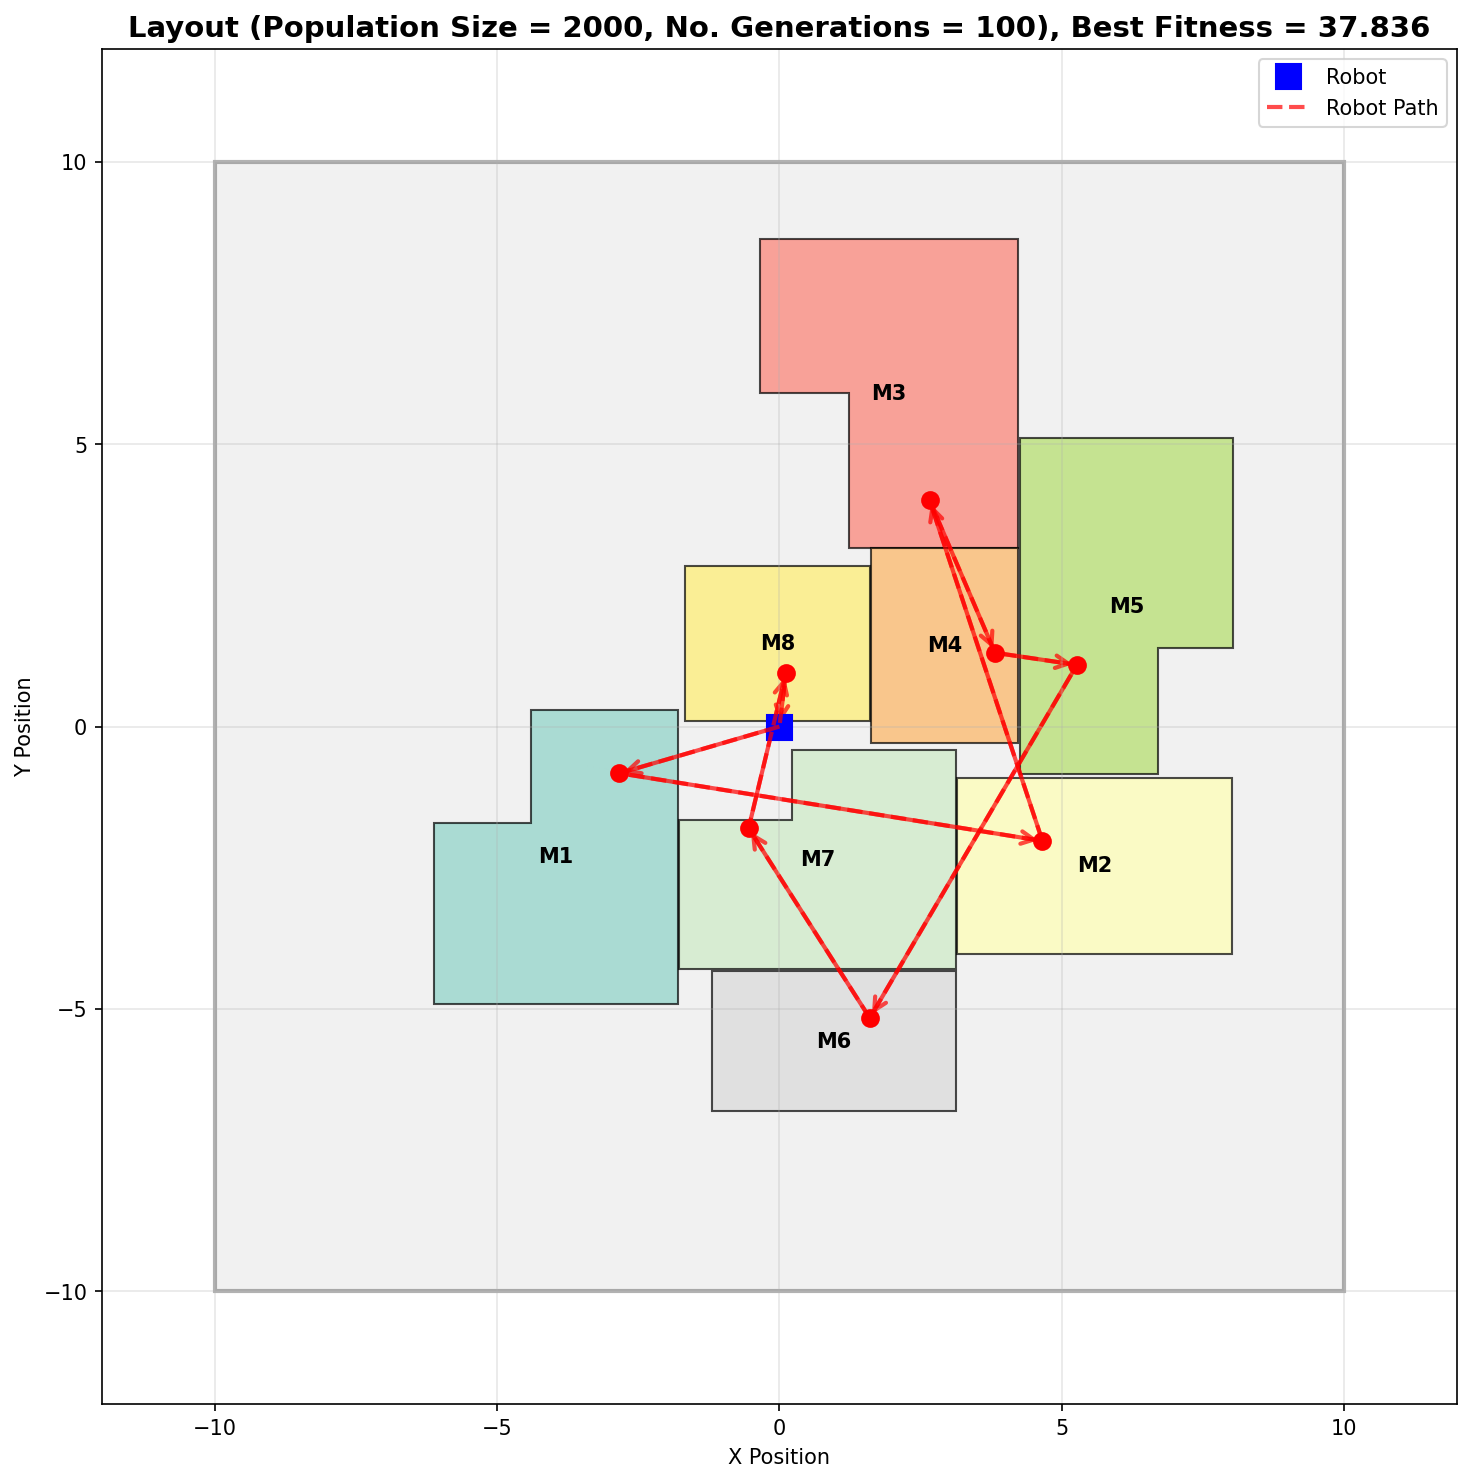
\includegraphics[width=0.7\linewidth]{ga_grid_results_incremental/pop_2000/layout_pop_2000_gen_100.png}
    \caption{Final optimized layout for population size 2000 and 100 generations.}
\end{figure}

\clearpage

\subsubsection{Generations = 200}
\begin{figure}[H]
    \centering
    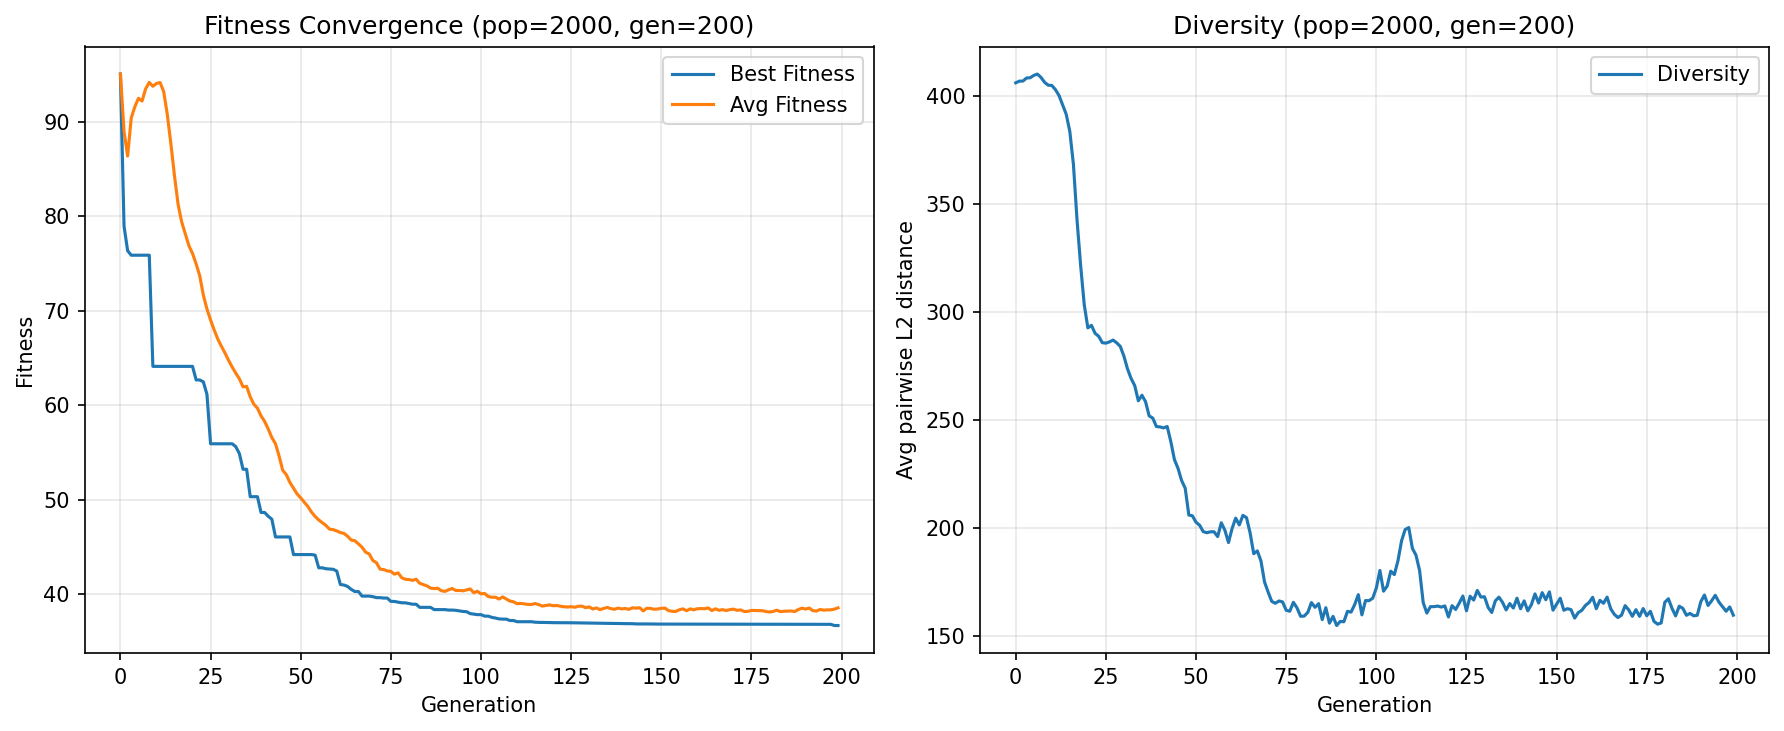
\includegraphics[width=0.9\linewidth]{ga_grid_results_incremental/pop_2000/pop_2000_gen_200.png}
    \caption{Fitness convergence and diversity plot for population size 2000 and 200 generations.}
\end{figure}

\begin{figure}[H]
    \centering
    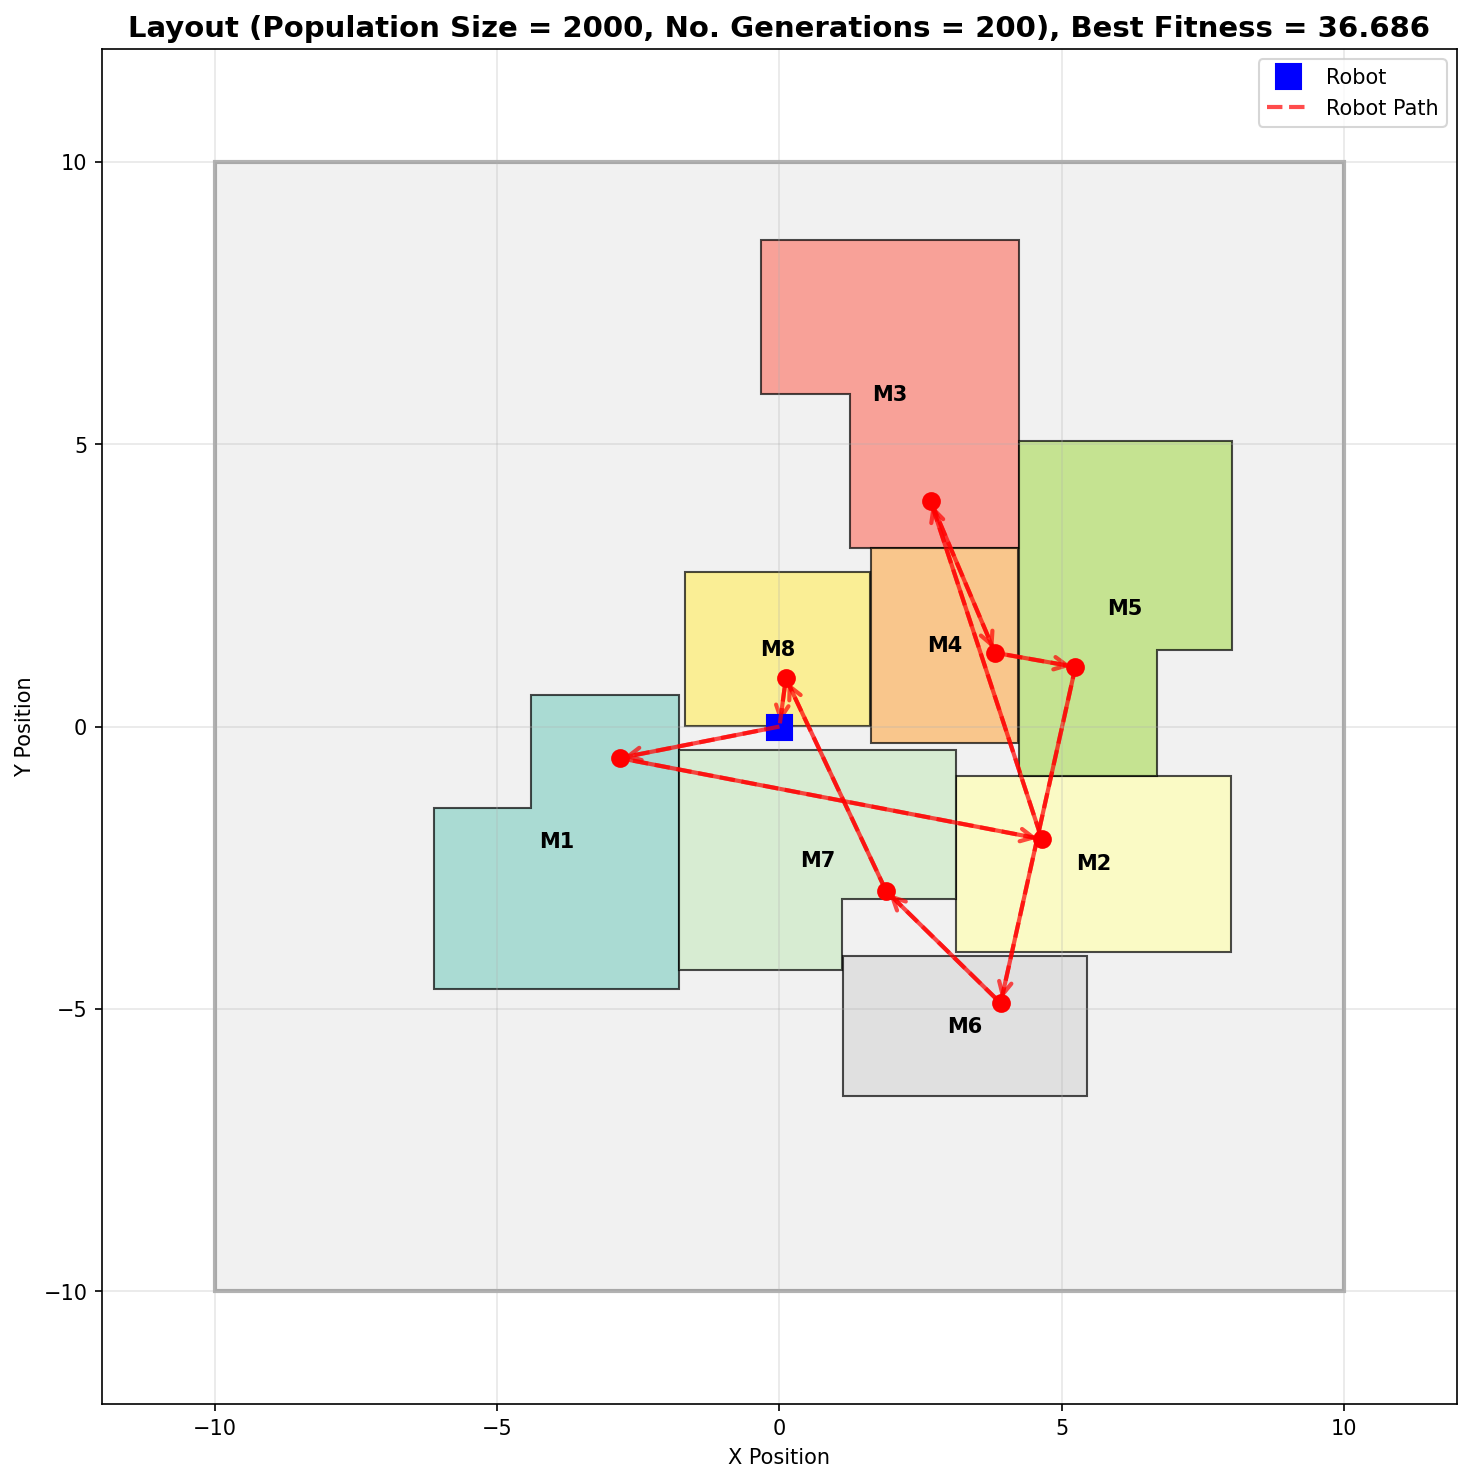
\includegraphics[width=0.7\linewidth]{ga_grid_results_incremental/pop_2000/layout_pop_2000_gen_200.png}
    \caption{Final optimized layout for population size 2000 and 200 generations.}
\end{figure}

\clearpage

\subsubsection{Generations = 500}
\begin{figure}[H]
    \centering
    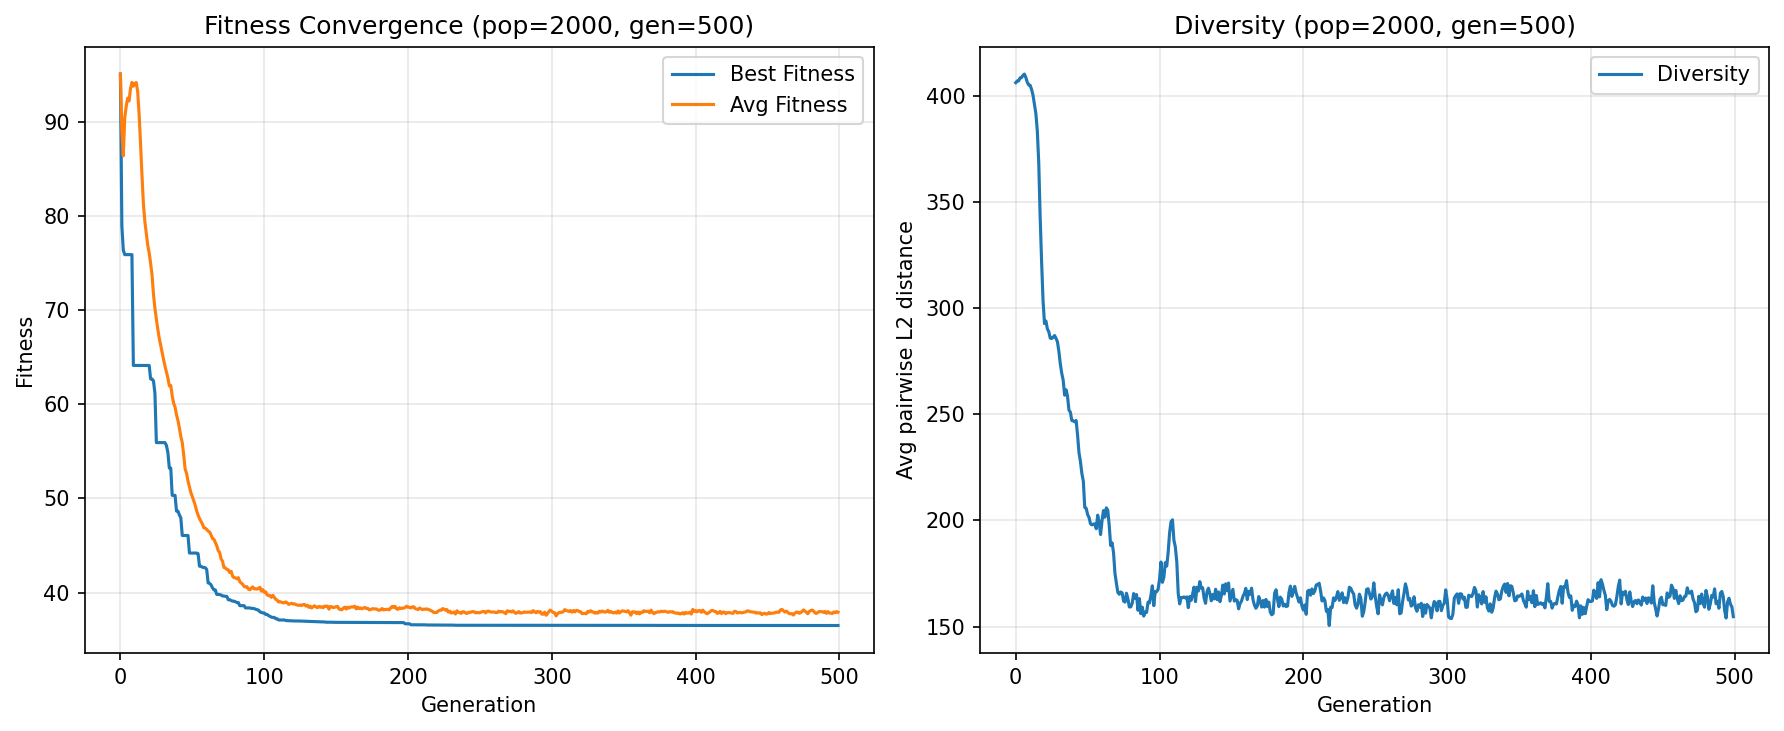
\includegraphics[width=0.9\linewidth]{ga_grid_results_incremental/pop_2000/pop_2000_gen_500.png}
    \caption{Fitness convergence and diversity plot for population size 2000 and 500 generations.}
\end{figure}

\begin{figure}[H]
    \centering
    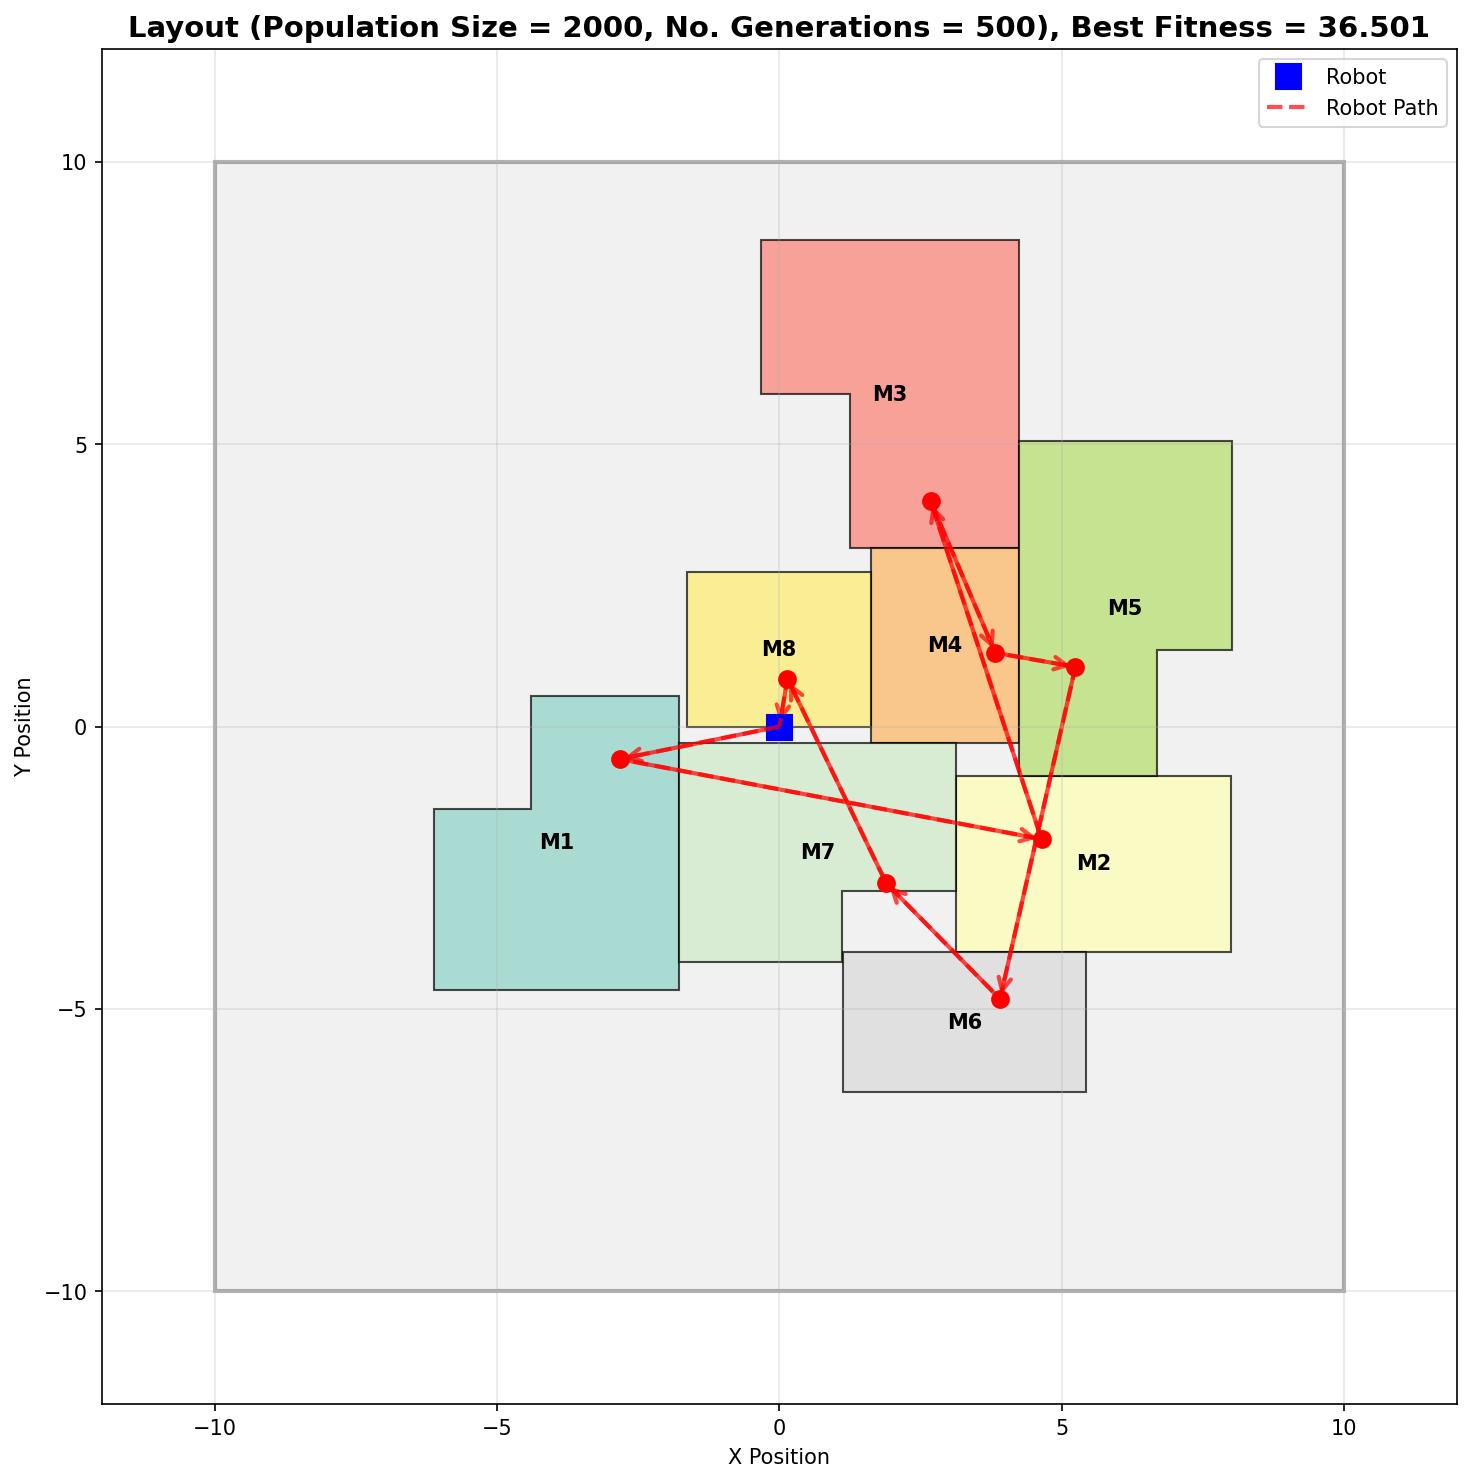
\includegraphics[width=0.7\linewidth]{ga_grid_results_incremental/pop_2000/layout_pop_2000_gen_500.png}
    \caption{Final optimized layout for population size 2000 and 500 generations.}
\end{figure}

\clearpage

\subsubsection{Generations = 1000}
\begin{figure}[H]
    \centering
    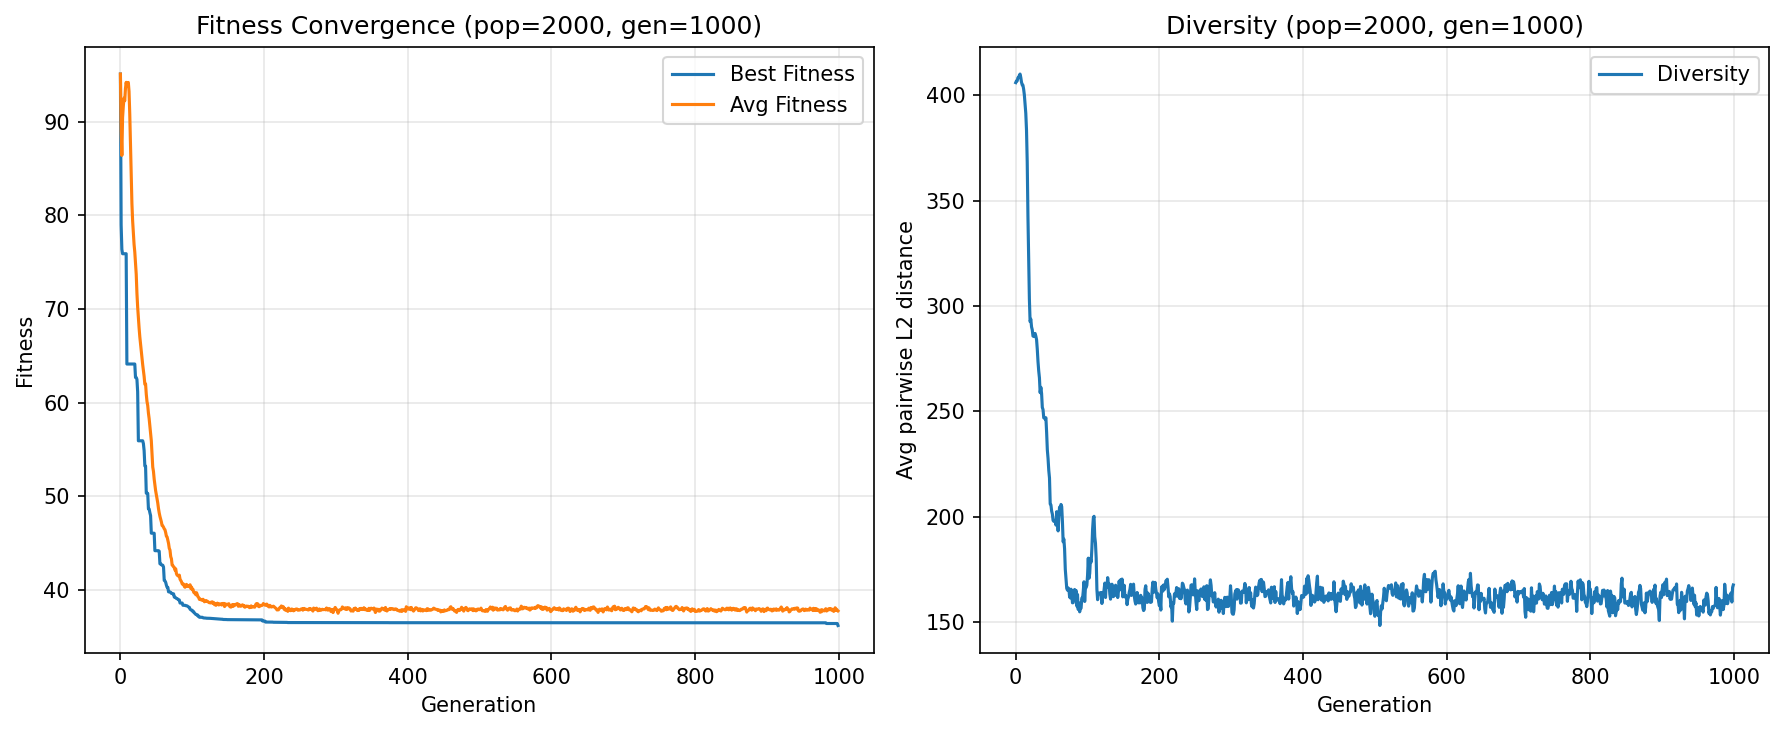
\includegraphics[width=0.9\linewidth]{ga_grid_results_incremental/pop_2000/pop_2000_gen_1000.png}
    \caption{Fitness convergence and diversity plot for population size 2000 and 1000 generations.}
\end{figure}

\begin{figure}[H]
    \centering
    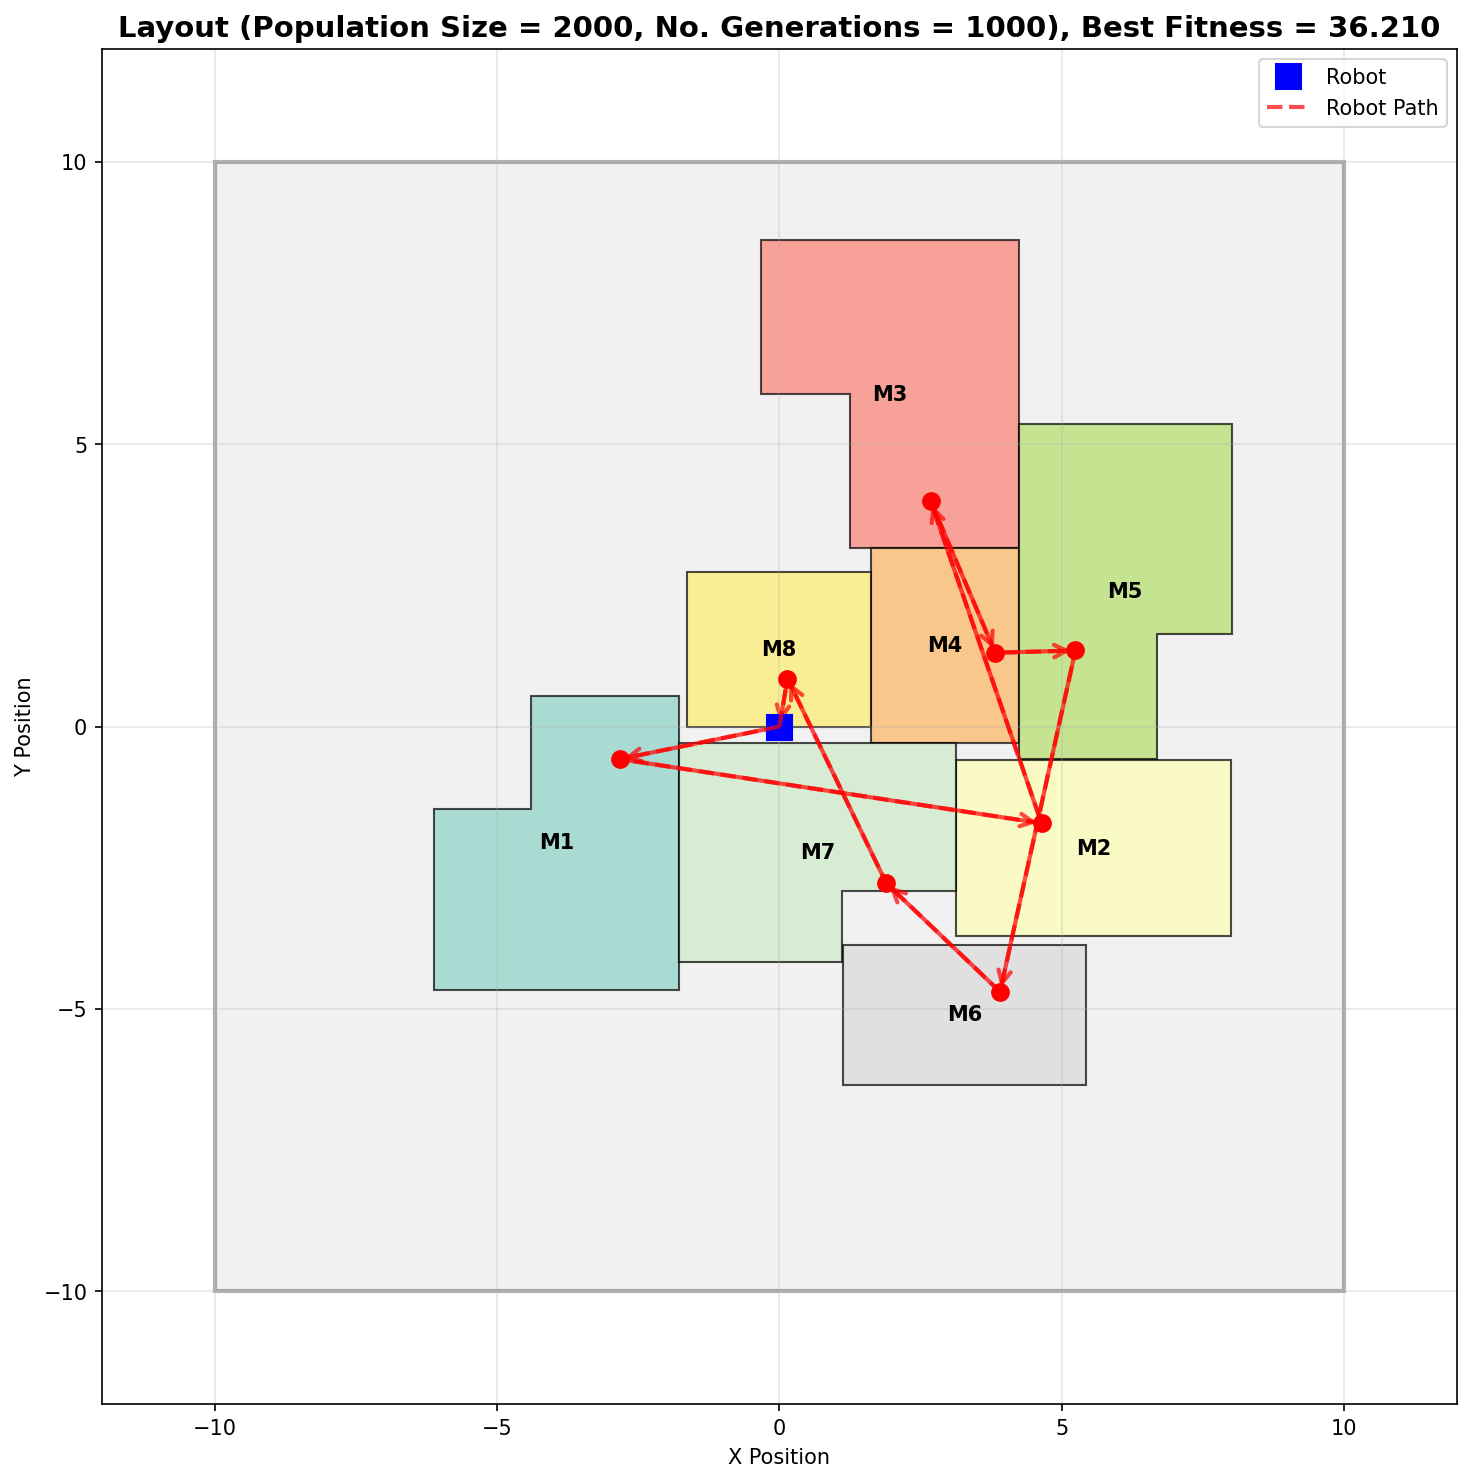
\includegraphics[width=0.7\linewidth]{ga_grid_results_incremental/pop_2000/layout_pop_2000_gen_1000.png}
    \caption{Final optimized layout for population size 2000 and 1000 generations.}
\end{figure}

\clearpage

\subsubsection{Generations = 2000}
\begin{figure}[H]
    \centering
    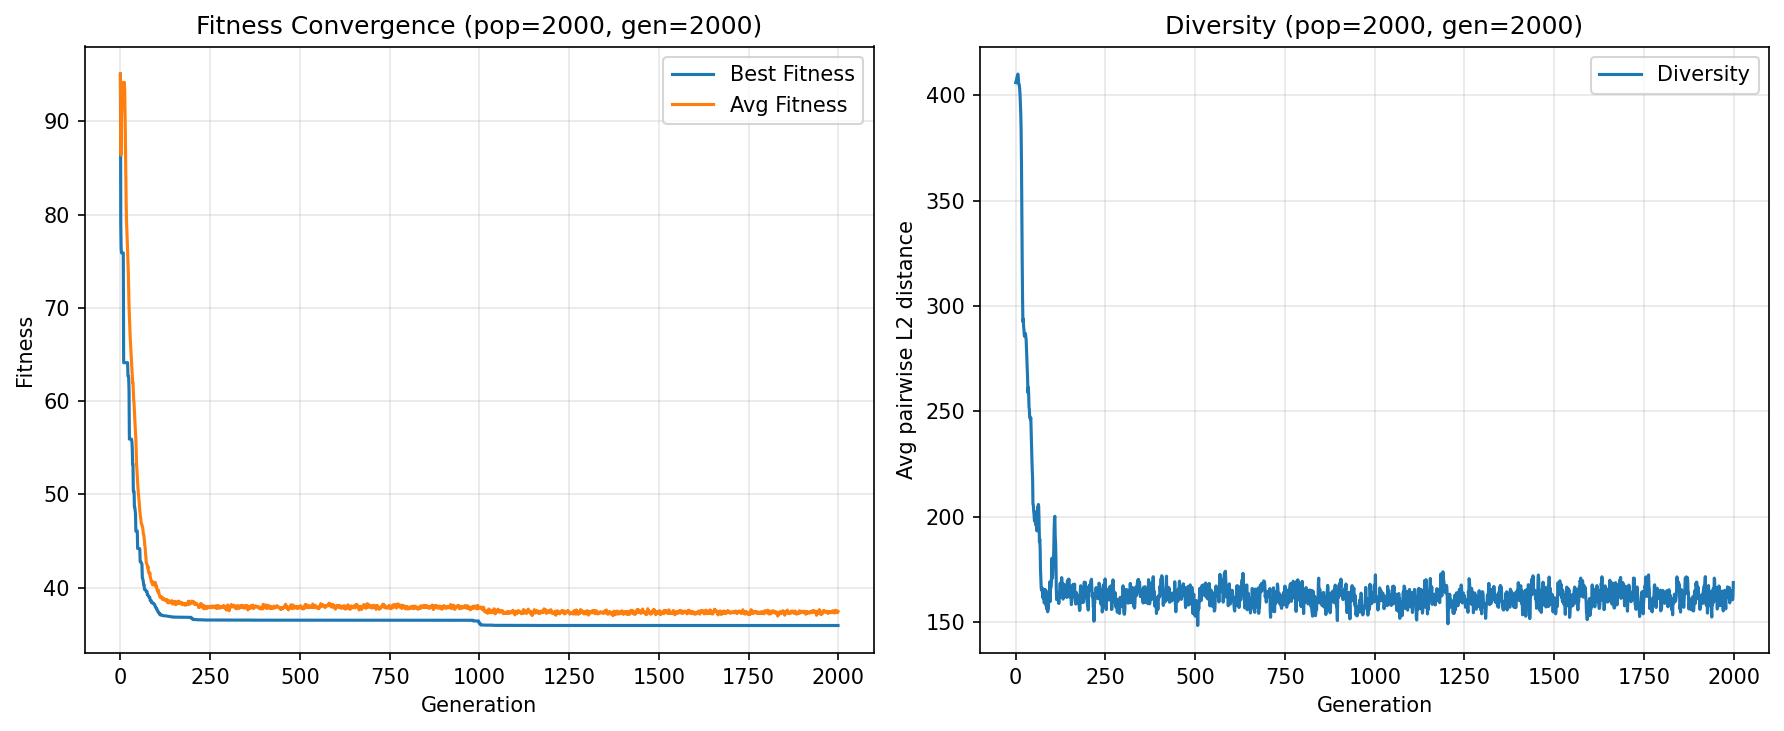
\includegraphics[width=0.9\linewidth]{ga_grid_results_incremental/pop_2000/pop_2000_gen_2000.png}
    \caption{Fitness convergence and diversity plot for population size 2000 and 2000 generations.}
\end{figure}

\begin{figure}[H]
    \centering
    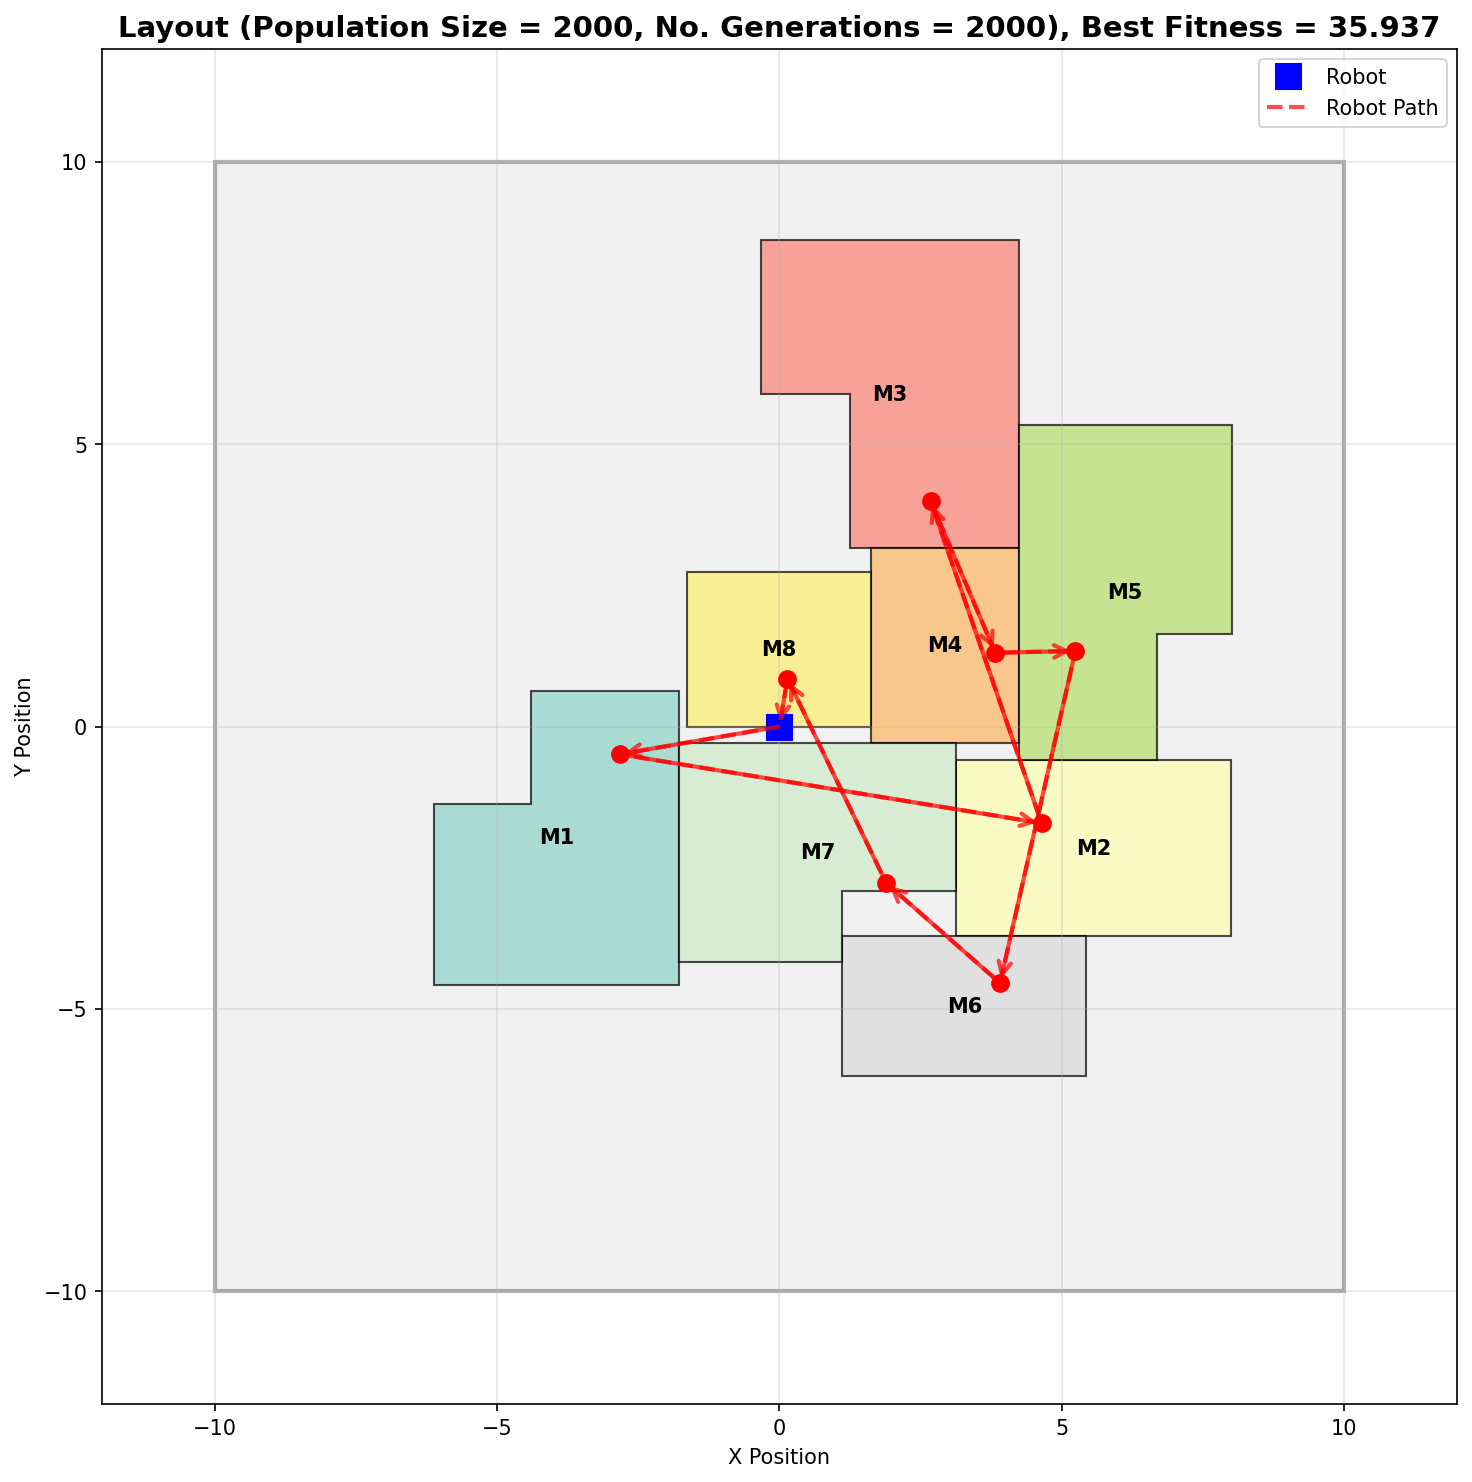
\includegraphics[width=0.7\linewidth]{ga_grid_results_incremental/pop_2000/layout_pop_2000_gen_2000.png}
    \caption{Final optimized layout for population size 2000 and 2000 generations.}
\end{figure}
%====================================================
\section{Appendix: RL Training Machine Definitions}
%====================================================

% ---------- Problem A ----------
\subsection{Problem A}
\begin{table}[H]
\centering
\small
\begin{tabular}{ccccccc}
\toprule
\textbf{ID} & \textbf{Shape} & \textbf{Width} & \textbf{Height} & \textbf{Access Point (x, y)} & \textbf{Cutout Width} & \textbf{Cutout Height} \\
\midrule
M1 & Rectangle & 4.0 & 3.0 & (1.5, 0.0)   & --   & --   \\
M2 & L-shape   & 5.0 & 4.0 & (-1.0, 1.0)  & 2.0  & 2.0  \\
M3 & Rectangle & 3.5 & 2.5 & (0.0, -1.0)  & --   & --   \\
M4 & L-shape   & 4.5 & 3.5 & (1.0, -0.5)  & 1.5  & 1.5  \\
M5 & L-shape   & 3.5 & 5.5 & (1.0, -1.0)  & 1.0  & 2.0  \\
M6 & L-shape   & 3.5 & 5.5 & (1.0, -1.0)  & 1.0  & 2.0  \\
M7 & L-shape   & 3.5 & 5.5 & (1.0, -1.0)  & 1.0  & 2.0  \\
M8 & Rectangle & 3.5 & 2.5 & (0.0, -1.0)  & --   & --   \\
\bottomrule
\end{tabular}
\caption{Machine Configuration for Problem A}
\label{tab:machine_config_a}
\end{table}

% ---------- Problem B ----------
\subsection{Problem B}
\begin{table}[H]
\centering
\small
\begin{tabular}{ccccccc}
\toprule
\textbf{ID} & \textbf{Shape} & \textbf{Width} & \textbf{Height} & \textbf{Access Point (x, y)} & \textbf{Cutout Width} & \textbf{Cutout Height} \\
\midrule
M1 & Rectangle & 4.0 & 3.0 & (1.5, 0.0)   & --   & --   \\
M2 & L-shape   & 5.0 & 4.0 & (-1.0, 1.0)  & 2.0  & 2.0  \\
M3 & Rectangle & 3.5 & 2.5 & (0.0, -1.0)  & --   & --   \\
M4 & L-shape   & 4.5 & 3.5 & (1.0, -0.5)  & 1.5  & 1.5  \\
M5 & L-shape   & 3.0 & 5.5 & (1.0, -1.0)  & 1.0  & 2.0  \\
M6 & L-shape   & 5.0 & 3.0 & (1.0, -1.0)  & 2.0  & 2.0  \\
M7 & L-shape   & 3.5 & 2.5 & (1.0, -1.0)  & 1.0  & 2.0  \\
M8 & Rectangle & 3.5 & 2.5 & (0.0, 0.0)   & --   & --   \\
\bottomrule
\end{tabular}
\caption{Machine Configuration for Problem B}
\label{tab:machine_config_b}
\end{table}

% ---------- Problem C ----------
\subsection{Problem C}
\begin{table}[H]
\centering
\small
\begin{tabular}{ccccccc}
\toprule
\textbf{ID} & \textbf{Shape} & \textbf{Width} & \textbf{Height} & \textbf{Access Point (x, y)} & \textbf{Cutout Width} & \textbf{Cutout Height} \\
\midrule
M1 & Rectangle & 6.0 & 3.0 & (2.0, 0.0)   & -- & -- \\
M2 & Rectangle & 5.5 & 2.5 & (-1.0, 0.0)  & -- & -- \\
M3 & Rectangle & 4.5 & 3.0 & (0.0, -1.0)  & -- & -- \\
M4 & Rectangle & 3.5 & 4.0 & (0.0, 1.5)   & -- & -- \\
M5 & Rectangle & 4.0 & 4.0 & (1.0, -1.0)  & -- & -- \\
M6 & Rectangle & 5.0 & 3.5 & (-1.5, 0.0)  & -- & -- \\
M7 & Rectangle & 6.0 & 2.5 & (0.0, 1.0)   & -- & -- \\
M8 & Rectangle & 4.0 & 2.0 & (0.5, 0.0)   & -- & -- \\
\bottomrule
\end{tabular}
\caption{Machine Configuration for Problem C}
\label{tab:machine_config_c}
\end{table}

% ---------- Problem D ----------
\subsection{Problem D}
\begin{table}[H]
\centering
\small
\begin{tabular}{ccccccc}
\toprule
\textbf{ID} & \textbf{Shape} & \textbf{Width} & \textbf{Height} & \textbf{Access Point (x, y)} & \textbf{Cutout Width} & \textbf{Cutout Height} \\
\midrule
M1 & Rectangle & 2.5 & 2.5 & (0.5, 0.0)   & --   & --   \\
M2 & L-shape   & 3.0 & 3.0 & (1.0, -0.5)  & 1.0  & 1.0  \\
M3 & Rectangle & 2.0 & 2.0 & (0.0, 1.0)   & --   & --   \\
M4 & L-shape   & 3.5 & 3.5 & (-0.5, 1.0)  & 1.0  & 1.2  \\
M5 & Rectangle & 2.0 & 3.0 & (0.5, -1.0)  & --   & --   \\
M6 & Rectangle & 3.0 & 2.0 & (1.0, 0.0)   & --   & --   \\
M7 & L-shape   & 3.0 & 3.5 & (1.0, 1.0)   & 1.0  & 1.0  \\
M8 & Rectangle & 2.5 & 2.0 & (0.0, 0.0)   & --   & --   \\
\bottomrule
\end{tabular}
\caption{Machine Configuration for Problem D}
\label{tab:machine_config_d}
\end{table}

% ---------- Problem E ----------
\subsection{Problem E}
\begin{table}[H]
\centering
\small
\begin{tabular}{ccccccc}
\toprule
\textbf{ID} & \textbf{Shape} & \textbf{Width} & \textbf{Height} & \textbf{Access Point (x, y)} & \textbf{Cutout Width} & \textbf{Cutout Height} \\
\midrule
M1 & L-shape   & 6.0 & 6.0 & (1.0, -1.0)  & 2.0  & 2.0  \\
M2 & L-shape   & 5.5 & 5.0 & (-1.0, 1.0)  & 2.0  & 2.0  \\
M3 & Rectangle & 6.0 & 4.0 & (0.0, -1.5)  & --   & --   \\
M4 & L-shape   & 6.5 & 5.5 & (1.0, 1.0)   & 2.5  & 2.0  \\
M5 & Rectangle & 5.0 & 5.0 & (1.5, 0.0)   & --   & --   \\
M6 & L-shape   & 5.0 & 4.5 & (0.0, -1.0)  & 1.5  & 1.5  \\
M7 & Rectangle & 5.5 & 4.0 & (-1.0, 0.0)  & --   & --   \\
M8 & Rectangle & 4.5 & 3.5 & (1.0, 0.0)   & --   & --   \\
\bottomrule
\end{tabular}
\caption{Machine Configuration for Problem E}
\label{tab:machine_config_e}
\end{table}

% ---------- Problem F ----------
\subsection{Problem F}
\begin{table}[H]
\centering
\small
\begin{tabular}{ccccccc}
\toprule
\textbf{ID} & \textbf{Shape} & \textbf{Width} & \textbf{Height} & \textbf{Access Point (x, y)} & \textbf{Cutout Width} & \textbf{Cutout Height} \\
\midrule
M1 & Rectangle & 2.0 & 6.0 & (0.8, 0.0)   & --   & --   \\
M2 & Rectangle & 2.5 & 5.5 & (-0.5, 1.0)  & --   & --   \\
M3 & L-shape   & 3.0 & 6.0 & (0.0, -1.0)  & 1.0  & 2.0  \\
M4 & Rectangle & 2.2 & 6.5 & (1.0, 0.0)   & --   & --   \\
M5 & Rectangle & 1.8 & 5.0 & (1.0, -1.0)  & --   & --   \\
M6 & L-shape   & 3.0 & 5.5 & (-1.0, 1.0)  & 1.0  & 1.5  \\
M7 & Rectangle & 2.5 & 6.0 & (0.0, 1.0)   & --   & --   \\
M8 & L-shape   & 3.5 & 5.0 & (0.5, 0.0)   & 1.0  & 2.0  \\
\bottomrule
\end{tabular}
\caption{Machine Configuration for Problem F}
\label{tab:machine_config_f}
\end{table}

% ---------- Problem G ----------
\subsection{Problem G}
\begin{table}[H]
\centering
\small
\begin{tabular}{ccccccc}
\toprule
\textbf{ID} & \textbf{Shape} & \textbf{Width} & \textbf{Height} & \textbf{Access Point (x, y)} & \textbf{Cutout Width} & \textbf{Cutout Height} \\
\midrule
M1 & Rectangle & 4.0 & 2.5 & (1.0, 0.0)   & --   & --   \\
M2 & Rectangle & 5.0 & 3.5 & (-1.0, 0.0)  & --   & --   \\
M3 & L-shape   & 4.0 & 4.0 & (1.0, 1.0)   & 1.5  & 1.0  \\
M4 & Rectangle & 3.0 & 3.0 & (0.0, -1.0)  & --   & --   \\
M5 & L-shape   & 4.5 & 3.0 & (1.0, -1.0)  & 1.0  & 1.5  \\
M6 & Rectangle & 4.0 & 3.0 & (-1.0, 1.0)  & --   & --   \\
M7 & Rectangle & 3.0 & 2.0 & (0.5, 0.0)   & --   & --   \\
M8 & L-shape   & 4.0 & 3.0 & (0.0, -1.0)  & 1.0  & 1.0  \\
\bottomrule
\end{tabular}
\caption{Machine Configuration for Problem G}
\label{tab:machine_config_g}
\end{table}

% ---------- Problem H ----------
\subsection{Problem H}
\begin{table}[H]
\centering
\small
\begin{tabular}{ccccccc}
\toprule
\textbf{ID} & \textbf{Shape} & \textbf{Width} & \textbf{Height} & \textbf{Access Point (x, y)} & \textbf{Cutout Width} & \textbf{Cutout Height} \\
\midrule
M1 & Rectangle & 3.5 & 4.0 & (1.0, 0.0)   & --   & --   \\
M2 & L-shape   & 4.5 & 4.0 & (0.0, 1.0)   & 1.5  & 1.5  \\
M3 & Rectangle & 5.0 & 3.0 & (-1.0, 0.0)  & --   & --   \\
M4 & L-shape   & 5.0 & 5.0 & (0.0, -1.0)  & 2.0  & 1.5  \\
M5 & Rectangle & 3.0 & 3.5 & (1.0, 1.0)   & --   & --   \\
M6 & Rectangle & 4.0 & 3.0 & (-1.0, -1.0) & --   & --   \\
M7 & L-shape   & 4.5 & 3.5 & (1.0, 0.0)   & 1.5  & 1.0  \\
M8 & Rectangle & 3.5 & 2.0 & (0.0, -0.5)  & --   & --   \\
\bottomrule
\end{tabular}
\caption{Machine Configuration for Problem H}
\label{tab:machine_config_h}
\end{table}

\newpage
\section{Appendix: 10 Problems}
% ---------- Problem 1 ----------
\subsection{Problem 1}
\begin{table}[H]
\centering
\small
\begin{tabular}{ccccccc}
\toprule
\textbf{ID} & \textbf{Shape} & \textbf{Width} & \textbf{Height} & \textbf{Access Point (x, y)} & \textbf{Cutout Width} & \textbf{Cutout Height} \\
\midrule
M1 & L-shape   & 5.332 & 4.175 & (-1.203, -0.441) & 1.780 & 1.581 \\
M2 & Rectangle & 5.935 & 2.826 & (0.514, -0.407)  & --    & --    \\
M3 & L-shape   & 4.467 & 3.008 & (0.499, -0.817)  & 1.565 & 1.021 \\
M4 & Rectangle & 5.923 & 3.719 & (-0.115, 0.642)  & --    & --    \\
M5 & L-shape   & 4.247 & 4.720 & (-1.430, 1.001)  & 1.526 & 2.104 \\
M6 & Rectangle & 5.837 & 4.958 & (-0.971, 0.596)  & --    & --    \\
M7 & L-shape   & 3.327 & 2.901 & (-1.221, -0.558) & 1.011 & 1.385 \\
M8 & Rectangle & 3.873 & 4.450 & (0.144, -0.917)  & --    & --    \\
\bottomrule
\end{tabular}
\caption{Machine configurations for Problem 1.}
\end{table}

% ---------- Problem 2 ----------
\subsection{Problem 2}
\begin{table}[H]
\centering
\small
\begin{tabular}{ccccccc}
\toprule
\textbf{ID} & \textbf{Shape} & \textbf{Width} & \textbf{Height} & \textbf{Access Point (x, y)} & \textbf{Cutout Width} & \textbf{Cutout Height} \\
\midrule
M1 & L-shape   & 5.390 & 2.647 & (0.781, 1.088)   & 1.155 & 1.292 \\
M2 & Rectangle & 5.358 & 3.517 & (-0.377, 0.447)  & --    & --    \\
M3 & L-shape   & 4.203 & 3.930 & (0.323, -1.348)  & 1.812 & 1.684 \\
M4 & Rectangle & 5.767 & 4.287 & (0.467, 0.711)   & --    & --    \\
M5 & L-shape   & 3.563 & 3.755 & (1.185, 1.279)   & 1.015 & 1.770 \\
M6 & Rectangle & 4.909 & 3.517 & (-1.111, 1.088)  & --    & --    \\
M7 & L-shape   & 3.761 & 3.982 & (-1.274, 0.169)  & 1.345 & 1.304 \\
M8 & Rectangle & 3.498 & 2.589 & (1.120, 0.323)   & --    & --    \\
\bottomrule
\end{tabular}
\caption{Machine configurations for Problem 2.}
\end{table}

% ---------- Problem 3 ----------
\subsection{Problem 3}
\begin{table}[H]
\centering
\small
\begin{tabular}{ccccccc}
\toprule
\textbf{ID} & \textbf{Shape} & \textbf{Width} & \textbf{Height} & \textbf{Access Point (x, y)} & \textbf{Cutout Width} & \textbf{Cutout Height} \\
\midrule
M1 & L-shape   & 4.563 & 3.553 & (-0.837, -1.109) & 1.620 & 1.486 \\
M2 & Rectangle & 4.863 & 4.268 & (-0.194, -1.356) & --    & --    \\
M3 & L-shape   & 3.676 & 4.471 & (-0.237, 0.196)  & 1.567 & 1.935 \\
M4 & Rectangle & 3.488 & 3.666 & (0.458, 1.304)   & --    & --    \\
M5 & L-shape   & 3.843 & 4.751 & (1.047, 0.073)   & 1.533 & 2.287 \\
M6 & Rectangle & 4.320 & 3.223 & (0.892, -1.196)  & --    & --    \\
M7 & L-shape   & 5.156 & 4.112 & (-0.326, 1.318)  & 1.961 & 1.164 \\
M8 & Rectangle & 4.250 & 4.886 & (-1.245, 0.931)  & --    & --    \\
\bottomrule
\end{tabular}
\caption{Machine configurations for Problem 3.}
\end{table}

% ---------- Problem 4 ----------
\subsection{Problem 4}
\begin{table}[H]
\centering
\small
\begin{tabular}{ccccccc}
\toprule
\textbf{ID} & \textbf{Shape} & \textbf{Width} & \textbf{Height} & \textbf{Access Point (x, y)} & \textbf{Cutout Width} & \textbf{Cutout Height} \\
\midrule
M1 & L-shape   & 4.492 & 3.400 & (0.666, -0.160)  & 1.565 & 1.018 \\
M2 & Rectangle & 4.005 & 3.689 & (-0.146, -1.236) & --    & --    \\
M3 & L-shape   & 3.885 & 3.347 & (1.206, 0.652)   & 1.847 & 1.022 \\
M4 & Rectangle & 3.685 & 3.845 & (-1.316, -0.812) & --    & --    \\
M5 & L-shape   & 4.679 & 2.502 & (-0.324, -1.406) & 1.322 & 1.225 \\
M6 & Rectangle & 4.160 & 3.170 & (1.234, 1.069)   & --    & --    \\
M7 & L-shape   & 3.765 & 3.568 & (-0.908, 0.793)  & 1.401 & 1.604 \\
M8 & Rectangle & 5.263 & 2.832 & (-1.092, 0.727)  & --    & --    \\
\bottomrule
\end{tabular}
\caption{Machine configurations for Problem 4.}
\end{table}

% ---------- Problem 5 ----------
\subsection{Problem 5}
\begin{table}[H]
\centering
\small
\begin{tabular}{ccccccc}
\toprule
\textbf{ID} & \textbf{Shape} & \textbf{Width} & \textbf{Height} & \textbf{Access Point (x, y)} & \textbf{Cutout Width} & \textbf{Cutout Height} \\
\midrule
M1 & L-shape   & 4.263 & 4.940 & (0.340, 0.579)   & 1.576 & 1.276 \\
M2 & Rectangle & 5.490 & 4.612 & (-0.871, 0.452)  & --    & --    \\
M3 & L-shape   & 5.101 & 4.288 & (0.927, 1.036)   & 1.573 & 1.578 \\
M4 & Rectangle & 5.162 & 2.858 & (-1.420, -1.040) & --    & --    \\
M5 & L-shape   & 5.509 & 3.312 & (-0.591, -1.146) & 1.212 & 1.635 \\
M6 & Rectangle & 3.152 & 4.959 & (0.157, -0.758)  & --    & --    \\
M7 & L-shape   & 3.048 & 4.704 & (-0.331, 1.345)  & 1.031 & 2.078 \\
M8 & Rectangle & 4.983 & 4.522 & (-0.027, 0.655)  & --    & --    \\
\bottomrule
\end{tabular}
\caption{Machine configurations for Problem 5.}
\end{table}

% ---------- Problem 6 ----------
\subsection{Problem 6}
\begin{table}[H]
\centering
\small
\begin{tabular}{ccccccc}
\toprule
\textbf{ID} & \textbf{Shape} & \textbf{Width} & \textbf{Height} & \textbf{Access Point (x, y)} & \textbf{Cutout Width} & \textbf{Cutout Height} \\
\midrule
M1 & L-shape   & 4.449 & 4.755 & (0.112, 1.128)   & 1.702 & 2.370 \\
M2 & Rectangle & 4.072 & 4.154 & (-0.035, 0.218)  & --    & --    \\
M3 & L-shape   & 3.972 & 4.518 & (0.926, 0.483)   & 1.572 & 1.056 \\
M4 & Rectangle & 5.318 & 3.350 & (-1.215, -0.804) & --    & --    \\
M5 & L-shape   & 3.885 & 2.807 & (-0.080, 1.122)  & 1.560 & 1.159 \\
M6 & Rectangle & 4.069 & 4.611 & (0.641, 0.125)   & --    & --    \\
M7 & L-shape   & 3.797 & 4.826 & (0.494, 1.044)   & 1.247 & 1.846 \\
M8 & Rectangle & 4.371 & 3.330 & (0.938, 0.289)   & --    & --    \\
\bottomrule
\end{tabular}
\caption{Machine configurations for Problem 6.}
\end{table}

% ---------- Problem 7 ----------
\subsection{Problem 7}
\begin{table}[H]
\centering
\small
\begin{tabular}{ccccccc}
\toprule
\textbf{ID} & \textbf{Shape} & \textbf{Width} & \textbf{Height} & \textbf{Access Point (x, y)} & \textbf{Cutout Width} & \textbf{Cutout Height} \\
\midrule
M1 & L-shape   & 4.040 & 3.072 & (-1.463, 1.292)  & 1.329 & 1.000 \\
M2 & Rectangle & 3.629 & 3.795 & (0.788, -0.573)  & --    & --    \\
M3 & L-shape   & 3.453 & 2.676 & (1.118, -0.578)  & 1.198 & 1.333 \\
M4 & Rectangle & 5.216 & 4.423 & (0.704, -1.380)  & --    & --    \\
M5 & L-shape   & 5.350 & 4.972 & (1.460, -1.225)  & 2.033 & 2.342 \\
M6 & Rectangle & 5.396 & 3.444 & (-0.436, -0.290) & --    & --    \\
M7 & L-shape   & 4.575 & 3.527 & (0.419, 0.435)   & 1.925 & 1.352 \\
M8 & Rectangle & 5.842 & 3.870 & (0.064, 1.492)   & --    & --    \\
\bottomrule
\end{tabular}
\caption{Machine configurations for Problem 7.}
\end{table}

% ---------- Problem 8 ----------
\subsection{Problem 8}
\begin{table}[H]
\centering
\small
\begin{tabular}{ccccccc}
\toprule
\textbf{ID} & \textbf{Shape} & \textbf{Width} & \textbf{Height} & \textbf{Access Point (x, y)} & \textbf{Cutout Width} & \textbf{Cutout Height} \\
\midrule
M1 & L-shape   & 5.568 & 4.501 & (0.282, 1.161)   & 2.323 & 2.013 \\
M2 & Rectangle & 3.674 & 4.940 & (0.402, 0.174)   & --    & --    \\
M3 & L-shape   & 4.339 & 3.208 & (1.206, -1.402)  & 1.510 & 1.114 \\
M4 & Rectangle & 5.775 & 4.753 & (-1.137, 1.252)  & --    & --    \\
M5 & L-shape   & 4.901 & 4.729 & (1.328, 0.442)   & 1.427 & 1.311 \\
M6 & Rectangle & 3.080 & 3.927 & (-1.226, 1.419)  & --    & --    \\
M7 & L-shape   & 3.147 & 4.541 & (-1.136, -0.320) & 1.437 & 1.339 \\
M8 & Rectangle & 3.097 & 3.177 & (1.112, 1.143)   & --    & --    \\
\bottomrule
\end{tabular}
\caption{Machine configurations for Problem 8.}
\end{table}

% ---------- Problem 9 ----------
\subsection{Problem 9}
\begin{table}[H]
\centering
\small
\begin{tabular}{ccccccc}
\toprule
\textbf{ID} & \textbf{Shape} & \textbf{Width} & \textbf{Height} & \textbf{Access Point (x, y)} & \textbf{Cutout Width} & \textbf{Cutout Height} \\
\midrule
M1 & L-shape   & 4.559 & 4.896 & (-0.479, 0.625)  & 2.184 & 1.073 \\
M2 & Rectangle & 4.984 & 4.568 & (1.120, 0.274)   & --    & --    \\
M3 & L-shape   & 3.338 & 3.362 & (-1.466, 0.873)  & 1.219 & 1.151 \\
M4 & Rectangle & 3.440 & 2.602 & (-1.070, -1.190) & --    & --    \\
M5 & L-shape   & 3.690 & 3.375 & (1.100, -1.057)  & 1.189 & 1.171 \\
M6 & Rectangle & 3.690 & 4.573 & (-0.183, -0.151) & --    & --    \\
M7 & L-shape   & 4.024 & 4.751 & (-0.181, -0.127) & 1.571 & 1.925 \\
M8 & Rectangle & 4.979 & 4.776 & (0.230, -0.253)  & --    & --    \\
\bottomrule
\end{tabular}
\caption{Machine configurations for Problem 9.}
\end{table}

% ---------- Problem 10 ----------
\subsection{Problem 10}
\begin{table}[H]
\centering
\small
\begin{tabular}{ccccccc}
\toprule
\textbf{ID} & \textbf{Shape} & \textbf{Width} & \textbf{Height} & \textbf{Access Point (x, y)} & \textbf{Cutout Width} & \textbf{Cutout Height} \\
\midrule
M1 & L-shape   & 3.541 & 3.718 & (-1.267, 0.068)  & 1.708 & 1.753 \\
M2 & Rectangle & 4.509 & 4.540 & (0.918, -0.858)  & --    & --    \\
M3 & L-shape   & 3.264 & 3.008 & (0.251, 0.521)   & 1.102 & 1.376 \\
M4 & Rectangle & 4.712 & 3.659 & (0.032, -1.097)  & --    & --    \\
M5 & L-shape   & 4.787 & 4.926 & (-1.086, 0.575)  & 1.637 & 2.137 \\
M6 & Rectangle & 4.287 & 4.468 & (-0.139, -0.600) & --    & --    \\
M7 & L-shape   & 3.804 & 3.535 & (1.187, -0.483)  & 1.400 & 1.204 \\
M8 & Rectangle & 3.574 & 4.606 & (-1.112, 0.137)  & --    & --    \\
\bottomrule
\end{tabular}
\caption{Machine configurations for Problem 10.}
\end{table}

\newpage
\section{Appendix: RL-GA Agent 2 Raw Results}
\subsection{RL-GA Agent 2 vs GA 10\% LS}
\begin{table}[H]
\centering
\small
\begin{tabular}{lcccc}
\toprule
\textbf{Problem} & \textbf{Avg Fit} & \textbf{Best Fit} & \textbf{Avg Dist} & \textbf{Time (s)} \\
\midrule
1  & 38.4489 & 33.8190 & 36.9100 & 278.6486 \\
2  & 30.8887 & 30.1647 & 29.3088 & 277.1923 \\
3  & 34.9318 & 32.6574 & 33.3788 & 274.0566 \\
4  & 27.8185 & 25.7859 & 26.4556 & 258.1857 \\
5  & 37.2531 & 35.8380 & 35.7542 & 259.8274 \\
6  & 34.6674 & 34.0419 & 33.2845 & 244.6999 \\
7  & 35.0400 & 32.4761 & 33.4036 & 252.7993 \\
8  & 32.7828 & 28.8889 & 31.1936 & 234.0398 \\
9  & 38.4535 & 35.4555 & 36.9642 & 255.7031 \\
10 & 35.4198 & 31.9625 & 34.0581 & 262.7741 \\
\midrule
\textbf{Average} & 34.5704 & 32.1090 & 33.1712 & 261.7935 \\
\bottomrule
\end{tabular}
\caption{Source performance data for RL-GA Agent 2 with 10\% Local Search.}
\label{tab:rl_10ls_source}
\end{table}

\subsection{RL-GA Agent 2 vs GA 00\% LS}
\begin{table}[H]
\centering
\small
\begin{tabular}{lcccc}
\toprule
\textbf{Problem} & \textbf{Avg Fit} & \textbf{Best Fit} & \textbf{Avg Dist} & \textbf{Time (s)} \\
\midrule
1  & 37.6587 & 35.1665 & 35.9457 & 268.4071 \\
2  & 36.1445 & 30.8626 & 34.5000 & 263.5893 \\
3  & 34.5824 & 30.9495 & 33.0145 & 267.1864 \\
4  & 30.6594 & 25.2872 & 29.0737 & 239.6397 \\
5  & 39.9600 & 33.8044 & 38.3014 & 238.6811 \\
6  & 34.6169 & 32.5621 & 33.1510 & 244.7428 \\
7  & 35.5886 & 29.2422 & 33.9818 & 245.4839 \\
8  & 32.3919 & 29.6673 & 30.6516 & 241.5229 \\
9  & 34.6116 & 32.4846 & 33.0067 & 266.1075 \\
10 & 32.5062 & 28.6492 & 30.9691 & 267.7928 \\
\midrule
\textbf{Average} & 34.8720 & 30.8676 & 33.2596 & 254.3154 \\
\bottomrule
\end{tabular}
\caption{Source performance data for RL-GA Agent 2 with 100\% Local Search.}
\label{tab:rl_100ls_source}
\end{table}



